\chapter{Run 3 Luminosity Measurement}  %Title of the First Chapter

\ifpdf
    \graphicspath{{Chapter1/Figs/Raster/}{Chapter1/Figs/PDF/}{Chapter1/Figs/}}
\else
    \graphicspath{{Chapter1/Figs/Vector/}{Chapter1/Figs/}}
\fi

%\section{Systematic uncertainty in PCC luminosity measurement}
%\label{sec:sysunc}

%Please ask Luis for latest 2022 calibration plots

%module veto plots are in slides from Antonio in December PCC meeting

%Afterglow residuals are in my slides in PCC meeting  January , February 


%Chapter 5: Run 3 Luminosity Measurement 

%Detector Module selection
%Afterglow Model- Detector Module selection
%vdM Calibration Results
%Luminosity for Physics Fills
%Systematic Uncertainties

\section{Dataset}

To investigate the performance of the PCC luminometer during the 2022 data collection period \cite{Hayrapetyan:2870088}, we segment CMS luminosity data into five distinct periods:  C, D, E, F, and G, as illustrated in Figure \ref{fig:period_bound_1}. The run ranges associated with each of these periods are outlined in Fig. \ref{fig:period_bound_1}. Notably, during period F, specifically during fill 8381, van der Meer (vdM) scans were implemented to calibrate the PCC luminometer. For our current analysis, we employ dataset that align with the 2022 luminosity measurement periods, specifically 2022C, 2022D, 2022E, 2022F and Run 2022G as highlighted in Table \ref{tab:my_label_1}. We extracted these datasets from the Alignment and Calibration (AlCa) project, a critical aspect of the CMS experiment. The selected datasets encompass two subcategories, namely Random trigger and Zero Bias similar to Run 2 PCC dataset. %The Random trigger dataset includes data where triggers are applied to both colliding and non-colliding bunches and the Zero Bias dataset consists of events that have successfully navigated the trigger system without any bias (no use of CMS detector signal), in this case, the trigger is applied exclusively to the colliding bunches.

\begin{figure}[!htp]
  \centering
  %\caption[2018 CMS luminosity data taking periods]{ 2022 luminosity data taking periods showing data taking period boundaries.}
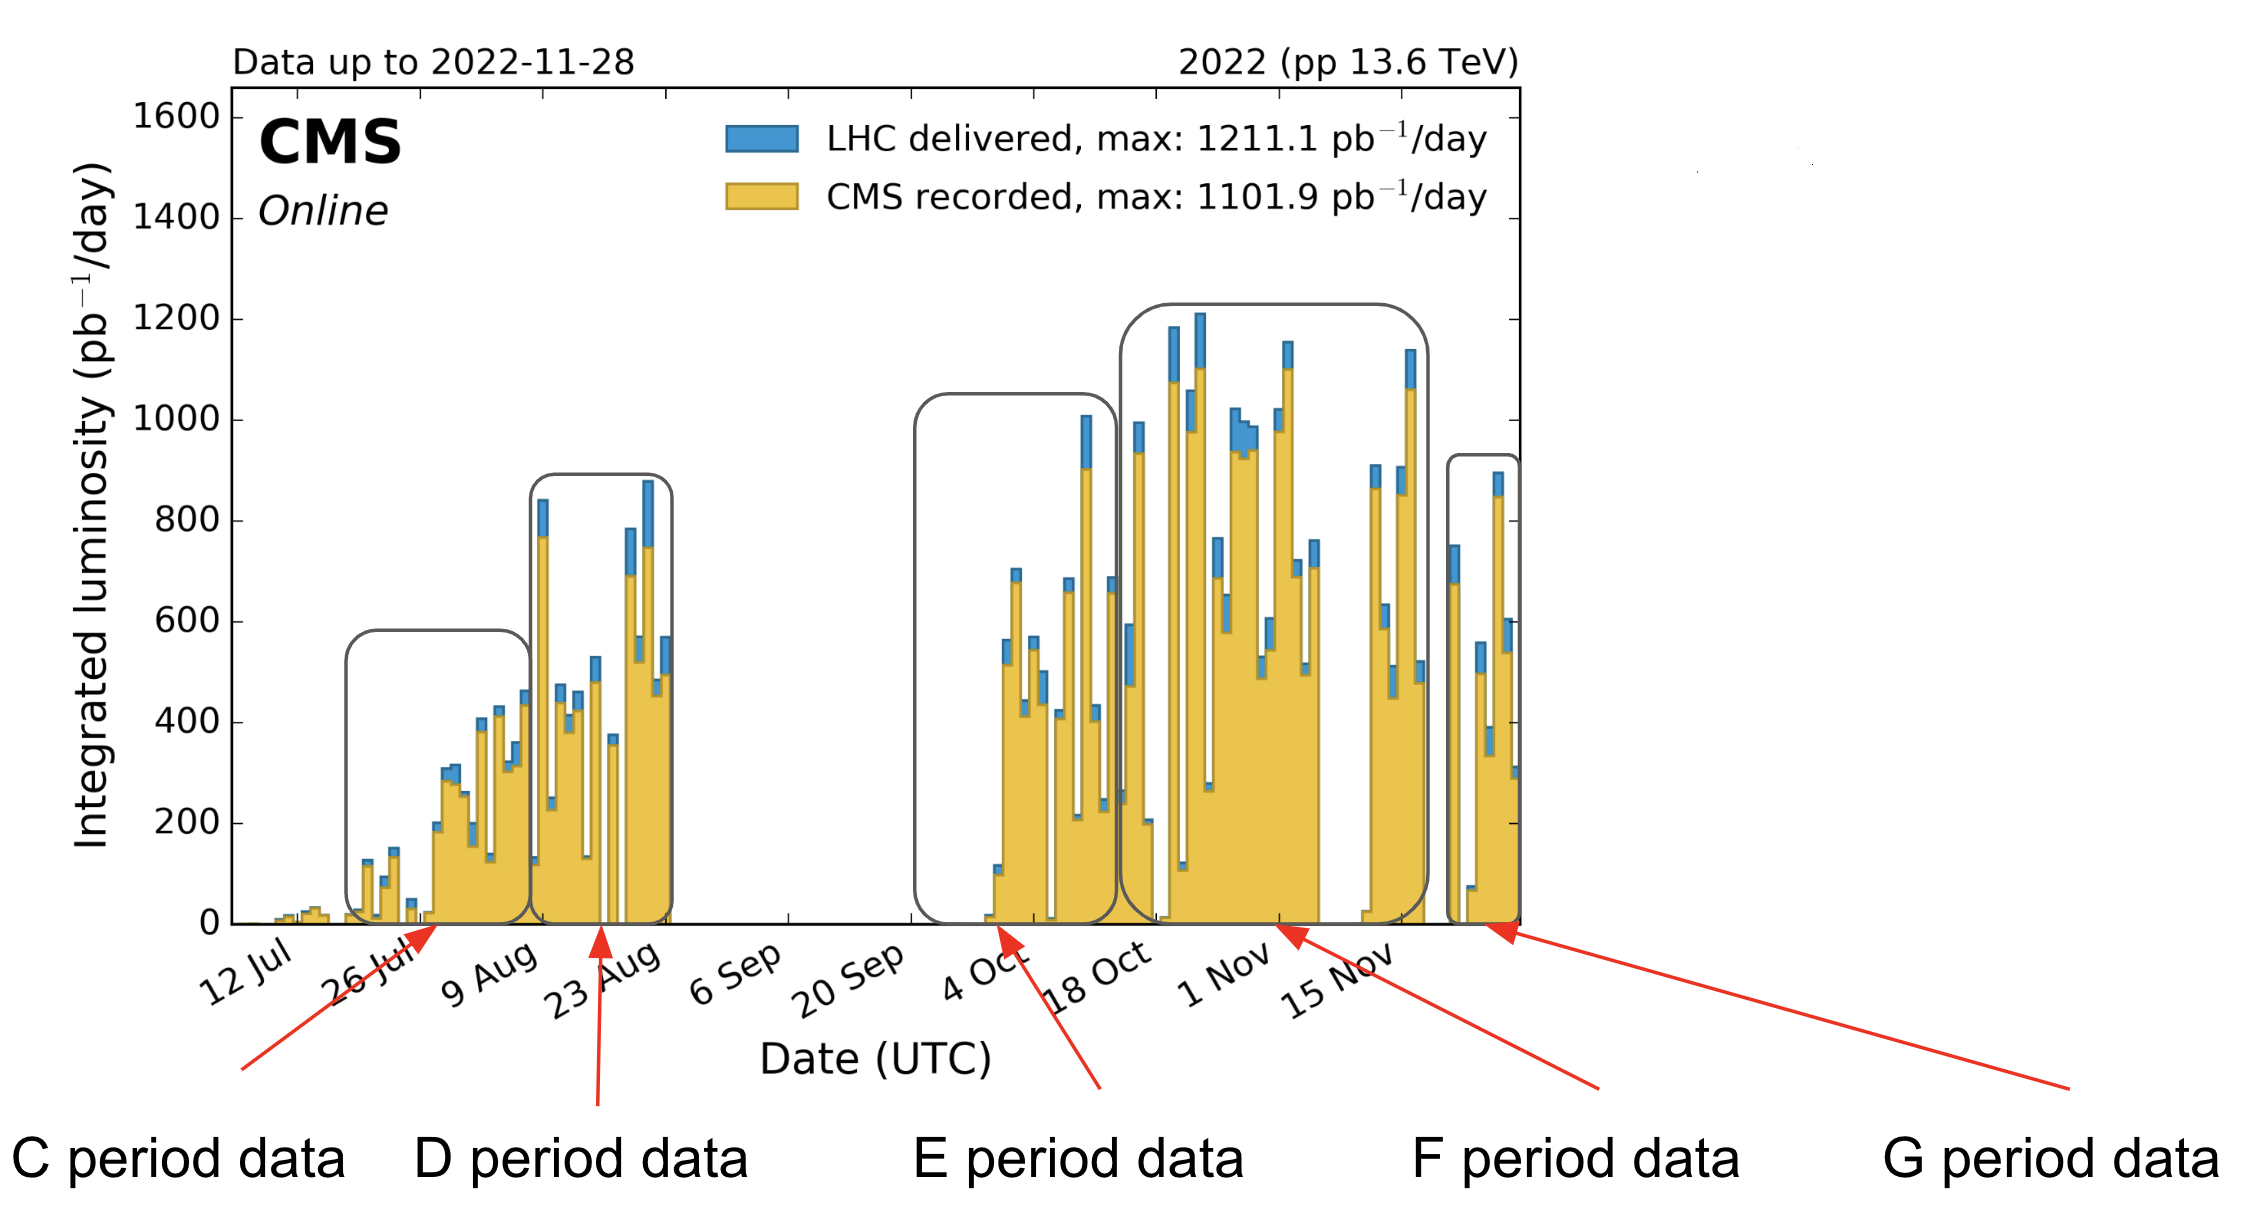
\includegraphics[width=1\textwidth]{ashish_thesis/2022_lumi_datasets.png}
\caption[2022 CMS luminosity data periods]{%                                                                                                                                              
   2022 luminosity data taking periods showing data taking period boundaries.
}
\label{fig:period_bound_1}
\end{figure}


\begin{table}[h]
  \centering
  \caption[2022 run ranges]{Run periods, run number ranges and dates for the 2022 data taking period.}
\begin{tabular}{ccc}
%\hline
\textbf{Run Period} & \textbf{Run Number Range} & \textbf{Date} \\
\hline
C & 355862 - 357401 & 2022-07-19 to 2022-08-12 \\
%\hline
D & 357538 - 357900 & 2022-08-15 to 2022-08-23 \\
%\hline
E & 359268 - 360327 & 2022-09-23 to 2022-10-14 \\
%\hline
F & 360390 - 362167 & 2022-10-14 to 2022-11-17 \\
%\hline
G & 362433 - 362760 & 2022-11-21 to 2022-11-28 \\
%\hline
\end{tabular}
%\caption[Run period details]{Run periods, run number ranges and dates.}
\label{tab:my_label_1}
\end{table}

\section{Detector module selection}

%The primary goal of PCC is to measure luminosity by counting charged particle clusters detected in the pixel detector, comprised of 1856 pixel modules. However, some modules are inconsistent due to issues like radiation damage or electronic malfunctions. To ensure accurate luminosity measurement, the performance of each module is continually assessed using a metric called the 'module weight', which is the ratio of a module's PCC to the total PCC as shown in Fig. \ref{fig:test}. If this weight shows significant fluctuations over time, the module might be unreliable. During each 23.36-second interval, termed a lumi section, an extensive analysis of these module weights is conducted.

The method for selecting reliable modules based on their performance, using the module weight, is detailed in section 4.2. Its significance in identifying consistent modules are illustrated in Fig. \ref{fig:test}. Evaluations are undertaken in lumi sections. Modules with consistent performance throughout 2022 are focused upon. Unreliable modules are added to a "module veto list", ensuring their data is excluded from luminosity calculation, thus preserving data accuracy. While all modules can be part of the luminosity measurement, only around 10\% withstand the rigorous selection criteria. The selection focuses on evaluating each module's stability using zero-bias dataset.

\begin{figure}[ht]
  \centering
  %\caption[Good and bad module weight profile]{Module weight profile showing good and bad module during Run 2022F.}
\begin{subfigure}{0.49\textwidth}
  \centering
  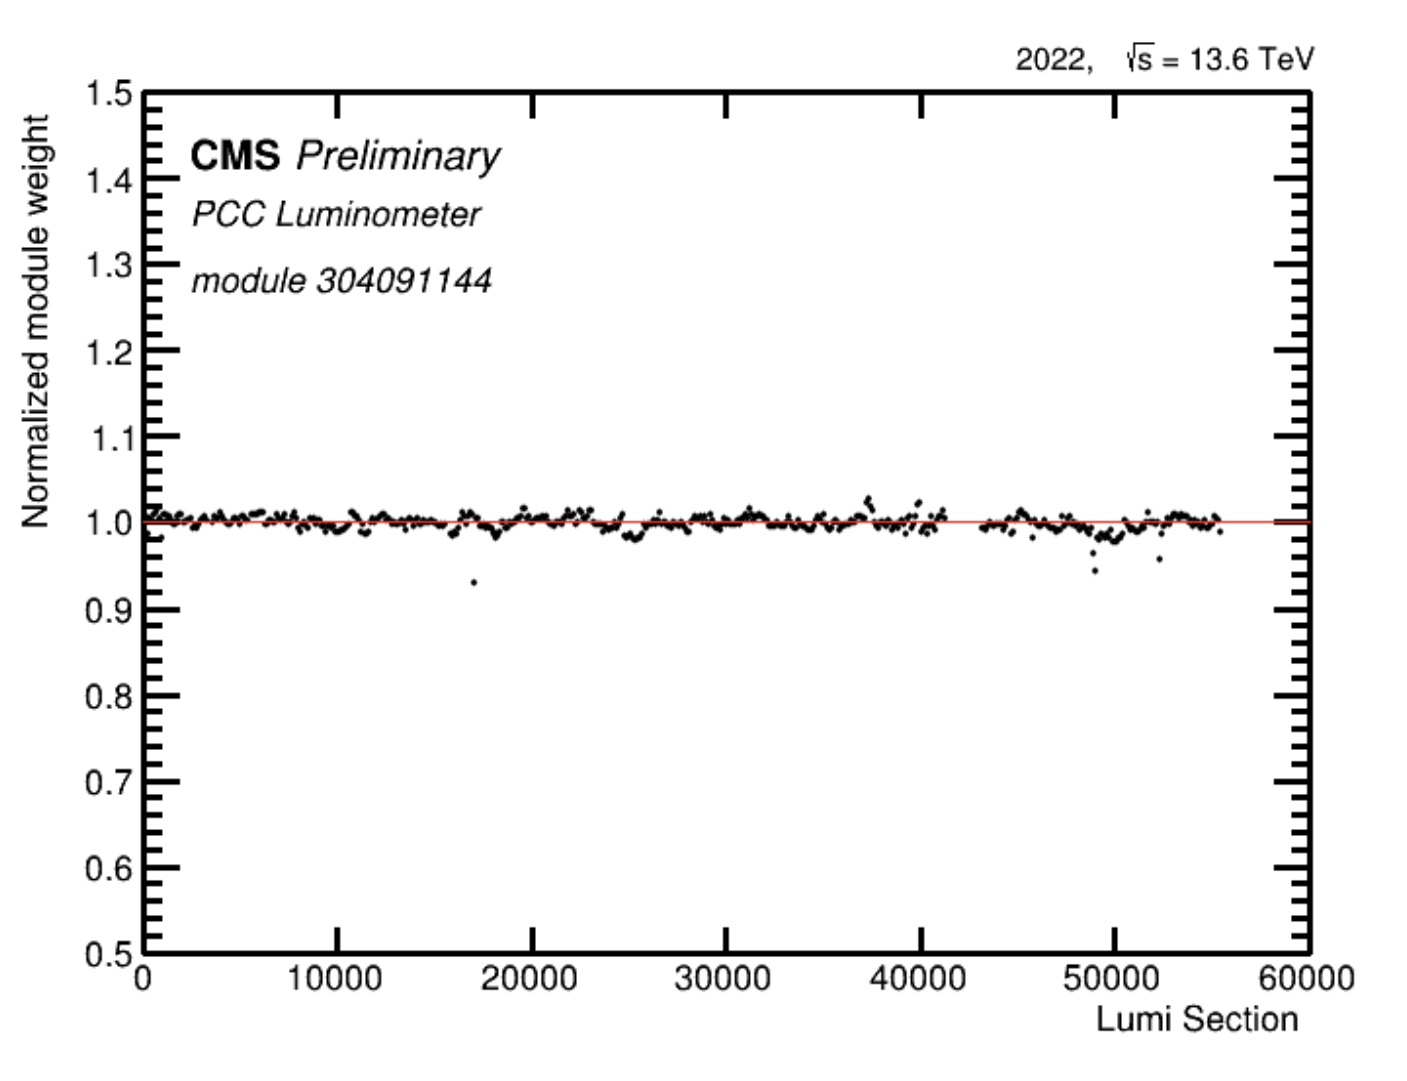
\includegraphics[width=1\linewidth]{ashish_thesis/2022_good_module_1.png}
  %\caption{}                                                                                                                                                                 
  \label{fig:sub1}
\end{subfigure}%                                                                                                                                                              
\begin{subfigure}{0.49\textwidth}
  \centering
  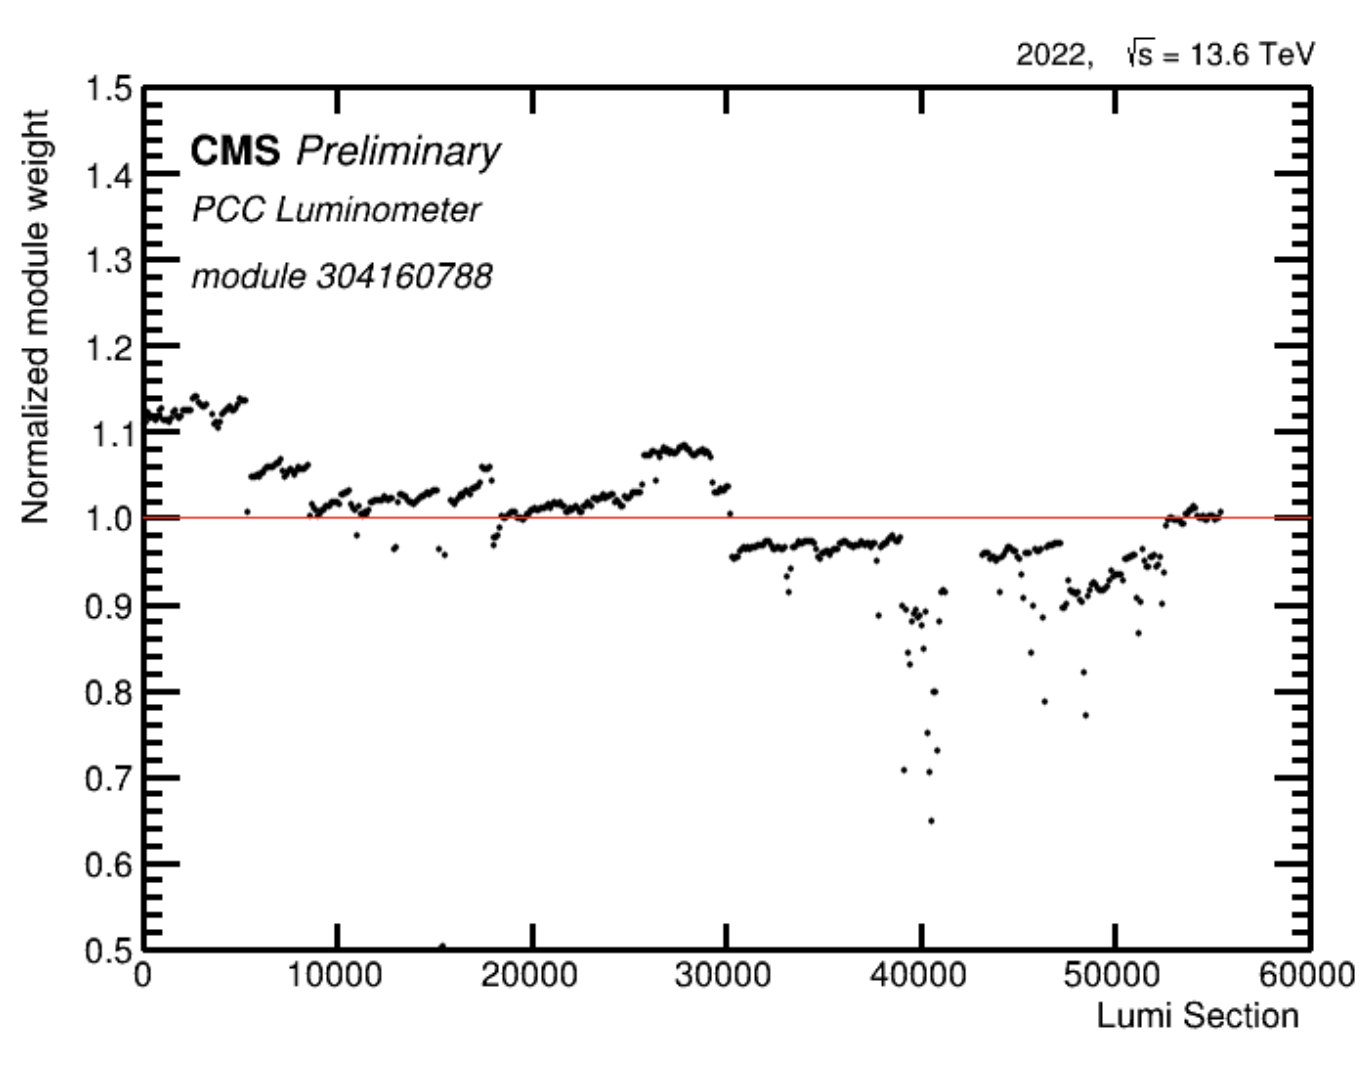
\includegraphics[width=1\linewidth]{ashish_thesis/2022_bad_module_1.png}
  %\caption{}                                                                                                                                                                 
  \label{fig:sub2}
\end{subfigure}
\caption[Good/Bad module weight profile]{Module weight profile as a function of lumi section showing good (left) and bad (right) module during Run 2022F. The horizontal red line is the mean of the module weight.}
\label{fig:test}
\end{figure}

%\begin{itemize}
 %   \item \textbf{Stability over Time:} Modules maintaining consistent relative contributions during standard physics runs are retained. If they deviate beyond an initial 5-10\% range, as gauged by the RMS-to-Mean distribution of cluster counts, they're excluded. This exclusion process is repeated two or three times, removing outliers with each iteration as shown in Fig. \ref{fig:stab_deviation_2022}.

  %  \item \textbf{Linearity:} The analysis centers on a module's response to instantaneous luminosity, measured by the average Pixel Cluster Count (PCC) per module. Two figures elucidate this: one detailing an individual module's response and another offering a cumulative histogram for all modules as shown in Fig. \ref{fig:lin_deviation_2022}.
%\end{itemize}

For module evaluation, the steps include:
\begin{enumerate}
    \item Lumi sections with low statistics are removed based on total PCC.
    \item All barrel Layer-0 modules are sidestepped due to their vulnerability to dynamic inefficiency.
    \item An intial filtering removes modules with 2\% average deviation of the module weight from its mean (shown in Fig. \ref{fig:stab_deviation_2022}). %Subsequent adjustments tighten this criterion, illustrated by further refinements to 2\% and 0.8\% respectively.

    \item Module stability is reviewed using an iterative method. In the case of the 2022F dataset, we introduce additional criteria of 0.8\%. For different data periods, the specific values used depend on how good the initial module list is.

    \item The selection of modules based on their linearity relies on assessing the average deviation of the module weight v.s. the average PCC per module (shown in Fig. \ref{fig:lin_deviation_2022}). This process typically requires either one or two iterations. To illustrate, during the 2022F period, we first apply a 0.4\% selection criterion, followed by a more stringent 0.25\% selection.

\end{enumerate}

%The quality of the initial module list determines the precision in ensuing data periods. For periods C, D, E, and G, the Run 2022F module veto list is used as a starting point. During the vdM fill, modules evincing instability or high noise are dismissed. %Table \ref{tab:bad_modules} delivers a comprehensive rundown of omitted modules for the 2022 datasets.

\begin{figure}[!htp]
  \centering
  %\caption[2018 CMS luminosity data taking periods]{ 2022 luminosity data taking periods showing data taking period boundaries.}                                                                                              
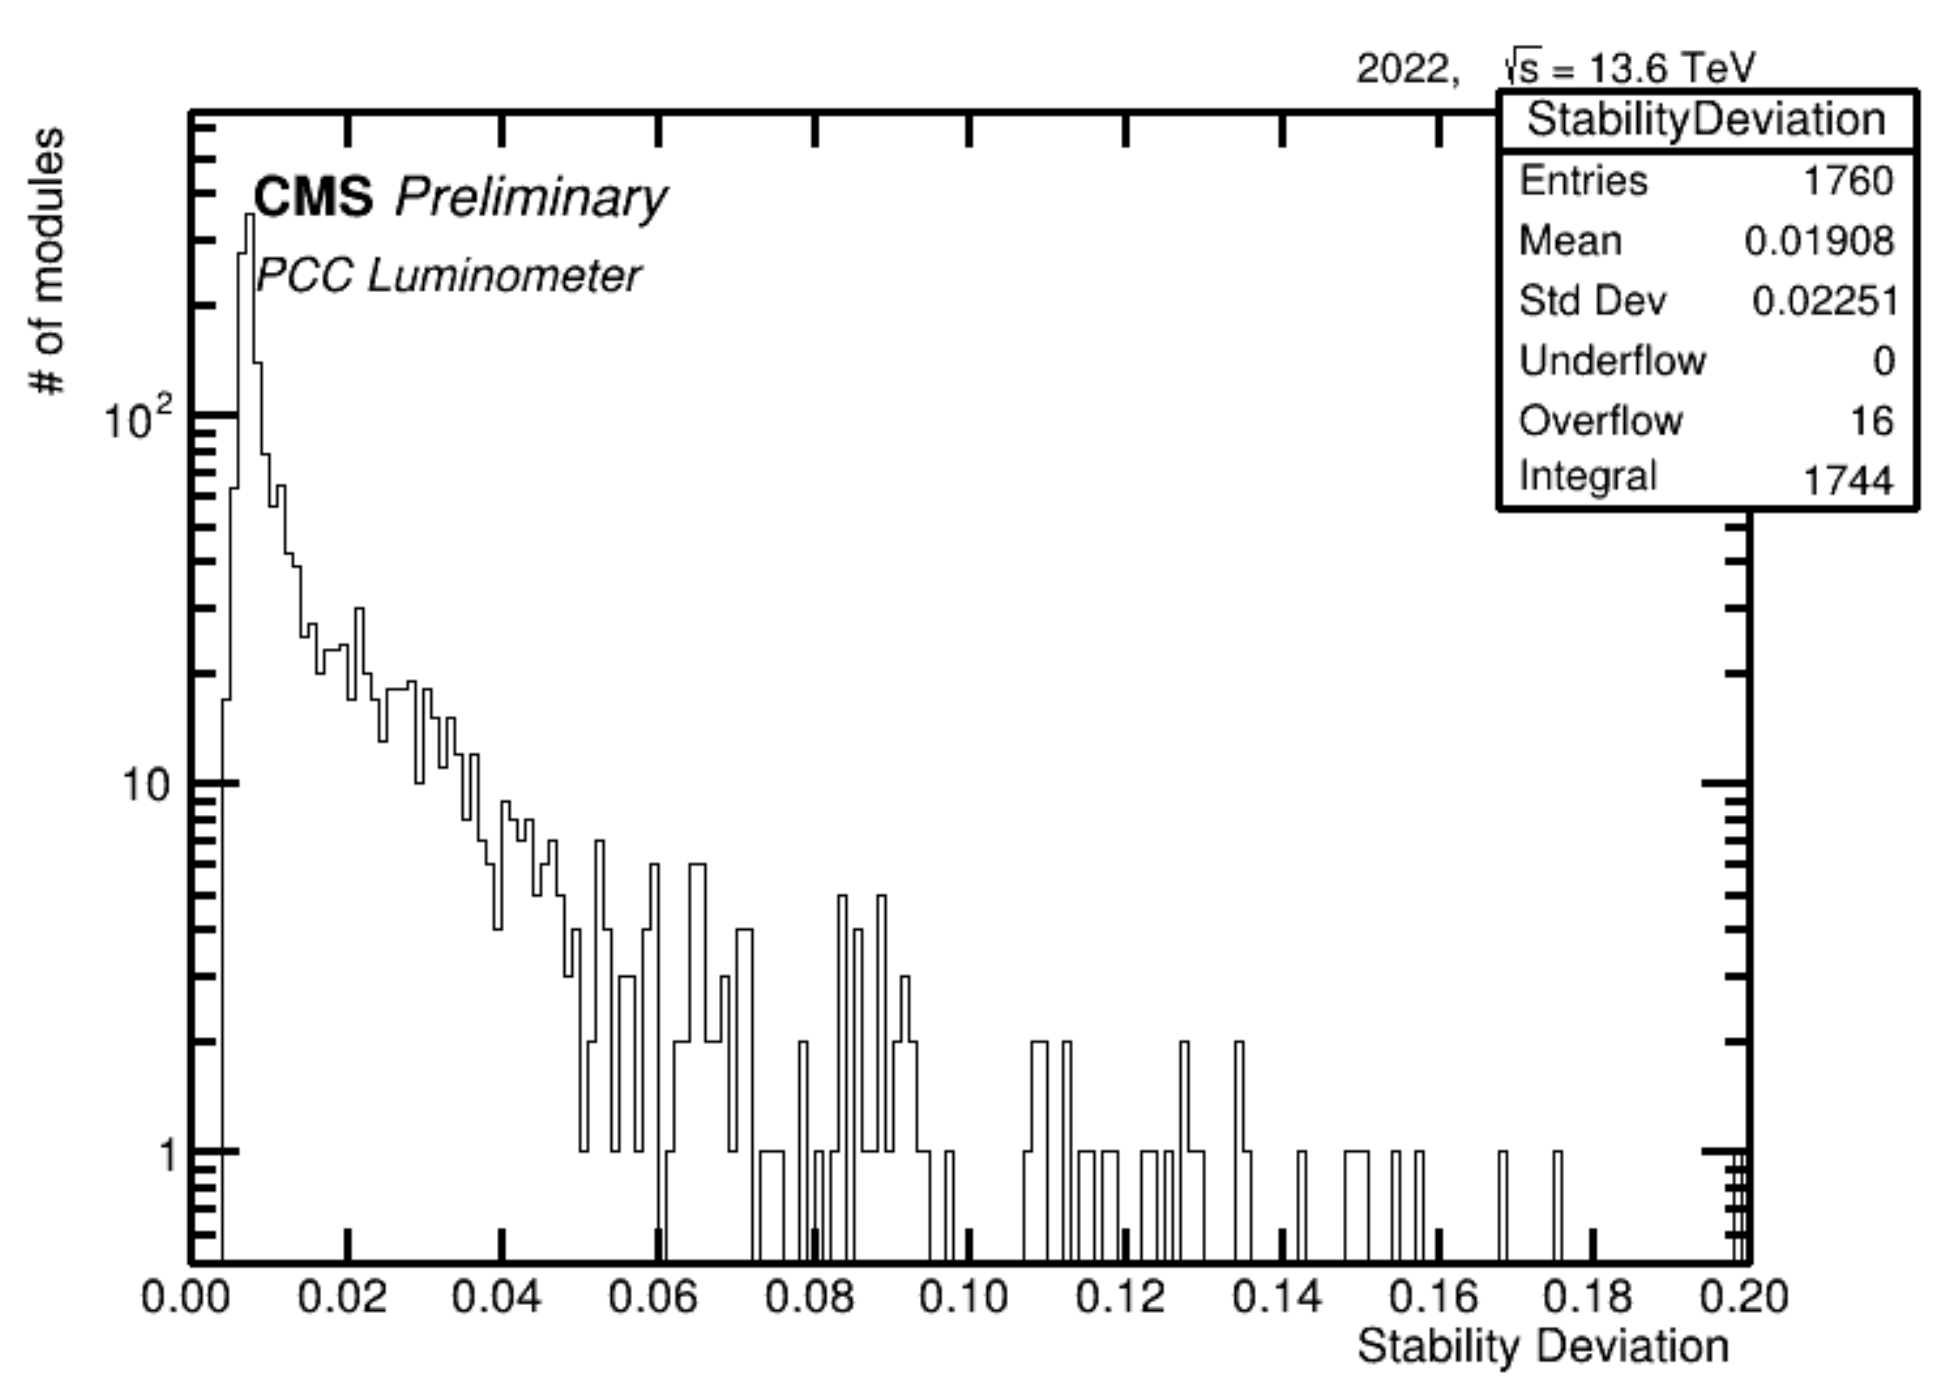
\includegraphics[width=1\textwidth]{ashish_thesis/stability_deviation_2022_1.png}
\caption[Module weight standard deviation]{%
  During Run 2022F, the distribution illustrates the average deviation of the module weight over it's mean for all modules.
}
\label{fig:stab_deviation_2022}
\end{figure}

\begin{figure}[!htp]
  \centering
  %\caption[2018 CMS luminosity data taking periods]{ 2022 luminosity data taking periods showing data taking period boundaries.}                                                                                              
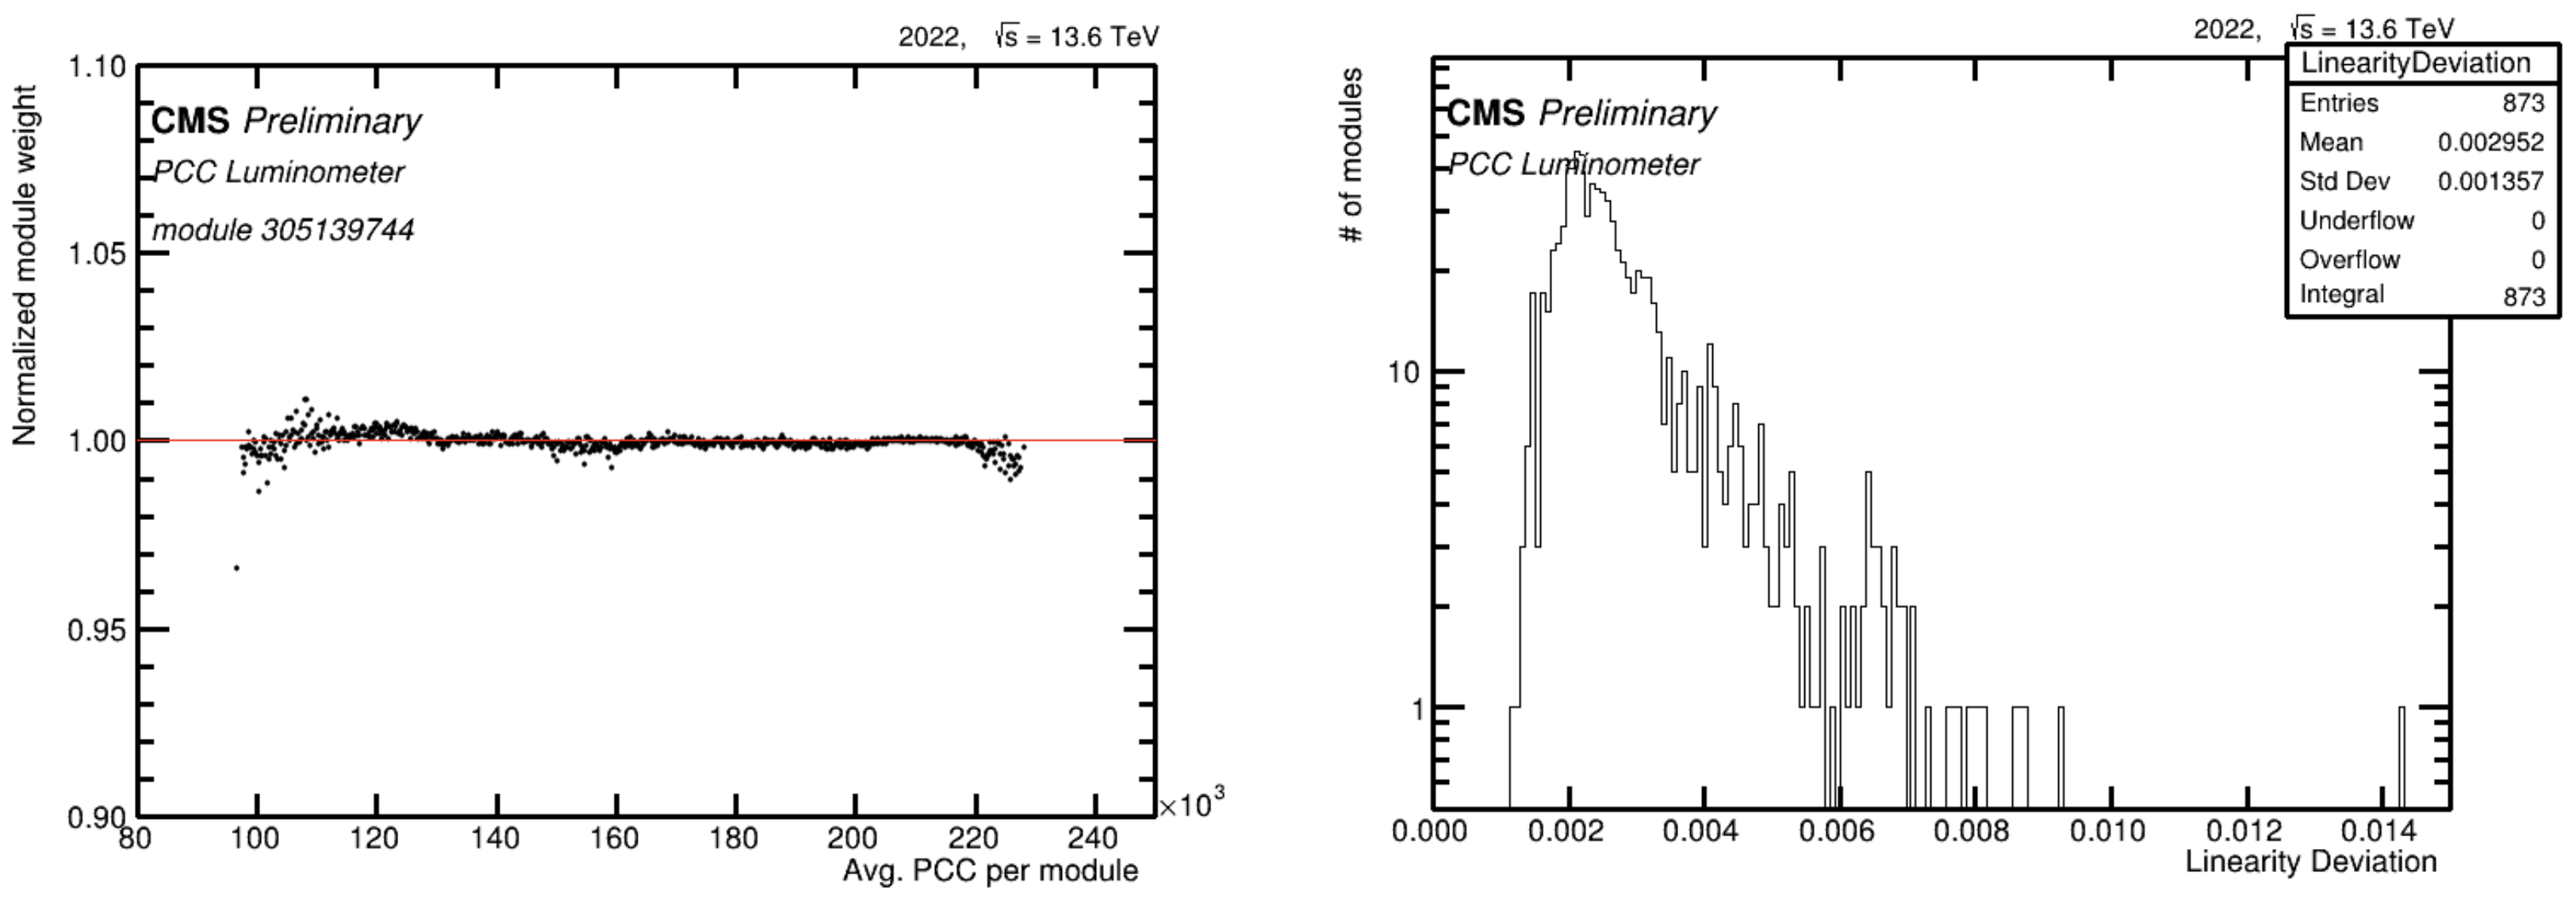
\includegraphics[width=1\textwidth]{ashish_thesis/linearity_deviation_2022_1.png}
\caption[Module linearity & linearity deviation distribution]{%
 Left: Linearity profile, module weight as a function of average PCC per module for one module in Run 2022F. Right: For all modules in Run 2022F, the distribution displays average deviations of the module weight divided by their mean derived from their linearity profiles.
}
\label{fig:lin_deviation_2022}
\end{figure}

%The objective of reducing fluctuations in the PCC luminosity measurement is to guarantee accurate and reliable results. This is accomplished by creating a pixel module veto list for each time period to monitor and exclude problematic modules. The stability of each module is assessed by tracking the fluctuation in the ratio of the module's PCC to the total PCC, a value termed as the module weight, as demonstrated in Fig. \ref{fig:test}. The data acquired for luminosity measurements is partitioned into sections referred to as lumi sections, each spanning a duration of 23.36 seconds. During each lumi section, an in-depth analysis of the module weights for all pixel modules is carried out to monitor their performance progression over time. This critical step aids in the distinction between efficient and inefficient modules. The pixel modules selected for consideration are those that demonstrate a consistently reliable performance throughout the entirety of 2022. %Any modules failing to meet these standards are deemed inefficient and are hence excluded from the luminosity measurement. Through meticulous examination of the module weights and the strategic exclusion of inefficient modules from the study, we can substantially reduce instabilities in PCC luminosity measurement. This rigorous process assures the high quality of data used for luminosity measurement, paving the way for precision in the obtained results.

\begin{comment}
  
\begin{figure}[ht]
\centering
\begin{subfigure}{0.49\textwidth}
  \centering
  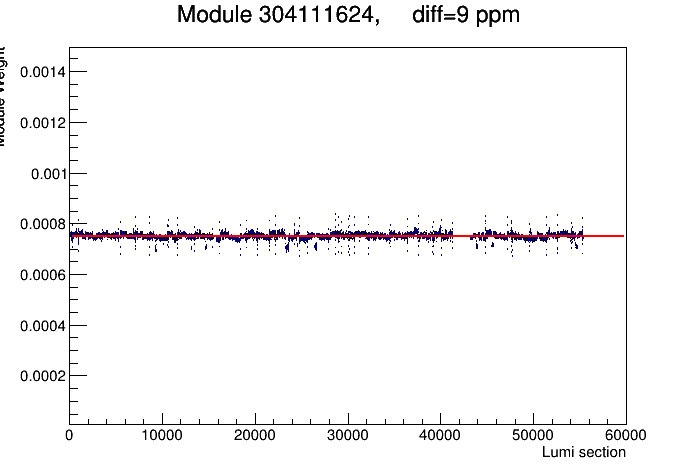
\includegraphics[width=1\linewidth]{ashish_thesis/2022_good_module.png}
  %\caption{}
  \label{fig:sub1}
\end{subfigure}%
\begin{subfigure}{0.49\textwidth}
  \centering
  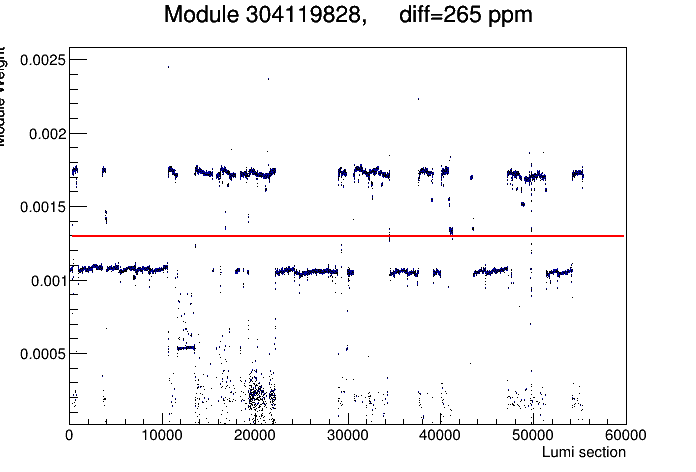
\includegraphics[width=1\linewidth]{ashish_thesis/2022_bad_module.png}
  %\caption{}
  \label{fig:sub2}
\end{subfigure}
\caption[Good and bad module weight profile]{Module weight profile showing good and bad module during Run 2022F.}
\label{fig:test}
\end{figure}

\end{comment}

%The basic premise of PCC is to count the number of clusters of charged particles detected in the pixel detector, and use this count to calculate the luminosity. The pixel detector is composed of thousands of small, sensitive components known as pixel modules. These pixel modules detect and measure particles passing through them, which provides the raw data used to calculate luminosity. However, not all pixel modules perform consistently. Factors like radiation damage, aging, or electronic faults can cause a module to give incorrect or inconsistent readings. When a module isn't working correctly, its data can introduce significant errors into the luminosity measurement. If a module is found to be performing poorly or inconsistently, it is added to a "module veto list." This list is a record of all the pixel modules that have been identified as unreliable. The 'veto' in the module veto list refers to the act of explicitly excluding or disregarding the data from the listed modules in the luminosity calculation to prevent them from skewing the results. %Creating and maintaining the module veto list is a complex process that requires continual monitoring and analysis.
%For each data-taking period, the module weight, which is the ratio of a module's PCC to the total PCC, is computed and tracked. If the module weight shows significant or unexplained variations, that could be a sign that the module is not performing correctly, and it may be added to the veto list. By doing so, the impact of these 'bad' modules is eliminated, and the luminosity measurement is improved, leading to more reliable and accurate data. %In essence, the module veto list is an important quality control tool used in the CMS experiment to ensure the highest possible accuracy and precision in their luminosity measurement.

%Figure \ref{fig:period_bound_3} describes the distribution of the ratio of Root Mean Square (RMS) to the mean of the module weight profile for all modules. The module weight is a representation of each module's performance. The RMS over the mean provides a measure of the variation in the module weights. In this figure, a preliminary selection criterion of 7\% is used to identify and exclude 'bad' or poorly performing modules, i.e., modules whose RMS to mean ratio exceeds 7\% are considered bad and removed.

%This process is iterative, employing different selection thresholds at each stage to systematically identify and exclude bad modules. Figure \ref{fig:period_bound_4} illustrates the RMS over mean module weight distribution, after second iterative selection step have been completed. Here, a stricter selection criterion of 4\% is applied. This means that any modules with an RMS to mean ratio exceeding 4\%, even after all previous selection stages, are added to the veto list for each period. These modules' data are excluded from the luminosity measurements for their respective period. Table \ref{tab:bad_modules} delivers a comprehensive rundown of omitted modules for the 2022 dataset.  %The entire process, as depicted in these figures, is intended to ensure that the PCC luminosity measurement rely solely on data from the most stable and reliable modules, thereby enhancing the accuracy and precision of these measurement.

Table \ref{tab:bad_modules} presents a quantitative summary of malfunctioning or "bad" modules across various periods. BPIX Layer0 has 96 bad modules. As we progress through the various periods in 2022 (from F to D), there is a general trend of increasing bad modules, both for stability and linearity considerations. The total number of bad modules  added to the veto list grows in each period due to the sequential or iterative nature of the procedure where the veto list for each period starts with the veto from the previous period \cite{pas_22}.


This suggests that as time progresses, the number of malfunctioning modules tends to grow. The highest number of bad modules for stability is observed in the 2022D period with 1653 bad modules. On the other hand, the 2022D period also has the highest for linearity with 1677 bad modules. The vdM fill has 1693 bad modules, which is slightly higher than those in the 2022D period for stability but slightly less for linearity. There seems to be a consistent observation that for each given period, the number of bad modules under linearity considerations is either equal to or slightly higher than those under stability considerations \cite{pas_22}. % \cite{bril2023moduleveto}.

\begin{table}[h]
  \centering
  \caption[Bad modules per period]{Number of bad modules for selection on stability and linearity for various periods.}
\begin{tabular}{lr}
\textbf{Type Or Period/Step} & \textbf{\# of bad modules} \\
\hline
BPIX Layer0 & 96 \\
2022F Stability & 983 \\
2022F Linearity & 1195 \\
2022C Stability & 1364 \\
2022C Linearity & 1484 \\
2022E Stability & 1553 \\
2022E Linearity & 1570 \\
2022G Stability & 1604 \\
2022G Linearity & 1628 \\
2022D Stability & 1653 \\
2022D Linearity & 1677 \\
vdM fill & 1693 \\
\end{tabular}
%\caption{Number of bad modules for selection on stability and linearity for various periods.}                                                                                                            
\label{tab:bad_modules}
\end{table}


\begin{table}
\centering
\caption{Number of good modules in each layer/disk}
\label{tab:2022ldmodules}
\begin{tabular}{cc}
\textbf{Layer/Disk} & \textbf{Number of Good Modules} \\
\hline
Layer 3 & 39 \\
Layer 4 & 88 \\
Disk 1 & 13 \\
Disk 2 &  19\\
Disk 3 &  4\\
Total & 163\\
% Add more empty rows as needed
\end{tabular}
\end{table}

Table \ref{tab:2022ldmodules} presents the number of good modules in various layers and disks of the pixel detector after a final selection process. %Layer 3 has 39 good modules, Layer 4 has 88, Disk 1 has 13, Disk 2 has 19, and Disk 3 has 4, totaling 163 modules.
The stability of various pixel layers and disks after removing all modules in Layer 0 and for final veto are shown in Fig. \ref{fig:stabprof_69a}  and Fig. \ref{fig:stabprof_69b} respectively.

\begin{comment}

\begin{figure}[!htp]
\centering
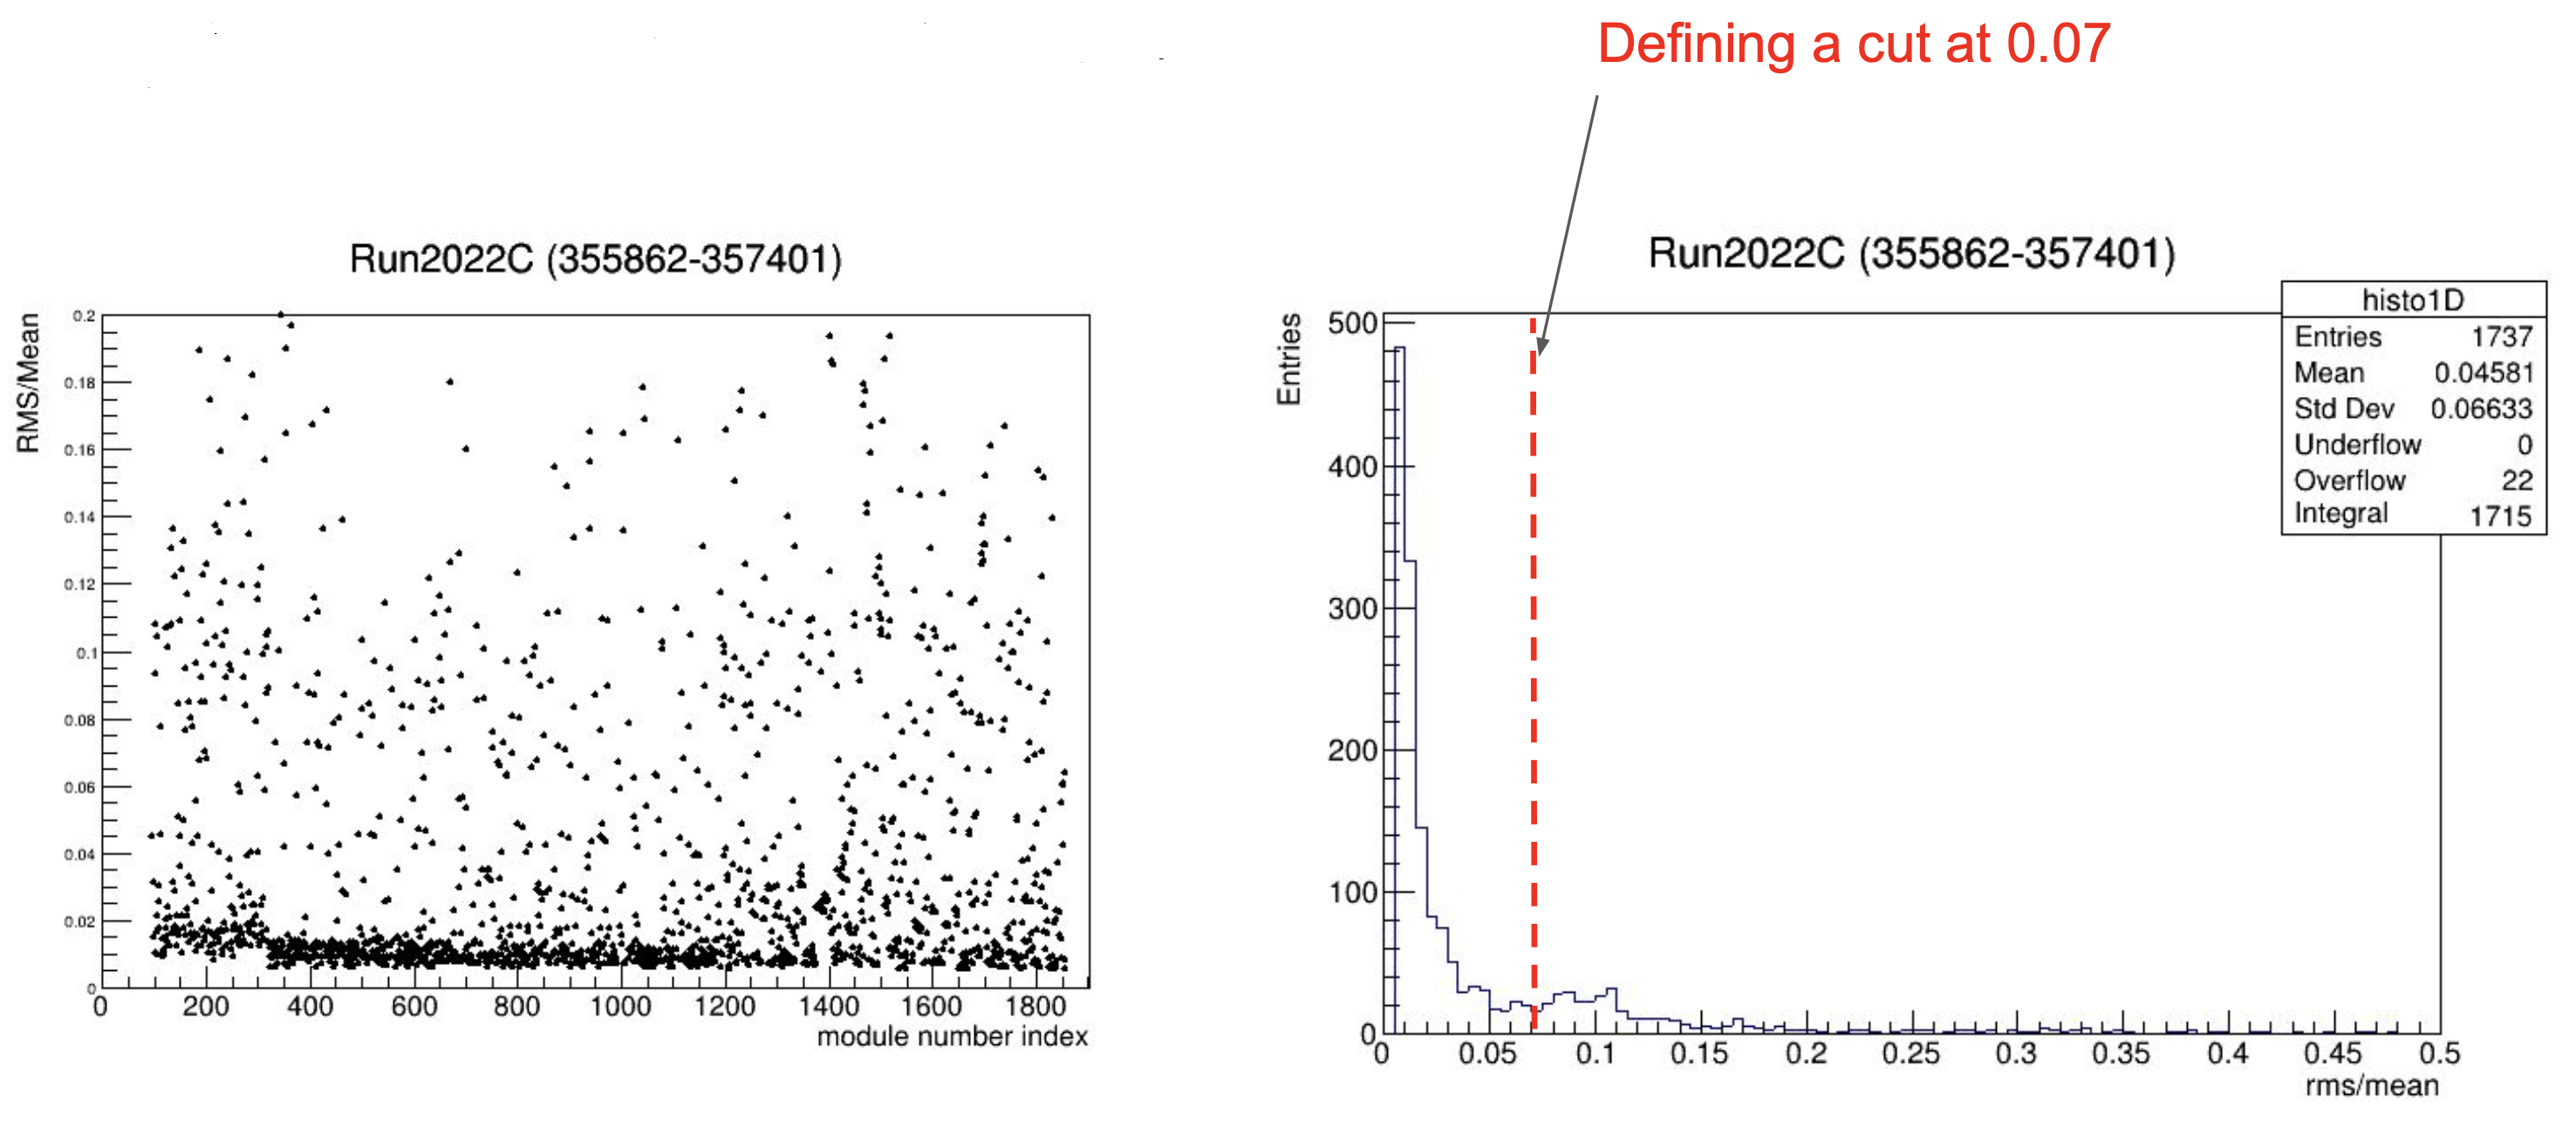
\includegraphics[width=1\textwidth]{ashish_thesis/2022_periodC_first_iteration}
\caption[First Iteration to Remove Outlier Modules]{%
  RMS/mean of module weight profile for all modules. A loose selection of 7\% is applied to remove bad modules. Appropriate selections are applied in each iterative step to remove other bad modules.
}
\label{fig:period_bound_3}
\end{figure}

\begin{figure}[!htp]
\centering
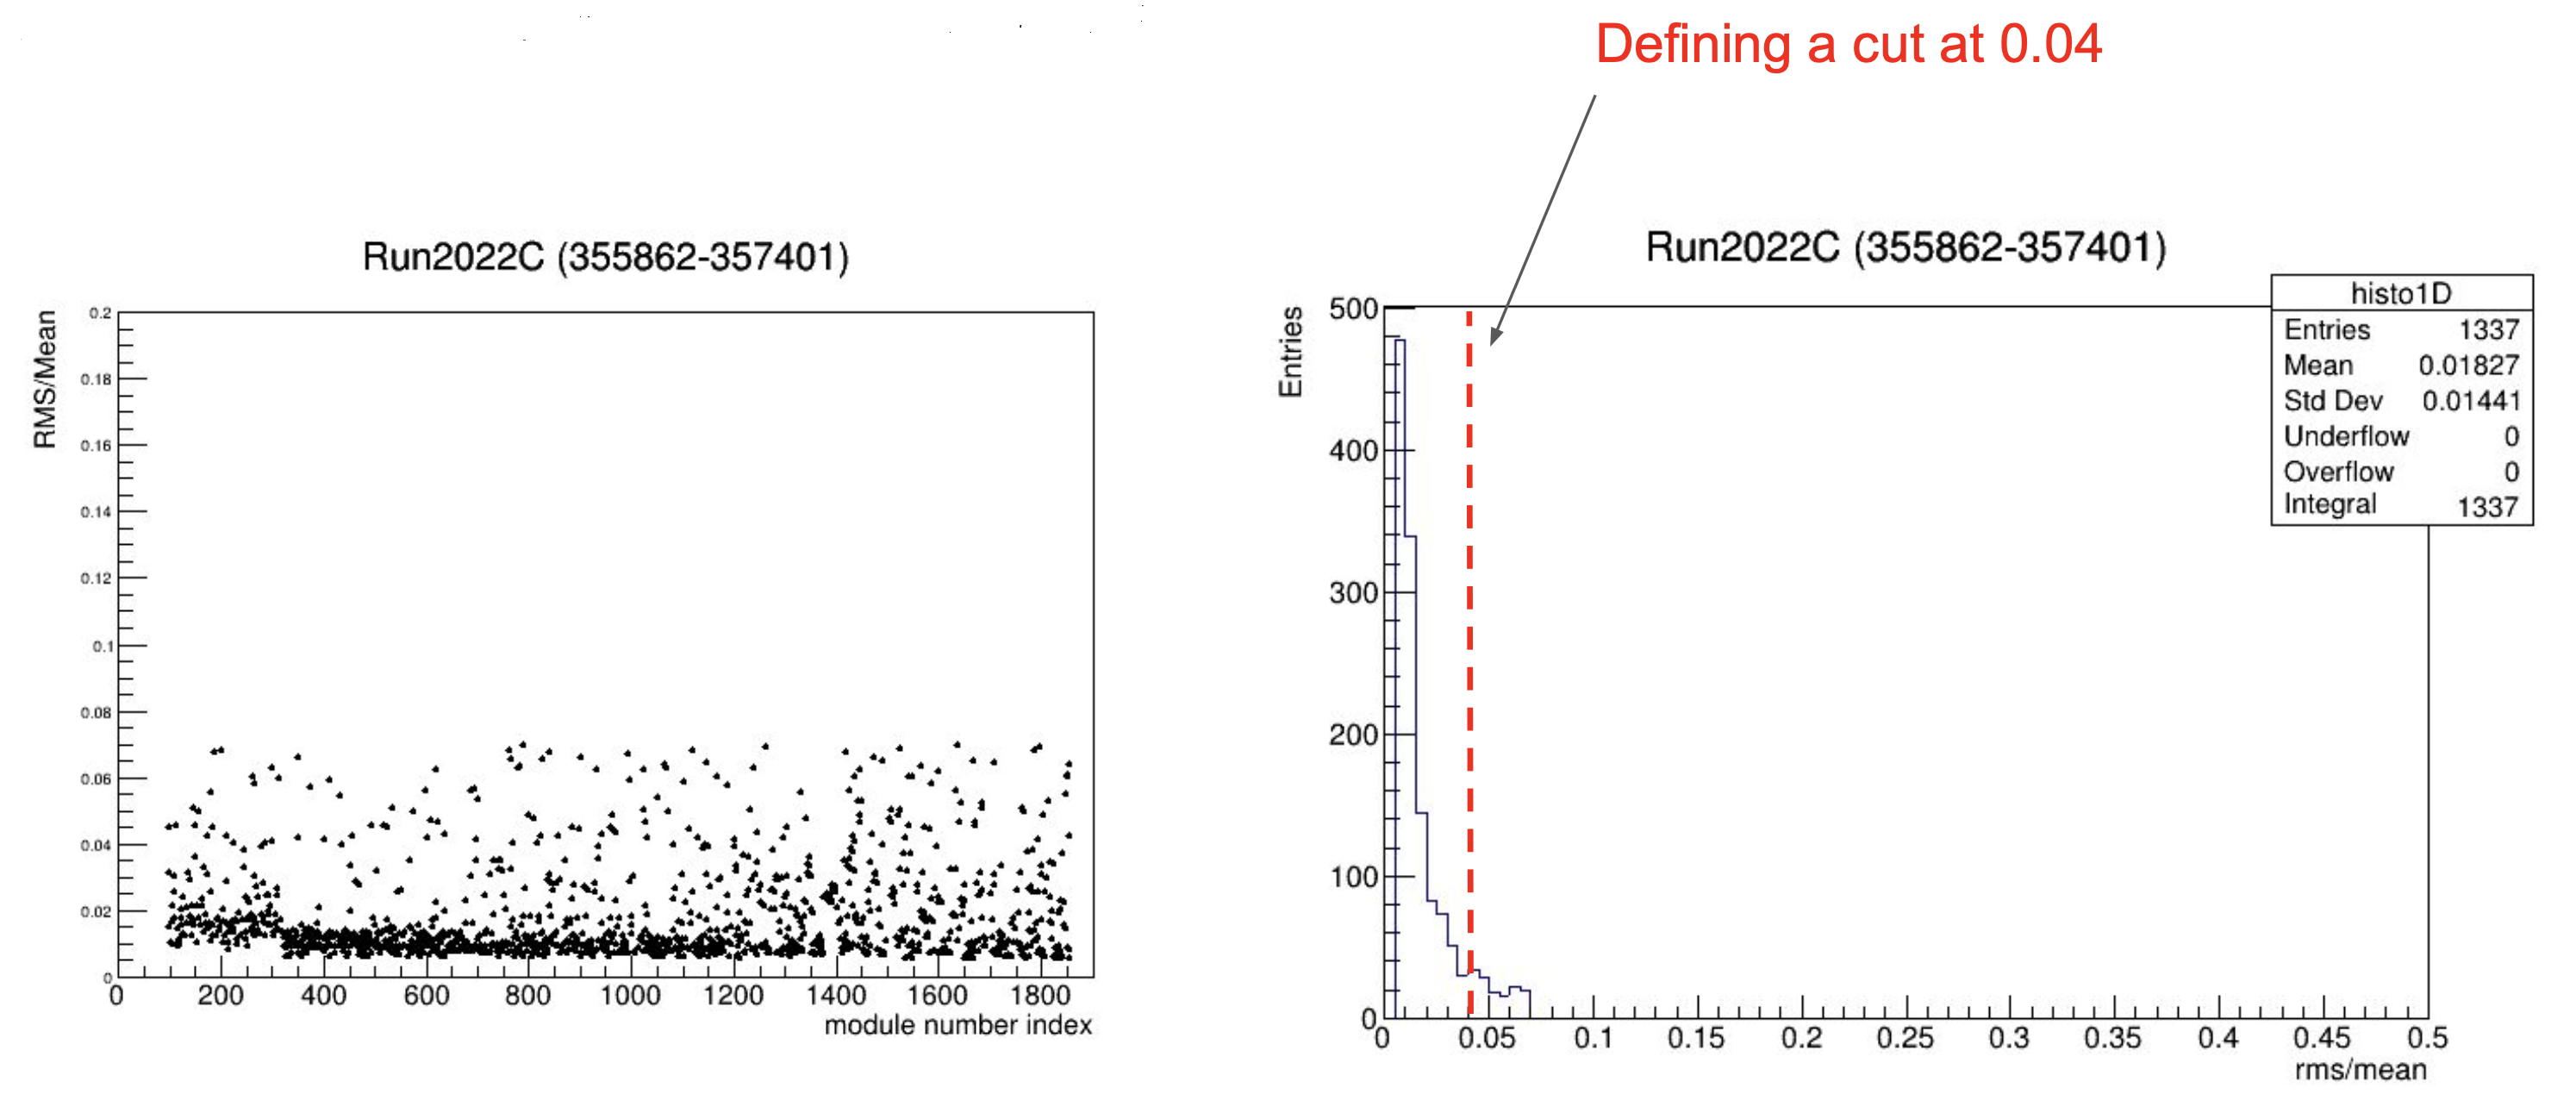
\includegraphics[width=1\textwidth]{ashish_thesis/2022_periodC_final_iteration.png}
\caption[Final Iteration To Remove Outlier Modules]{%
 Second selection on RMS/mean of 4\% is applied.}
}
\label{fig:period_bound_4}
\end{figure}

\end{comment}

%\begin{figure}[!htp]
%\centering
%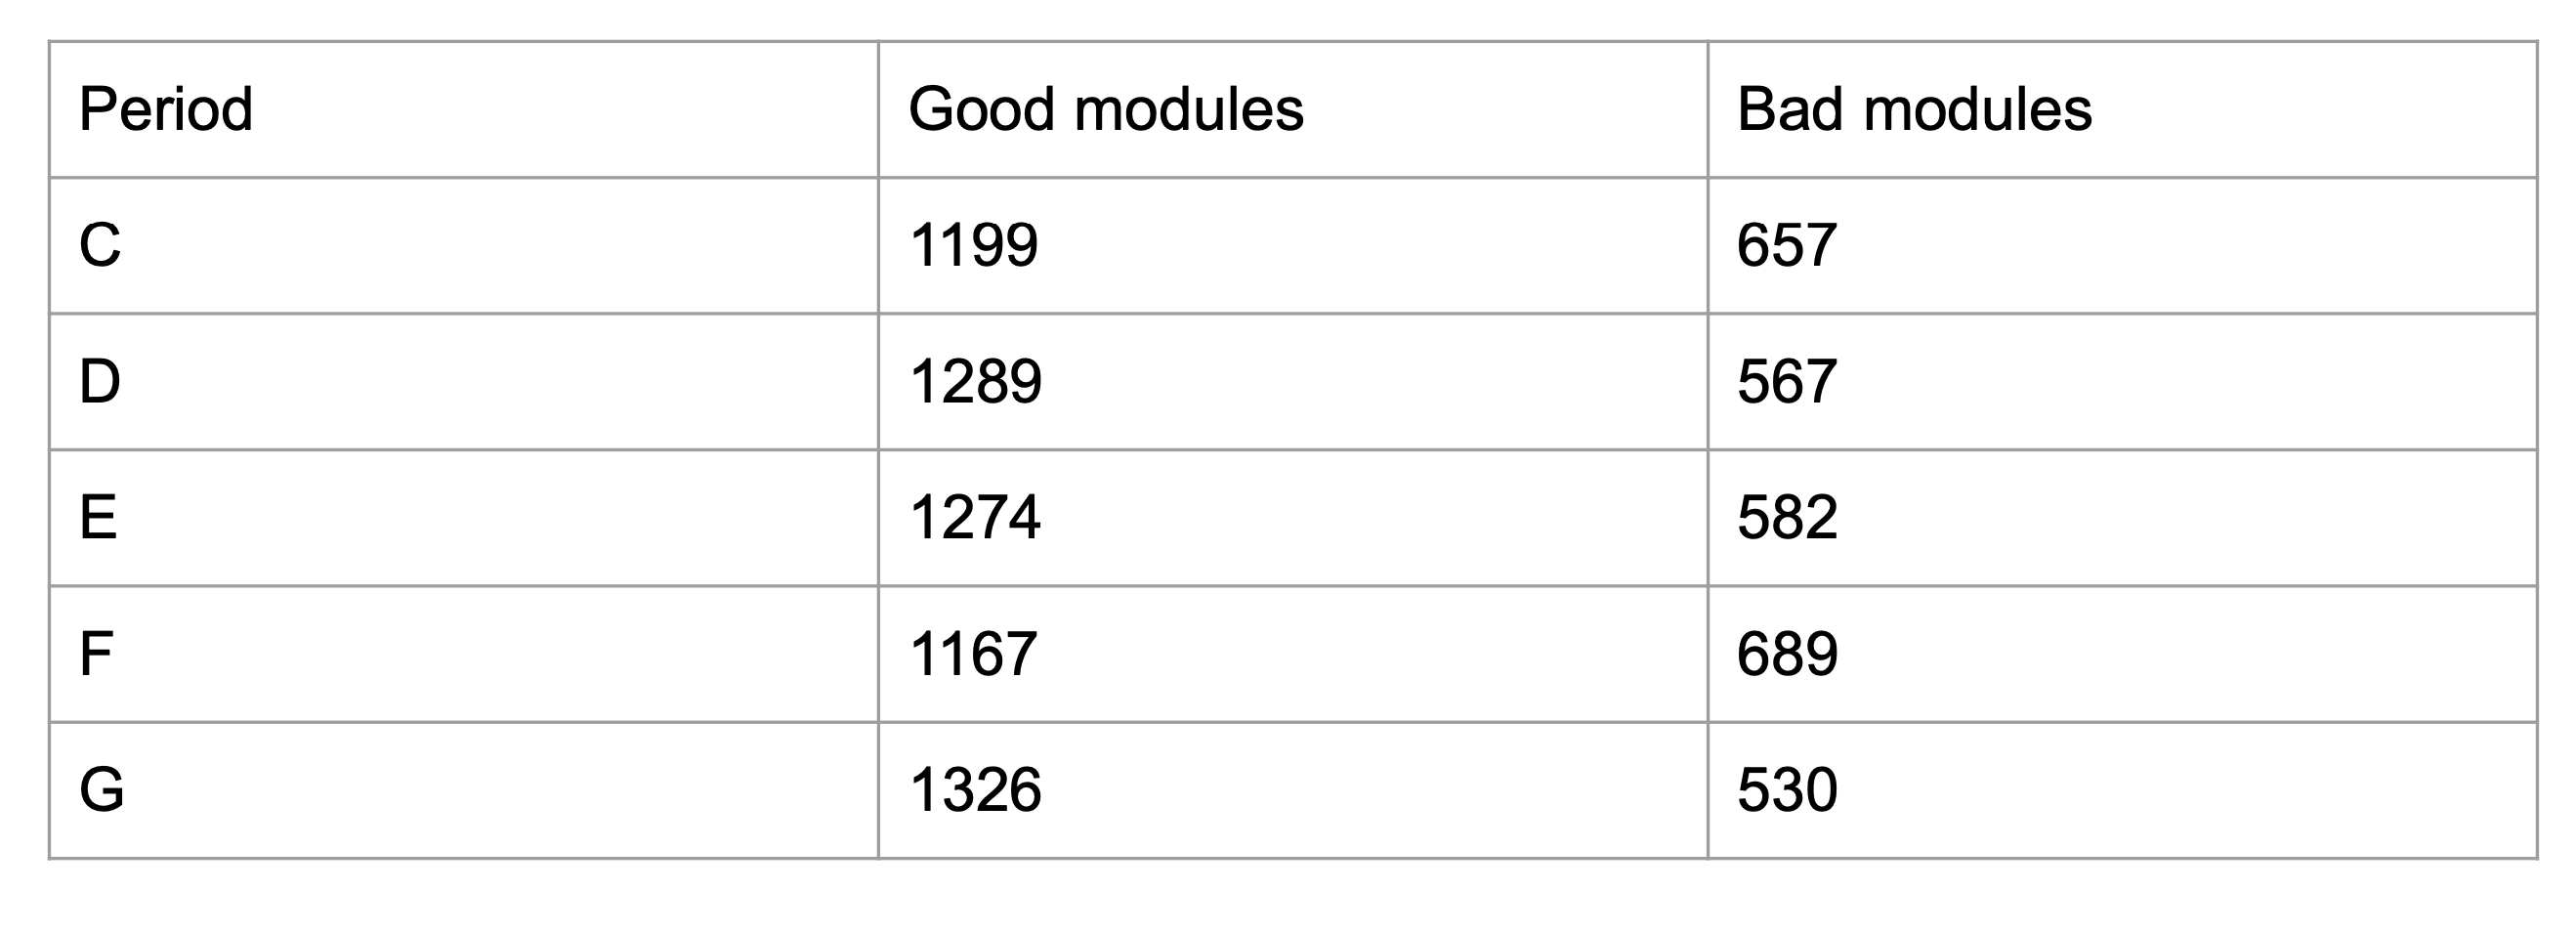
\includegraphics[width=1\textwidth]{ashish_thesis/2022_per_period_veto.png}
%\caption[2018 CMS luminosity data taking periods.]{%                                                                                                                                         
 % 2022 luminosity data taking periods showing data taking period boundaries and vdM calibration data .
%}
%\label{fig:period_bound}
%\end{figure}

\begin{comment}

Table \ref{table:1_2022} presents a summary of the number of good and bad pixel modules identified for different periods (C, D, E, F, and G) during the 2022 PCC luminosity measurement. It is structured into three columns: 'Period', 'Good Modules', and 'Bad Modules'. The 'Period' column lists the periods during which the luminosity measurements were taken. These are represented as C, D, E, F, and G. The 'Good Modules' column shows the count of pixel modules that consistently performed well and provided reliable data for each respective period. For instance, there are 1198 good modules in period C, 1289 in period D, and so on. The 'Bad Modules' column displays the number of pixel modules that were identified as problematic or unreliable during each period. These modules have shown signs of inconsistent performance, thereby added to the veto list. For example, there are 658 bad modules during period C, 567 in period D. It allows a clear comparison between the periods in terms of the quality of modules used in the luminosity measurements, highlighting the different counts of good and bad modules identified during each period.

\begin{table}[h!]
  \centering
  \caption[2022 period veto]{Good and bad modules for each period using per period veto.}
\begin{tabular}{ccc}
\textbf{Period} & \textbf{Good Modules} & \textbf{Bad Modules} \\
\hline
C & 1198 & 658 \\
D & 1289 & 567 \\
E & 1274 & 582 \\
F & 827 & 1029 \\
G & 1347 & 509 \\
\end{tabular}
%\caption[2022 per period veto]{Good and bad modules for each period using per period veto.}
\label{table:1_2022}
\end{table}

%\begin{figure}[!htp]
%\centering
%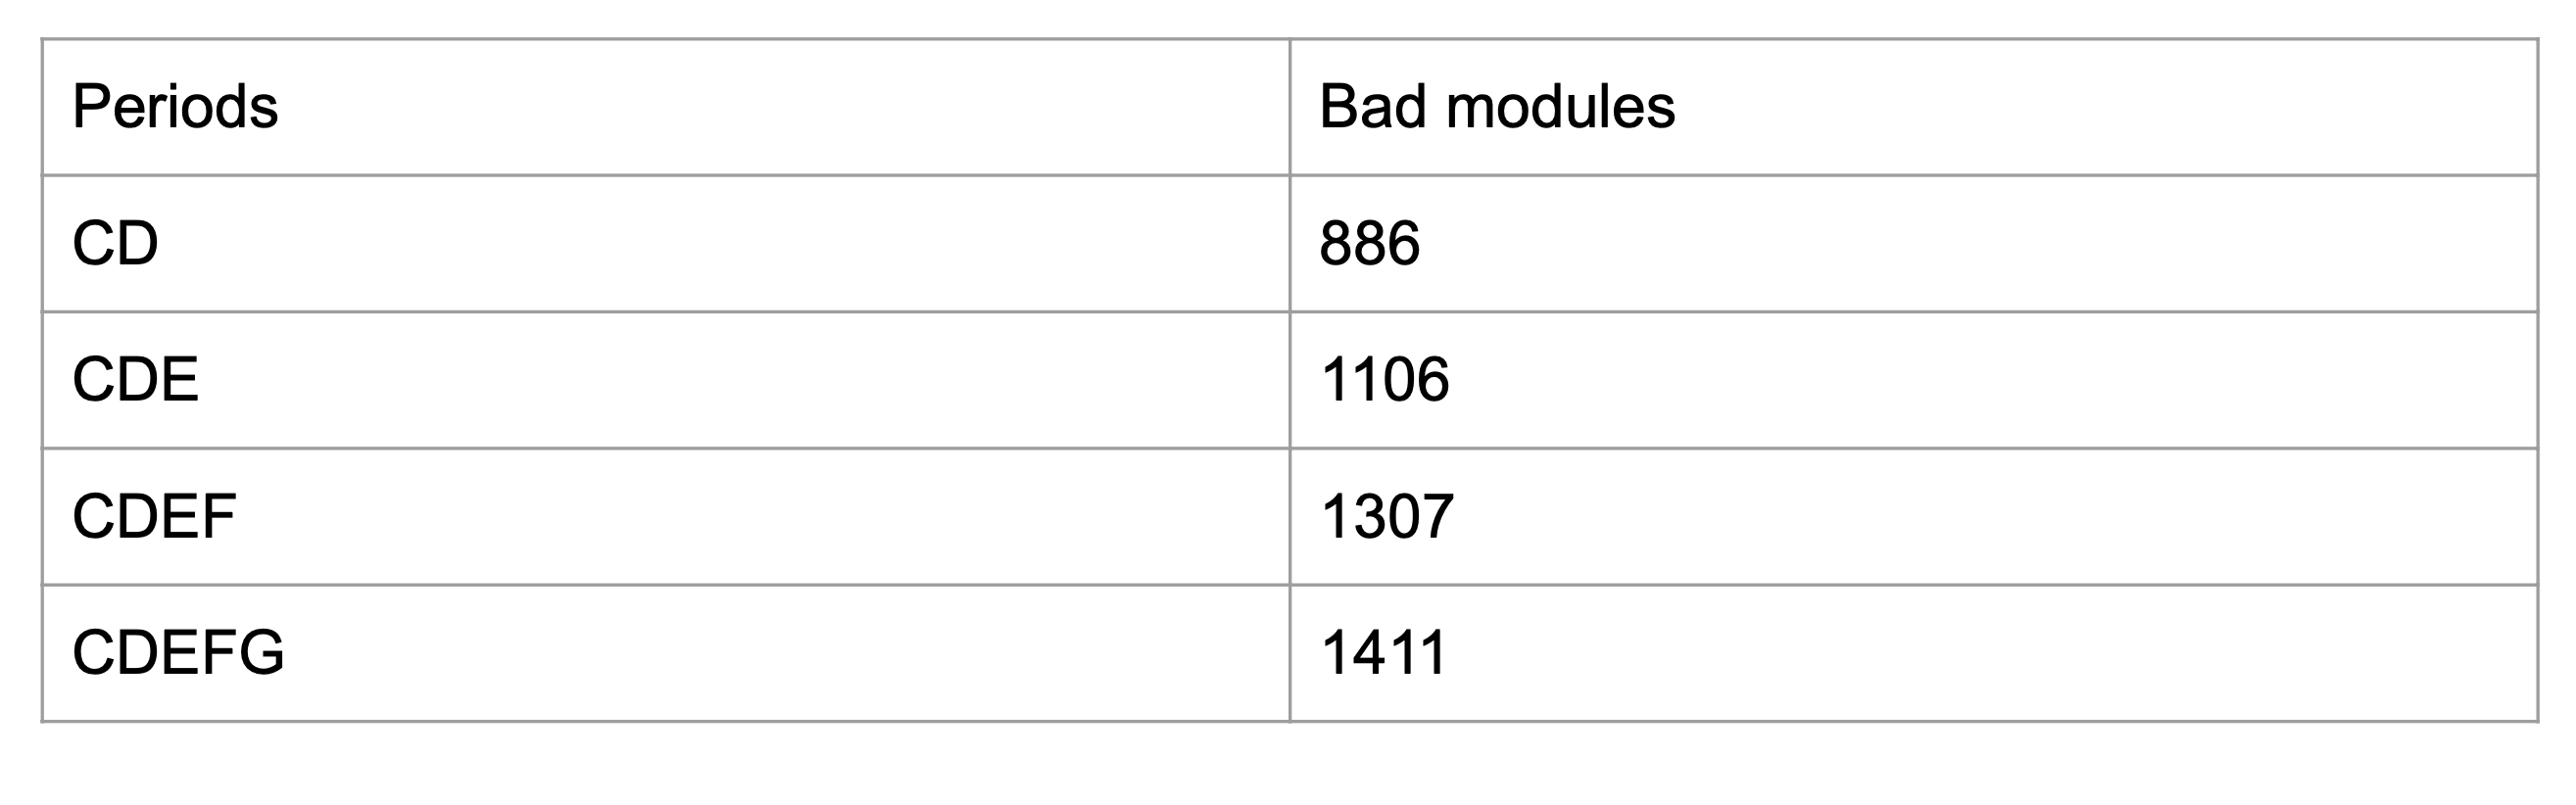
\includegraphics[width=1\textwidth]{ashish_thesis/2022_common_veto.png}
%\caption[2018 CMS luminosity data taking periods.]{%                                                                                                                                             
 % 2022 luminosity data taking periods showing data taking period boundaries and vdM calibration data .
%}
%\label{fig:period_bound}
%\end{figure}

Table \ref{table:12_2022} provides a summary of the number of bad pixel modules identified over different combinations of periods (CD, CDE, CDEF, and CDEFG). The results are achieved using a 4\% rms common module veto list. The table is organized into two columns: 'Periods' and 'Bad Modules'. In the 'Periods' column, various combinations of periods are listed, which denote the time intervals during which the luminosity measurements are conducted. The listed combinations - CD, CDE, CDEF, and CDEFG - indicate that the analysis was done over expanding time frames, starting with periods C and D, then extending to include E, followed by F, and finally G. The 'Bad Modules' column provides the total number of bad or unreliable pixel modules identified across the listed combination of periods. For example, 886 bad modules are found over periods C and D, 1106 bad modules over periods C, D, and E \cite{pas_22}. %\cite{bril2023moduleveto_1}.

\begin{table}[h!]
  \centering
  \caption[Common module veto list]{4\% rms common module veto list. This veto list is created by combining module veto lists of each period.}
\begin{tabular}{ccc}
\textbf{Periods} &  \textbf{Bad Modules} \\
\hline
CD & 886 \\
CDE & 1106 \\
CDEF & 1307 \\
CDEFG & 1411 \\
\end{tabular}
%\caption[Common module veto list]{4\% rms common module veto list. This veto list is created by combining module veto lists of each period.}
\label{table:12_2022}
\end{table}

%\end{comment}

%In a pixel system with 1856 modules, a module veto list filters out unstable modules for luminosity measurement. Only about 10\% pass strict criteria.

%Modules are evaluated based on:

%Stability: Modules with consistent contributions during standard physics runs are retained. Those deviating by initially 5-10\% from the average are excluded. This assessment, rooted in the RMS-to-Mean distribution of cluster counts, is iteratively refined.

%Linearity: Modules are tested for response stability against effective instantaneous luminosity, gauged by the average PCC.

%Using the Run 2022F veto list as a baseline for periods C, D, E, and G, additional unstable or noisy modules are identified and removed, especially during the vdM fill data phase. A summary of exclusions is provided in Table \ref{tab:bad_modules}.

\begin{table}[h]
  \centering
  \caption{Number of bad modules for selection on stability and linearity for various periods.}
\begin{tabular}{lr}
\textbf{Type Or Period/Step} & \textbf{\# of bad modules} \\
\hline
BPIX Layer0 & 96 \\
2022F Stability & 983 \\
2022F Linearity & 1195 \\
2022C Stability & 1364 \\
2022C Linearity & 1484 \\
2022E Stability & 1553 \\
2022E Linearity & 1570 \\
2022G Stability & 1604 \\
2022G Linearity & 1628 \\
2022D Stability & 1653 \\
2022D Linearity & 1677 \\
vdM fill & 1693 \\
\end{tabular}
%\caption{Number of bad modules for selection on stability and linearity for various periods.}
\label{tab:bad_modules}
\end{table}

\end{comment}

%A comprehensive examination of the performance and stability of the pixel detector layers and disks for each lumi section throughout the 2022 data-taking period is shown in Fig. \ref{fig:stabprof_69}. The figure on the left illustrates the proportional contribution to the total detected luminosity from different layers and disks of the pixel detector as a function of lumi section, with only Layer 1 modules vetoed. This plot essentially shows how the luminosity fraction, that is, the relative contribution to the total detected luminosity from each layer and disk, evolves over the course of the data-taking period. The layer 1 module veto indicates that malfunctioning or underperforming modules in Layer 1 of the pixel detector have been systematically excluded from the measurement. The figure on the right presents stability profiles of the pixel detector's layers and disks, taking into account a 4\% RMS common module veto list. %The stability of a module, determined in terms of its consistent response to incoming particles and reliability in data recording, is crucial for accurate measurements. The "4\% RMS common module veto list" refers to modules that have been omitted from data analysis due to their performance deviation - in terms of variability or RMS - exceeding 4\% from an expected value.
  
\begin{figure}[!htp]
  \centering
  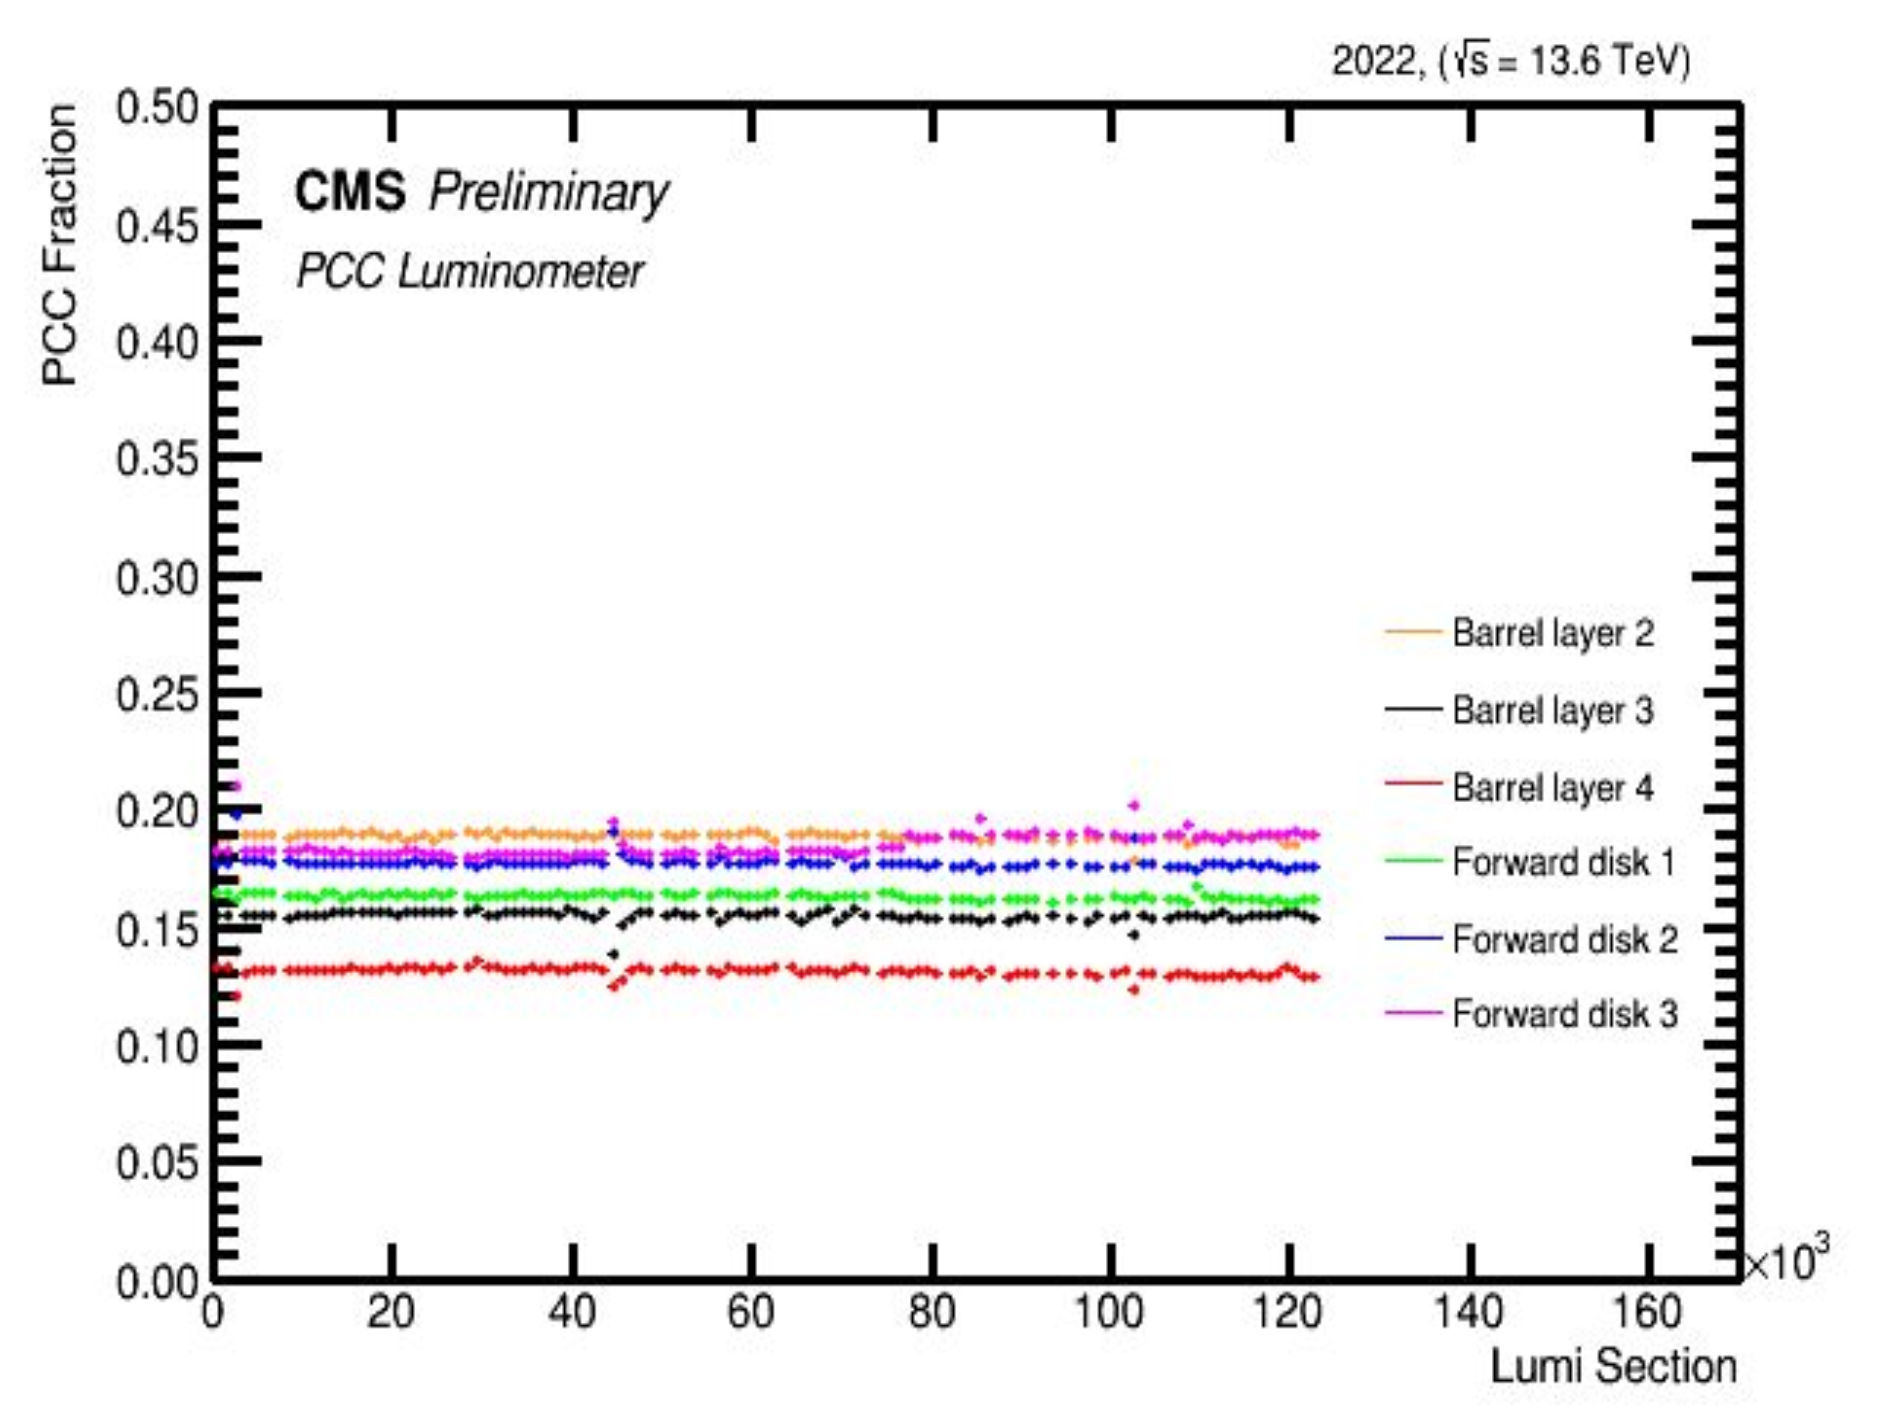
\includegraphics[width=0.7\textwidth]{ashish_thesis/PCC_stability_2022_L0veto_4.png}
  \caption[Luminosity fractions w/o layer 0 modules]{Luminosity fraction of pixel detector for various layers and disks as a function of lumi section for the entire 2022 data with all Layer 0 modules vetoed.}
  \label{fig:stabprof_69a}
\end{figure}


\begin{figure}[!htp]
  \centering
  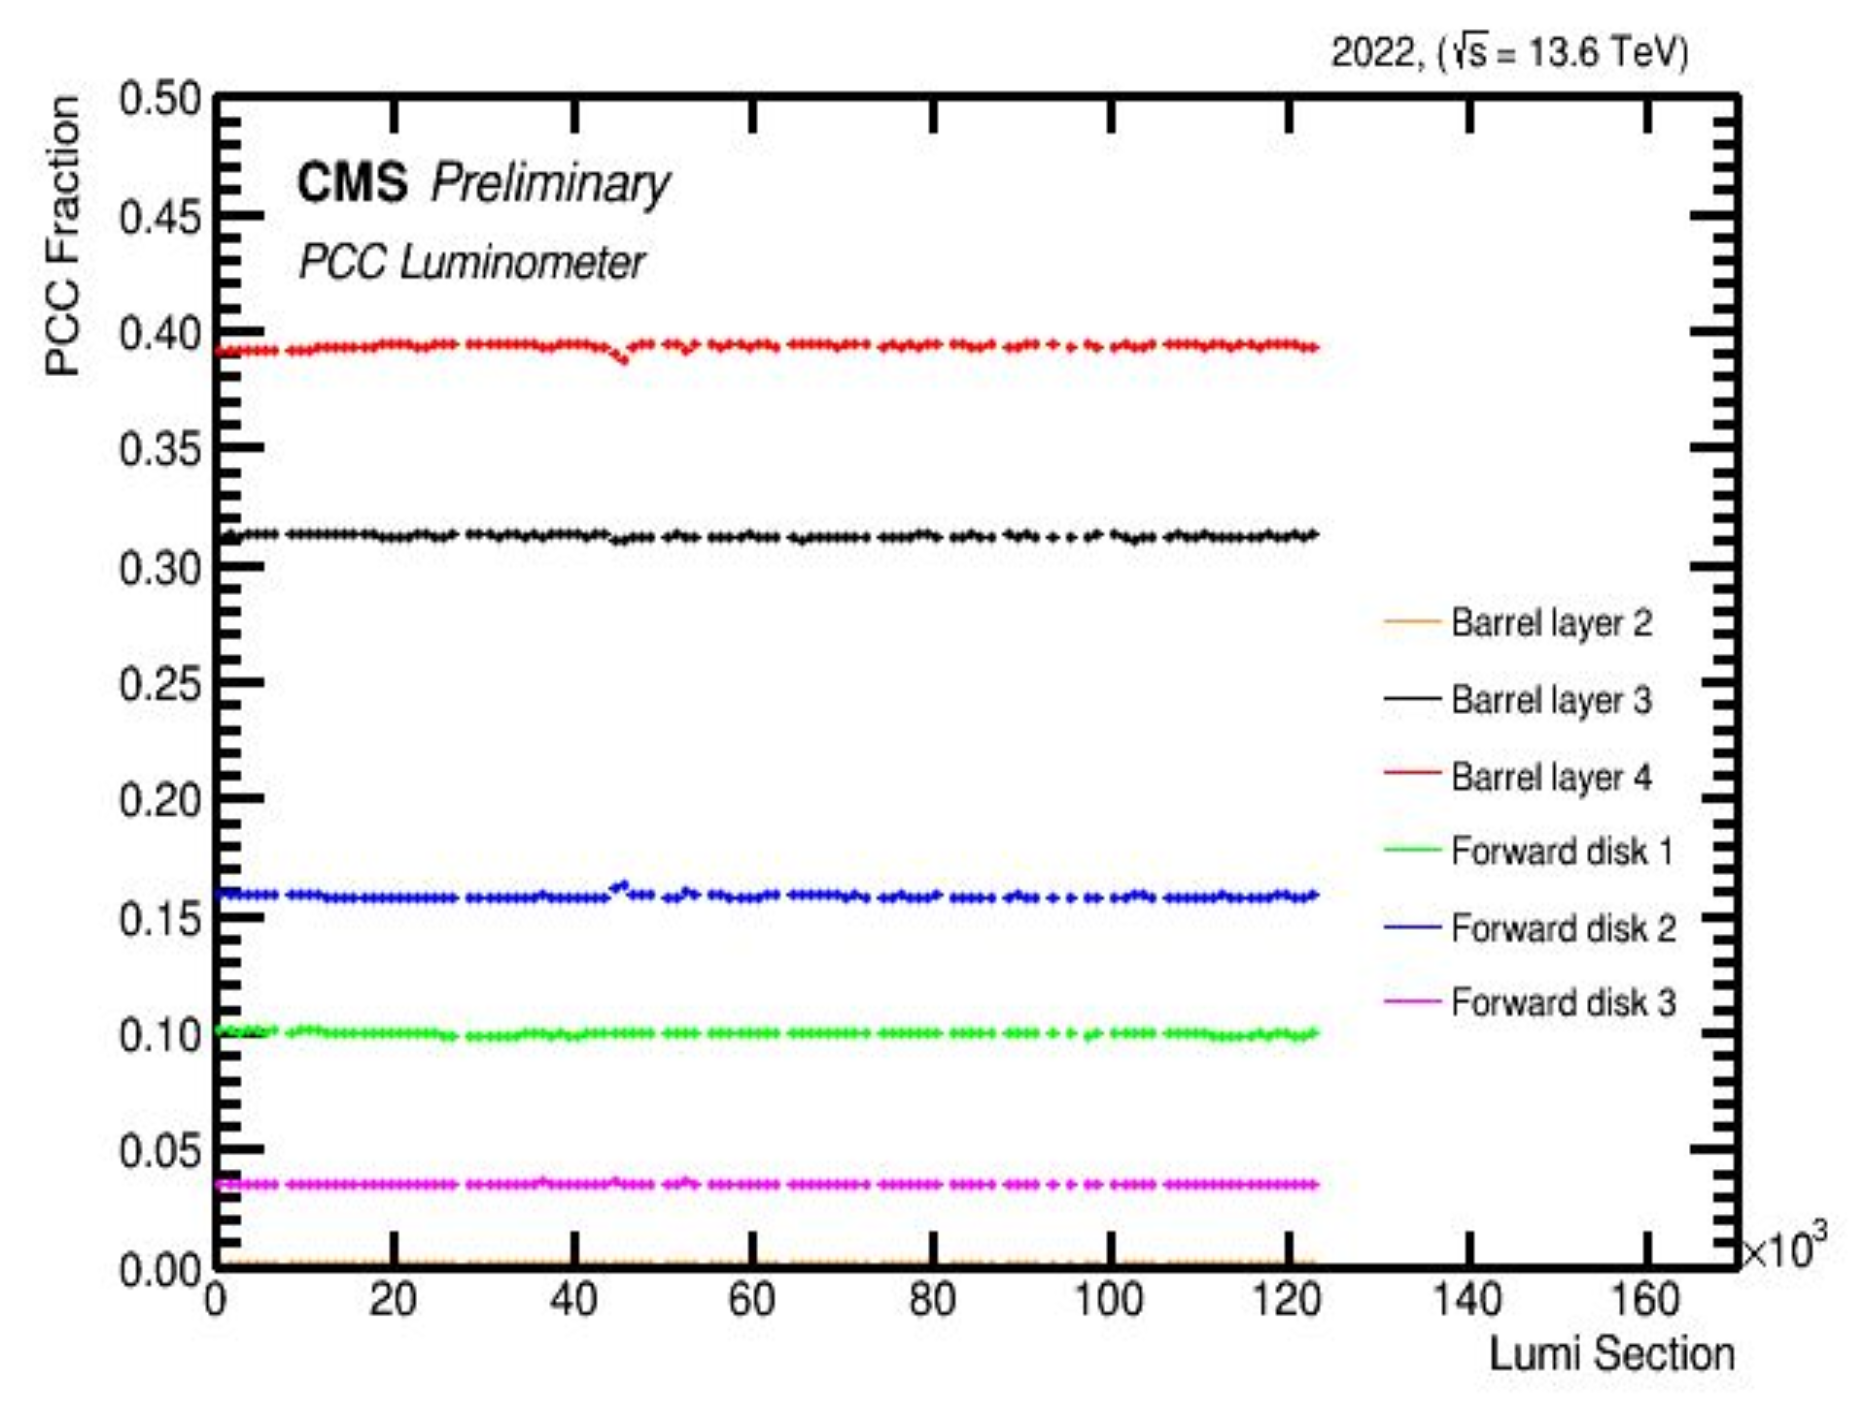
\includegraphics[width=0.7\textwidth]{ashish_thesis/2022_pcc_stability_2.png}
  \caption[Stability profiles for final veto]{Stability profiles of pixel detector layers and disk modules for the final module veto list.}
  \label{fig:stabprof_69b}
\end{figure}


\begin{comment}
  
\begin{figure}[!htp]
  \centering
  \begin{subfigure}[b]{0.49\textwidth}
    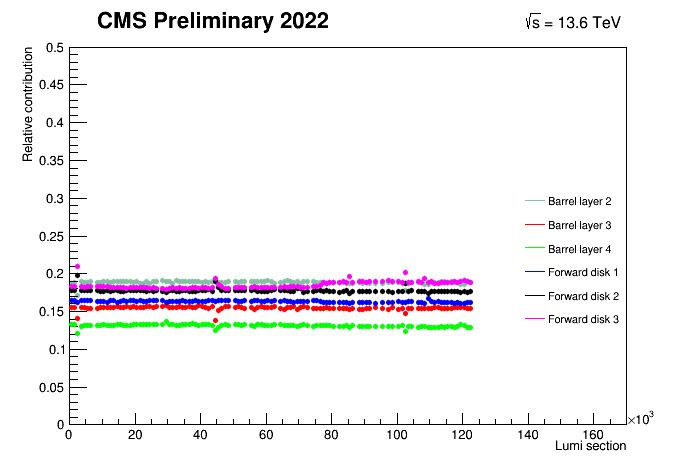
\includegraphics[width=\textwidth]{ashish_thesis/PCC_stability_2022_L0veto.png}
    %\caption{Image 1}                                                                                                                                                                           
  \end{subfigure}
  \hfill % or \hspace{5mm} for a specific horizontal space                                                                                                                                      
  \begin{subfigure}[b]{0.49\textwidth}
    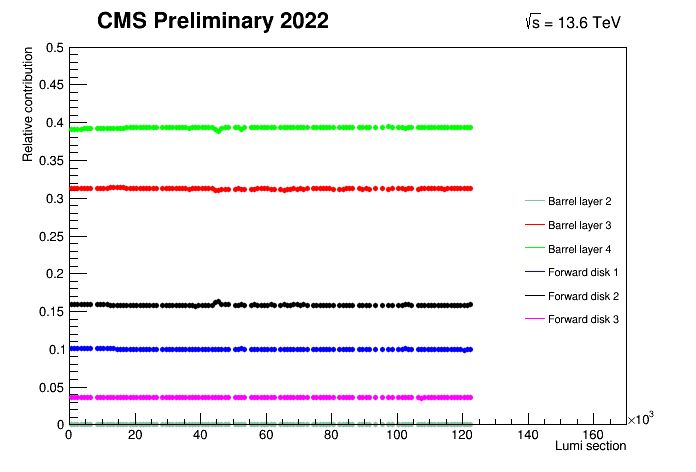
\includegraphics[width=\textwidth]{ashish_thesis/2022_pcc_stability.png}
    %\caption{Image 2}                                                                                                                                                                           
  \end{subfigure}
  \caption[Pixel detector stability plots without and with veto list]{Left: Luminosity fraction of pixel detector for various layer and disks as a function of lumi section for the entire 2022 data  with all Layer 0 modules vetoed. Right: Stability profiles of pixel detector layer and disk modules for the final module veto list.}
  \label{fig:stabprof_69}
\end{figure}

\end{comment}

\newpage
\section{vdM calibration results}

The vdM calibration involves varying the position of the colliding proton beams horizontally and vertically and observing the changes in the event rate resulting from these shifts as a function of beam separation. This procedure allows us to determine the overlap integral of the beam profiles, which is an essential part of the absolute luminosity calculation. In the context of PCC, the event rate corresponds to the number of pixel clusters detected per unit time. Therefore, by observing how this rate changes with the beam positions, the calibration constant of the PCC luminometer can be determined. % the efficiency and response of the pixel detector.

%The key steps of the vdM calibration procedure: Beam Separation Scans: Two beams are made to collide, and the number of collisions (events) is counted. The beam separation in either the horizontal or vertical direction is then progressively increased, and the change in the number of events is measured. This procedure allows for the determination of the spatial distribution of each beam, referred to as the beam profile. Fitting of Scan Data: The beam profiles obtained from the scans are then used to fit a function to the event rate as a function of beam separation. The maximum of this function gives the event rate when the beams are perfectly overlapped. Calculation of Luminosity: The luminosity is directly proportional to the event rate at perfect overlap and inversely proportional to the area of the beam profiles. Using these relationships, the absolute luminosity can be calculated. Calibration of the Detector: The calibration constant or visible cross section obtained from absolute luminosity and peak rate during vdM calibration is then used to calibrate the detector.

The vdM scan was performed in November 2022, during the LHC fills 8379 and 8381. In fill 8381 on 10–11 Nov 2022, data was collected when 144 paired bunches of particles were colliding, with additional unpaired bunches also present. Various scan pairs were conducted, including four vdM scans, two Beam Imaging (BI) scans, and one length scale scan. Each of these scans consists of two examinations in the x and y transverse planes. In the vdM scan, beams were separated by a distance correlating to six times transverse beam size and then moved across each other in 25 steps. Each step lasted 30 seconds and moved the beams by half of their transverse size. For the BI scans, one beam remained fixed while the other moved in 19 steps, over a distance of up to 4.5 times its transverse size. The length scale scan involved beams being separated by a constant distance and moved in both directions in five steps. The scan program during fill 8381 is shown in Fig. \ref{fig:2022_vdM_program}.

\begin{figure}[!htp]
\centering
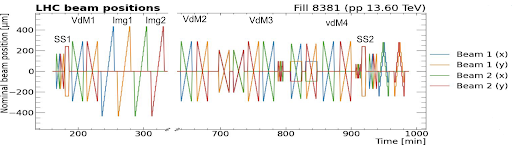
\includegraphics[width=1\textwidth]{ashish_thesis/2022_vdM.png}
\caption[2022 vdM program]{%                                                                                                                                             
  2022 vdM calibration program. In LHC fill 8381, proton beam positions were recorded, including four vdM scans, two BI scans, one LS scan, and two SS periods \cite{pas_22}.
}
\label{fig:2022_vdM_program}
\end{figure}

%On November 10, 2022, during the LHC fill 8370, 58 paired bunches were colliding at the CMS Interaction Point (IP), with 12 extra unpaired bunches in each beam. An extra length scale scan pair was conducted during this fill. %Moreover, a secondary scan program occurred during LHC fill 8178 from September 24-26, 2022, focusing on data collection for the LHCf experiment. At the CMS IP, 144 bunch pairs were colliding with two additional unpaired bunches in each beam. %Several scans took place, but only results from three length scale scan pairs are mentioned here, one of which had nine steps per direction rather than the typical five.

The result of the calibration is described in
%Normalized Rates and Resulting Fitted Double Gaussian Scan Curves for Single Bunch in X and Y Directions:
Figure \ref{fig:period_bound_50} which depicts how the detected event rate varies as the beams are scanned across each other in the horizontal (X) and vertical (Y) directions.The rates have been fitted to a double Gaussian curve, which reflects the bell-shaped spatial distribution of the proton bunches. The peaks of these curves correspond to the maximum event rate, which occurs when the beams are perfectly overlapped. The width of the curve gives an indication of the spread of the beam in the respective direction. In the final analysis. a floating constant is used in the fit for the background because the background from the SS1 and SS2 give inconsistent values as shown in Table \ref{table:side_by_side}.

\begin{table}[!htp]
  \centering
  \caption[2022 PCC background rate]{PCC background rate for five BCIDs during super separation scans 1 and 2. Average PCC background rate is calculated by averaging over all five BCIDs.}
    \begin{minipage}{0.45\textwidth}
        \centering
        \begin{tabular}{ccc}
          \hline
            \multicolumn{3}{|c|}{SS 1} \\
            \hline
            BCID & Mean & SEM \\
            \hline
            282 & 0.03917 & 0.00147 \\
            822 & 0.03896 & 0.00130 \\
            2944 & 0.03979 & 0.00145 \\
            3123 & 0.03788 & 0.00132 \\
            3302 & 0.03931 & 0.00130 \\
        \end{tabular}
        \subcaption{SS1_{avg}= 0.0390 +- 0.000613}
    \end{minipage}%                                                                                                                                                                                                  
    \hfill
    \begin{minipage}{0.45\textwidth}
        \centering
        \begin{tabular}{ccc}
            \hline
            \multicolumn{3}{|c|}{SS 2} \\
            \hline
            BCID & Mean & SEM \\
            \hline
            282 & 0.07682 & 0.00128 \\
            822 & 0.077513 & 0.00137 \\
            2944 & 0.082114 & 0.00178 \\
            3123 & 0.075385 & 0.00127 \\
            3302 & 0.077605 & 0.00139 \\
        \end{tabular}
        \subcaption{SS2_{avg}= 0.077902 -+ 0.00060436}
    \end{minipage}
    %\caption{PCC background rate for five BCIDs during super separation scans 1 and 2. Average PCC background rate is calculated by averaging over all five BCIDs.}                                                 
    \label{table:side_by_side}
\end{table}

%Background subtraction and beam corrections have been applied to the raw data to account for noise.
%Chi2/ndof for all vdM and Imaging Scans:
%Figure \ref{fig:period_bound_51} provide an indication of the quality of the fits to the scan data.
The $\chi^2$ statistic measures the discrepancy between the observed event rates and the values predicted by the double Gaussian fit, while ndof (number of degrees of freedom) accounts for the complexity of the fit. A value of  $\chi^2$/ndof close to 1 can be seen in the statistics box which signifies a good fit. The variation of $\chi^2$/ndof across scans is shown in Fig. \ref{fig:period_bound_510}. From this plot, we can observe that the average fit quality of the data to the model, as measured by the chi-squared per degree of freedom (chi2/ndof), is slightly above the ideal value of 1, with a mean of approximately 1.55. This suggests that the model fits the data reasonably well overall, but there may be some systematic deviation. The consistency of fit quality across different scans, both X and Y, indicates that no significant discrepancy exists between these two scanning directions within the range of values presented.  The change in beam overlap width across scans is shown in Fig. \ref{fig:period_bound_520}. The plot reveals an asymmetry in beam overlap widths, with the X-Scans showing higher CapSigma values than the Y-Scans in all scans, indicating a larger beam width along the X-axis. The Y-Scans exhibit narrower and more uniform widths, suggesting a more stable overlap along the Y-axis. This consistent difference in the overlap widths between the X and Y scans is evident across various vdM and beam imaging scans.The PCC visible cross section is 1076 $\pm$ 0.9 (stat) mb. The bunch to bunch variation and scan to scan variation of the PCC visible cross section is shown in Fig. \ref{fig:period_bound_99} and Fig. \ref{fig:period_bound_105} \cite{pas_22}. %\cite{bril2023vdmrecalibration}.

%Beam Overlap Widths for each vdM and Imaging Scans:
%Figure \ref{fig:period_bound_52} show the beam overlap widths, or the widths of the double gaussian fit, for each scan. %The overlap width essentially gives the size of the beam at the interaction point and is used to calculate the absolute luminosity. Comparison of these widths across different scans can reveal variations in the beam size over time.
%Figure \ref{fig:period_bound_53} show the maximum event rate for each scan, which corresponds to the peak of the double gaussian fit. This peak rate is achieved when the beams are perfectly overlapped.

\begin{figure}[!htp]
\centering
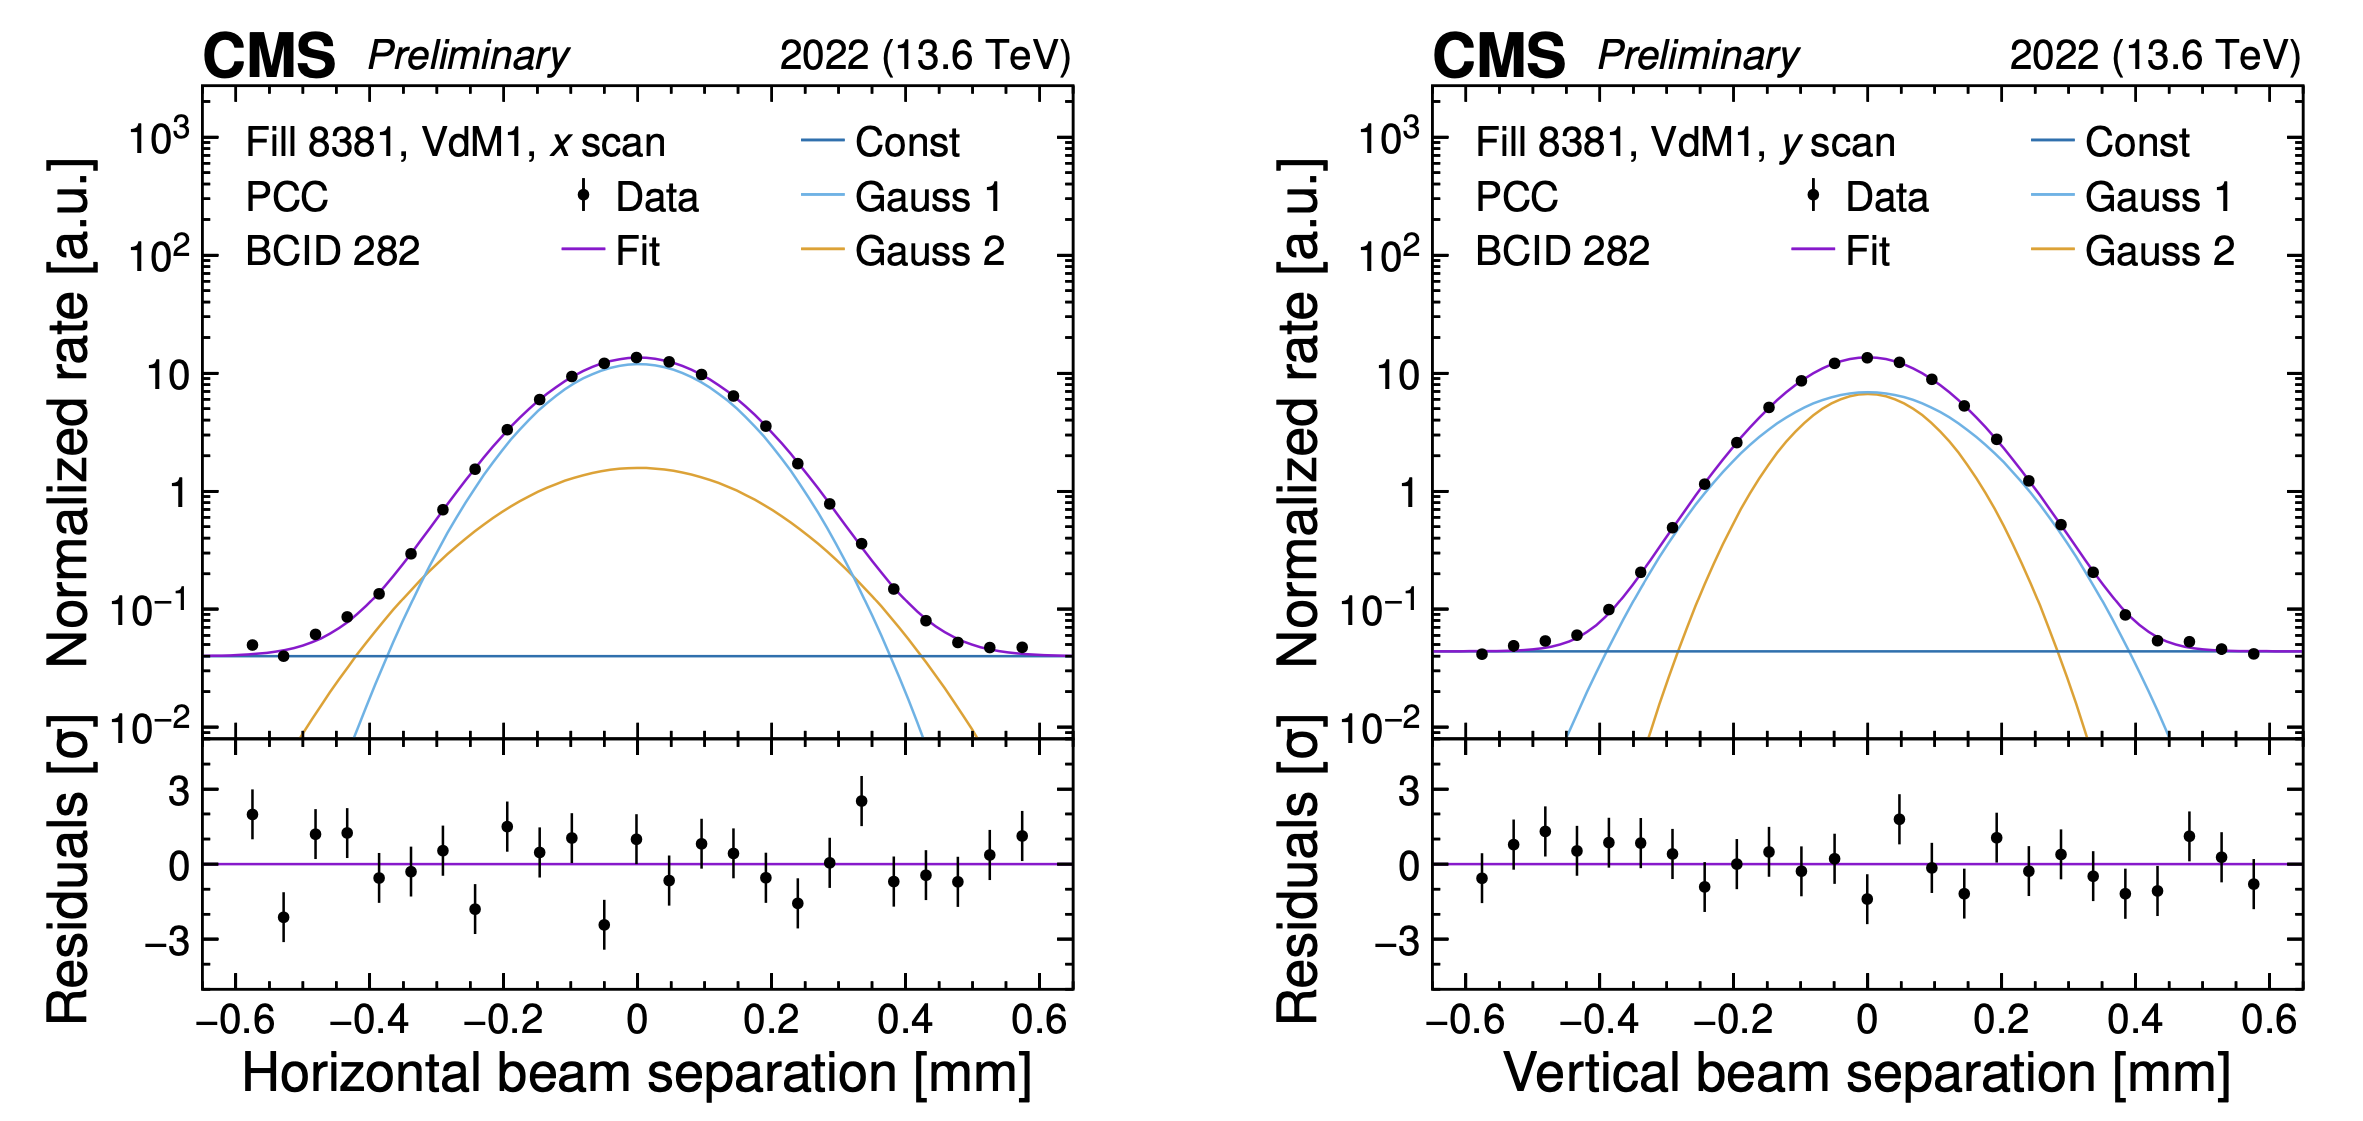
\includegraphics[width=1\textwidth]{ashish_thesis/2022_PCC_vdM_fit_new.png}
\caption[2022 PCC vdM fit]{%                                                                                                                                              
  Rates and the resulting fitted double Gaussian scan curves as a function of the beam separation for a single bunch (BCID 282) as recorded by PCC for a vdM1 scan in the x (left) and y direction (right). Beam corrections have been applied to the raw data before the fit.
}
\label{fig:period_bound_50}
\end{figure}

\begin{figure}[!htp]
\centering
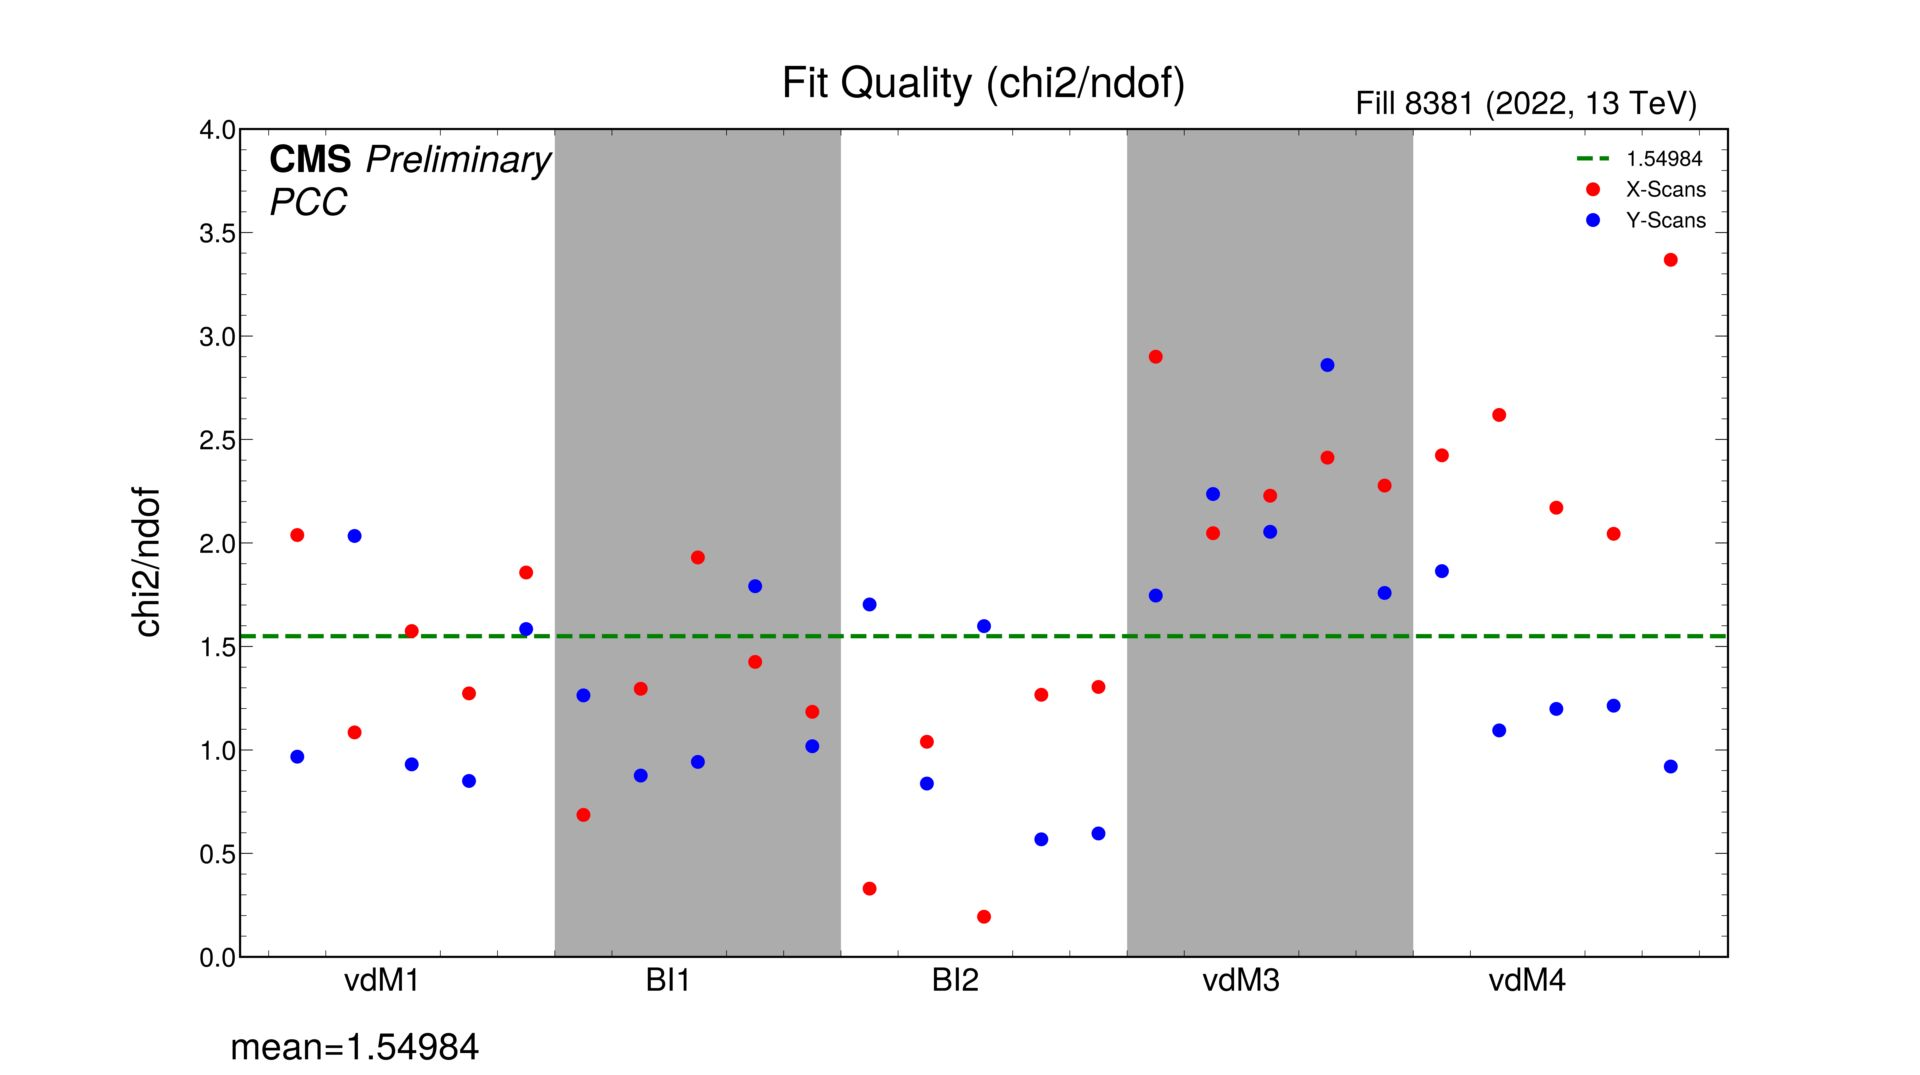
\includegraphics[width=1\textwidth]{ashish_thesis/DGConst_chi2.jpeg}
\caption{%                                                                                                                                                                  
  $\chi^2$/ndof for all vdM and imaging scans.
}
\label{fig:period_bound_510}
\end{figure}


\begin{figure}[!htp]
\centering
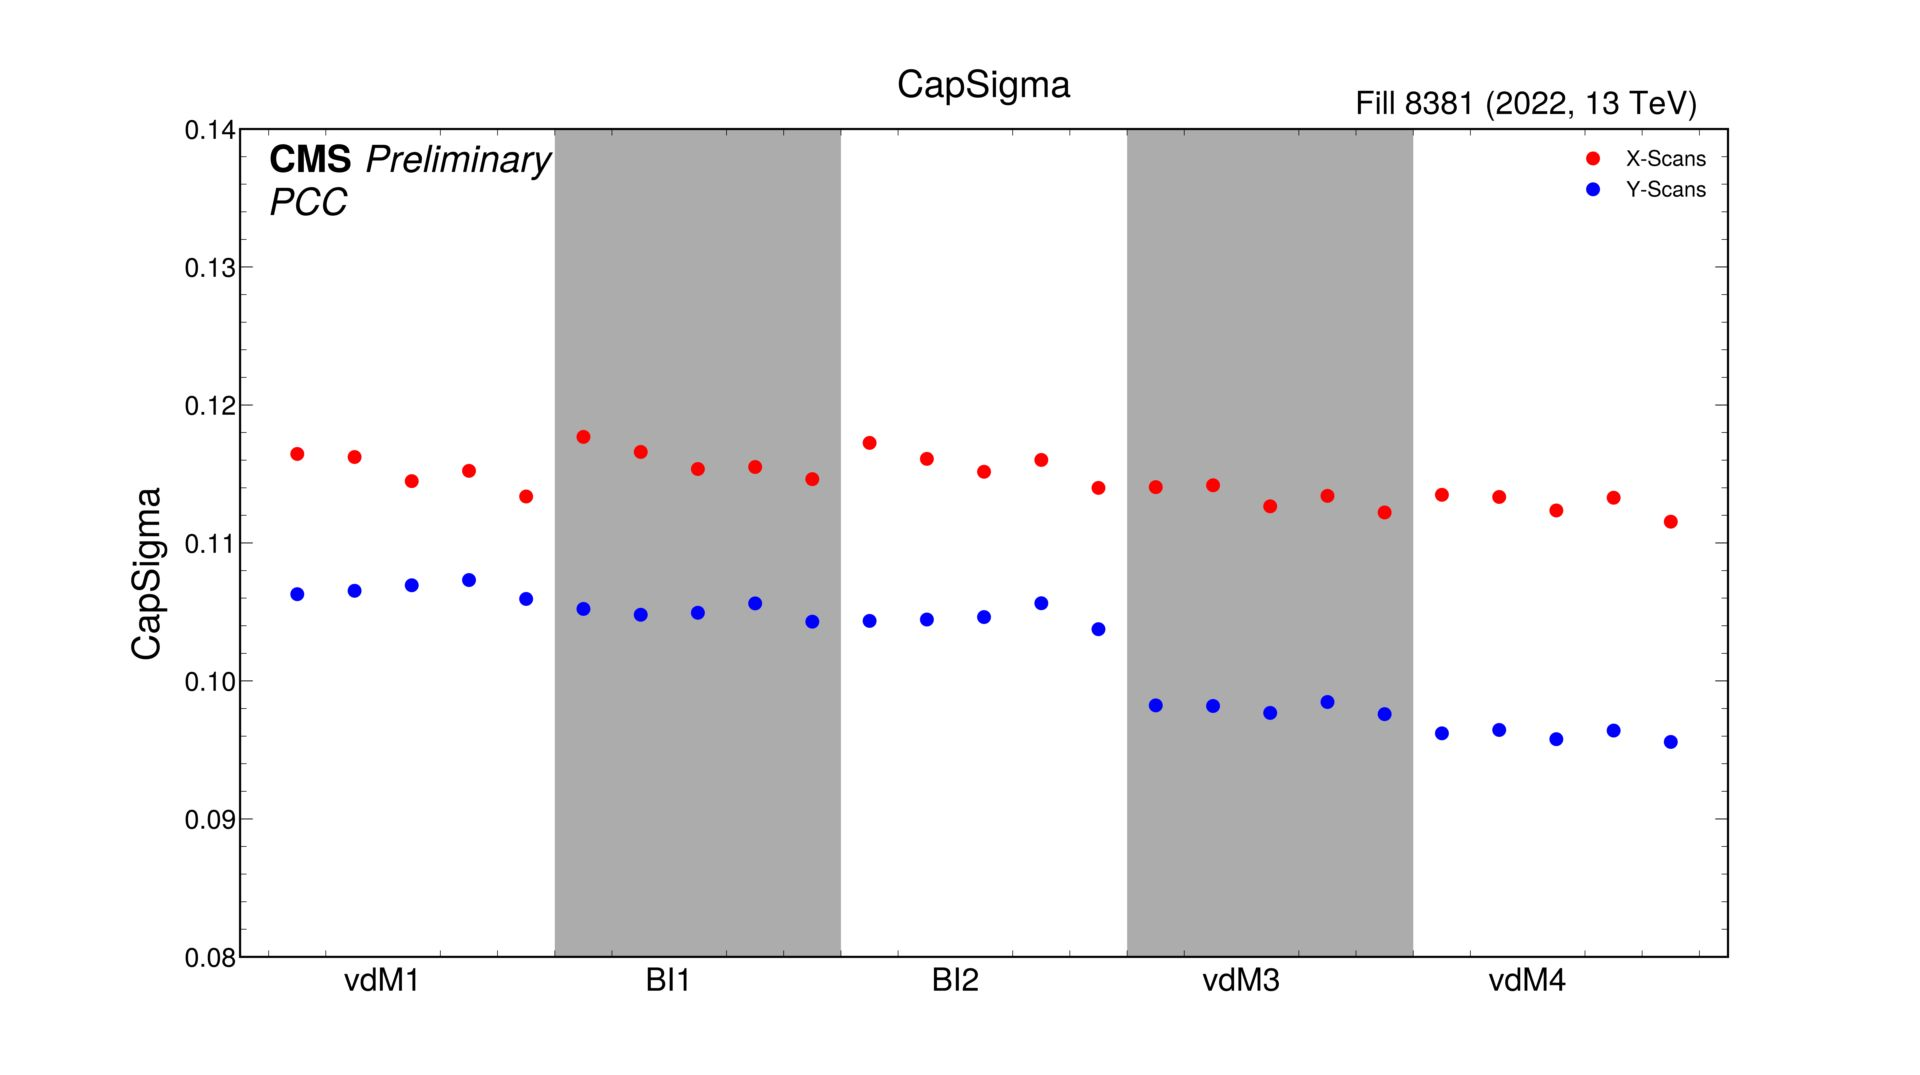
\includegraphics[width=1\textwidth]{ashish_thesis/DGConst_CapSigma.jpeg}
\caption[Beam overlap widths]{%                                                                                                                                            
                                                                                                                                                                         
  Beam overlap widths for each vdM and imaging scans.
}
\label{fig:period_bound_520}
\end{figure}


\begin{comment}
  
\begin{figure}[!htp]
\centering
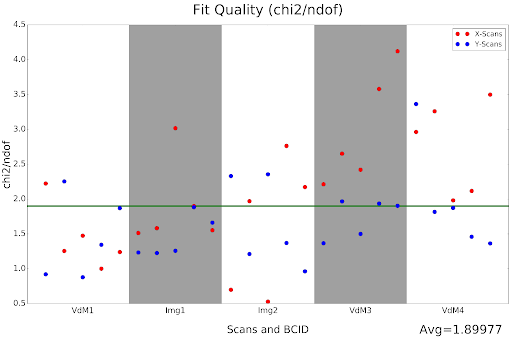
\includegraphics[width=0.6\textwidth]{ashish_thesis/2022_vdM_fit_quality-png.png}
\caption{%                                                                                                                                             
  $\chi^2$/ndof for all vdM and imaging scans.
}
\label{fig:period_bound_51}
\end{figure}


\begin{figure}[!htp]
\centering
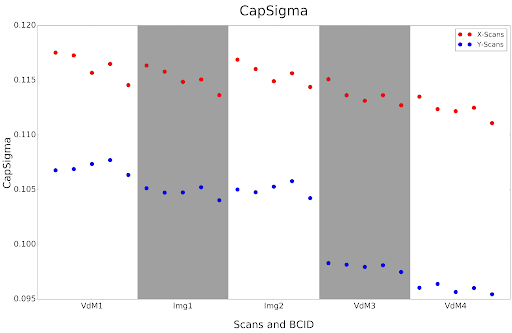
\includegraphics[width=0.6\textwidth]{ashish_thesis/2022_capsigma.png}
\caption[Beam overlap widths]{%
  Beam overlap widths for each vdM and imaging scans.
}
\label{fig:period_bound_52}
\end{figure}

\begin{figure}[!htp]
\centering
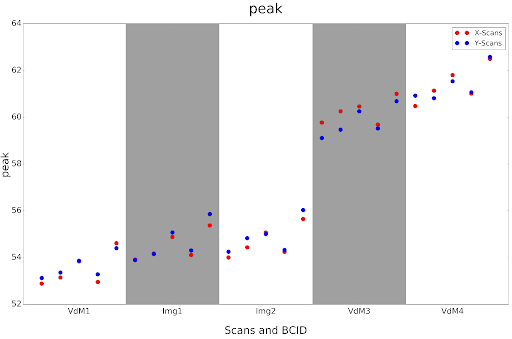
\includegraphics[width=0.6\textwidth]{ashish_thesis/2022_peak.png}
\caption[Peak PCC rate]{%                                                                                                                                             
  Peak PCC rate for each vdM and imaging scans.
}
\label{fig:period_bound_53}
\end{figure}

\end{comment}

%PCC visible cross section is 1076 $\pm$ 0.9 (stat) mb as shown in Fig. \ref{fig:period_bound_105}.

\begin{figure}[!htp]
\centering
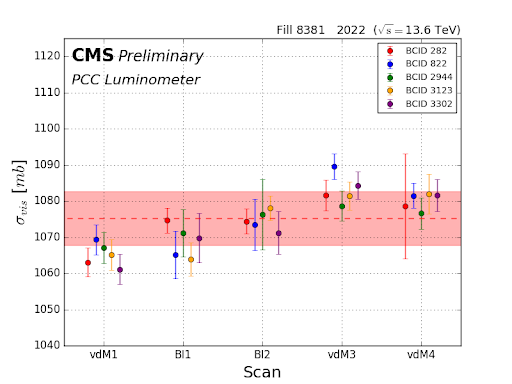
\includegraphics[width=0.8\textwidth]{ashish_thesis/2022_sigma_vis_btob_variation.png}
\caption[$\sigma_{vis}$ bunch variation]{%                                                                                                                                                        
  Bunch to bunch variation of PCC visible cross section where the red line is the average value. Red band depicts the $\pm$ one RMS of the values.
}
\label{fig:period_bound_99}
\end{figure}

\begin{figure}[!htp]
\centering
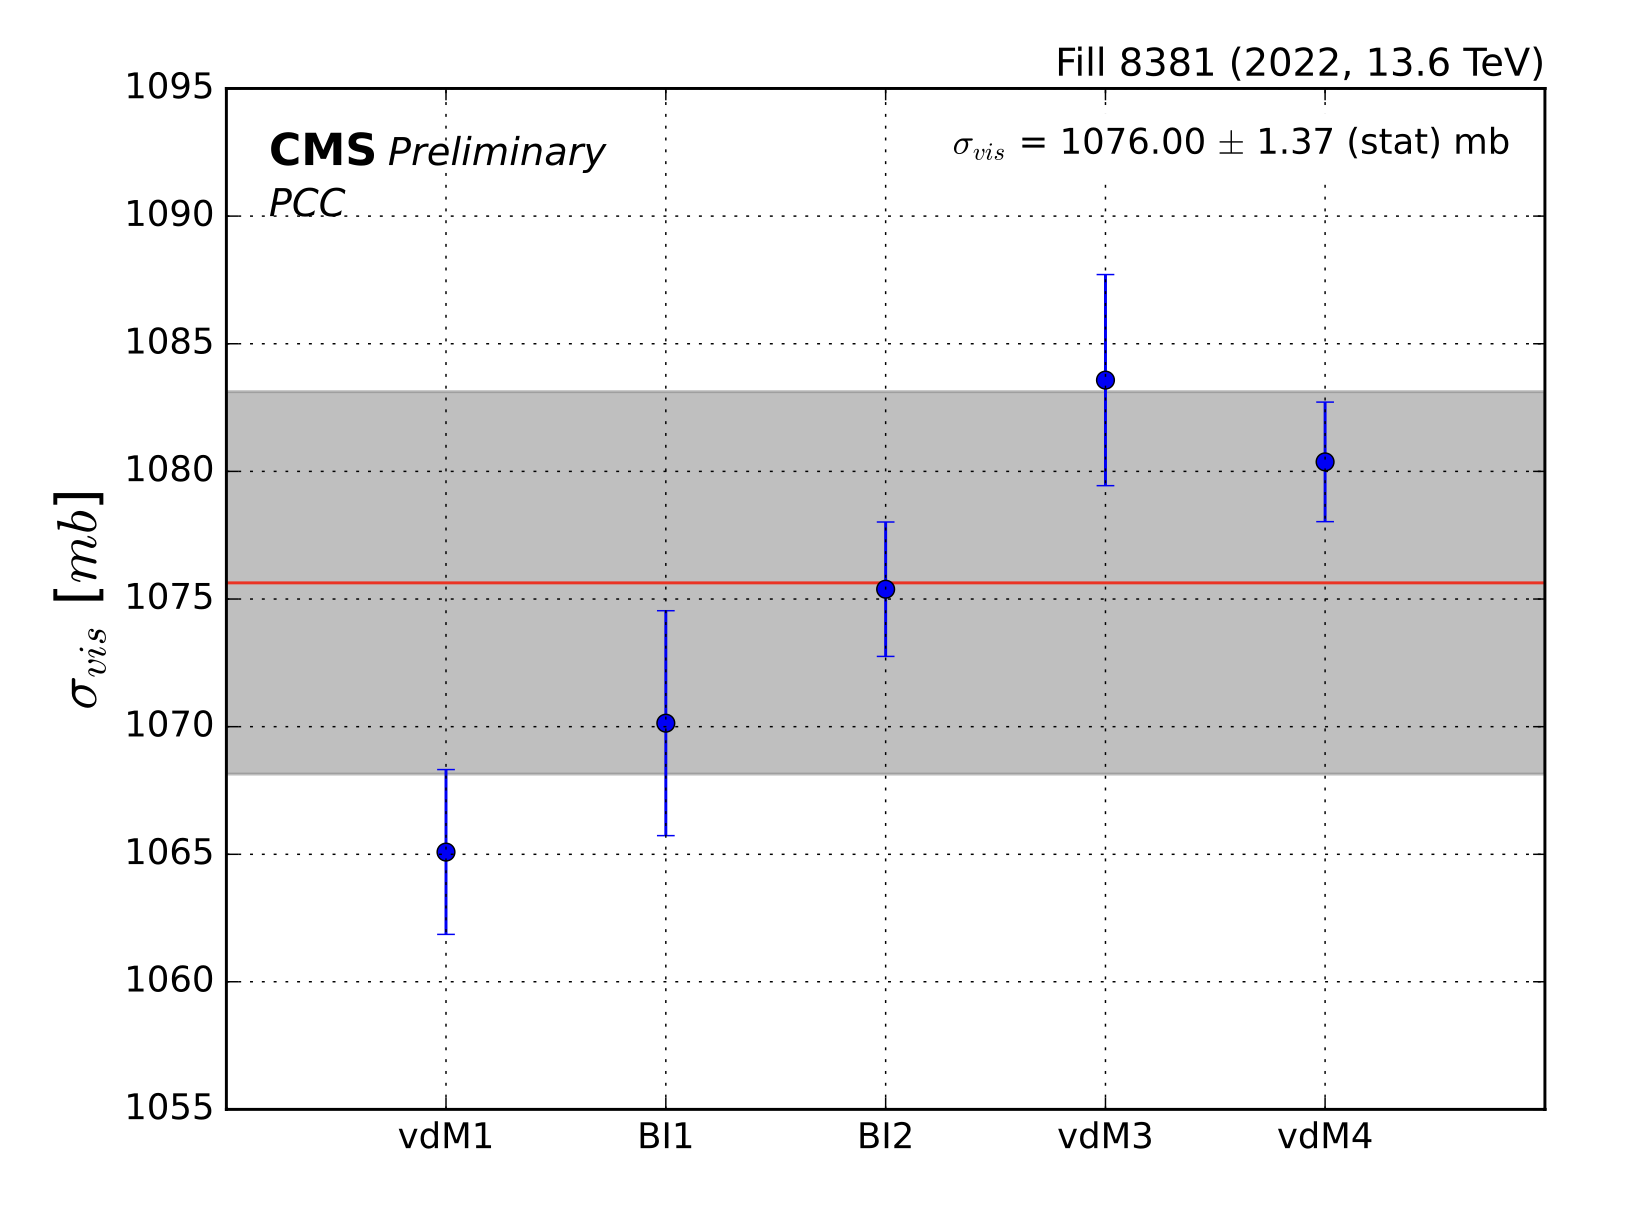
\includegraphics[width=0.8\textwidth]{ashish_thesis/2022_PCC_sigmavis_per_scan_new.png}
\caption[2022 PCC visible cross section]{%                                                                                                                                                                               
  Visible cross section per scan where red line shows the average value. Red band depicts the $\pm$ one RMS of the values.
}
\label{fig:period_bound_105}
\end{figure}

\newpage
\section{Luminosity for physics fills}

The fill cycle in Run 3 includes a leveling part in order to control the very high pileup achieved with upgraded LHC beam optics. The fill luminosity profile for fill 8395 during 2022 data taking is shown in Fig. \ref{fig:period_bound_111}. This fill consists of

\begin{itemize}
  
\item 2450 colliding bunches

\item 2600 lumi sections

\item peak luminosity of $19000 \text{Hz} / \text{ub}$

%\item minimum luminosity of 8.5 \times 10^{33} \, \text{cm}^{-2} \, \text{s}^{-1}

\end{itemize}

\begin{figure}[H]
\centering
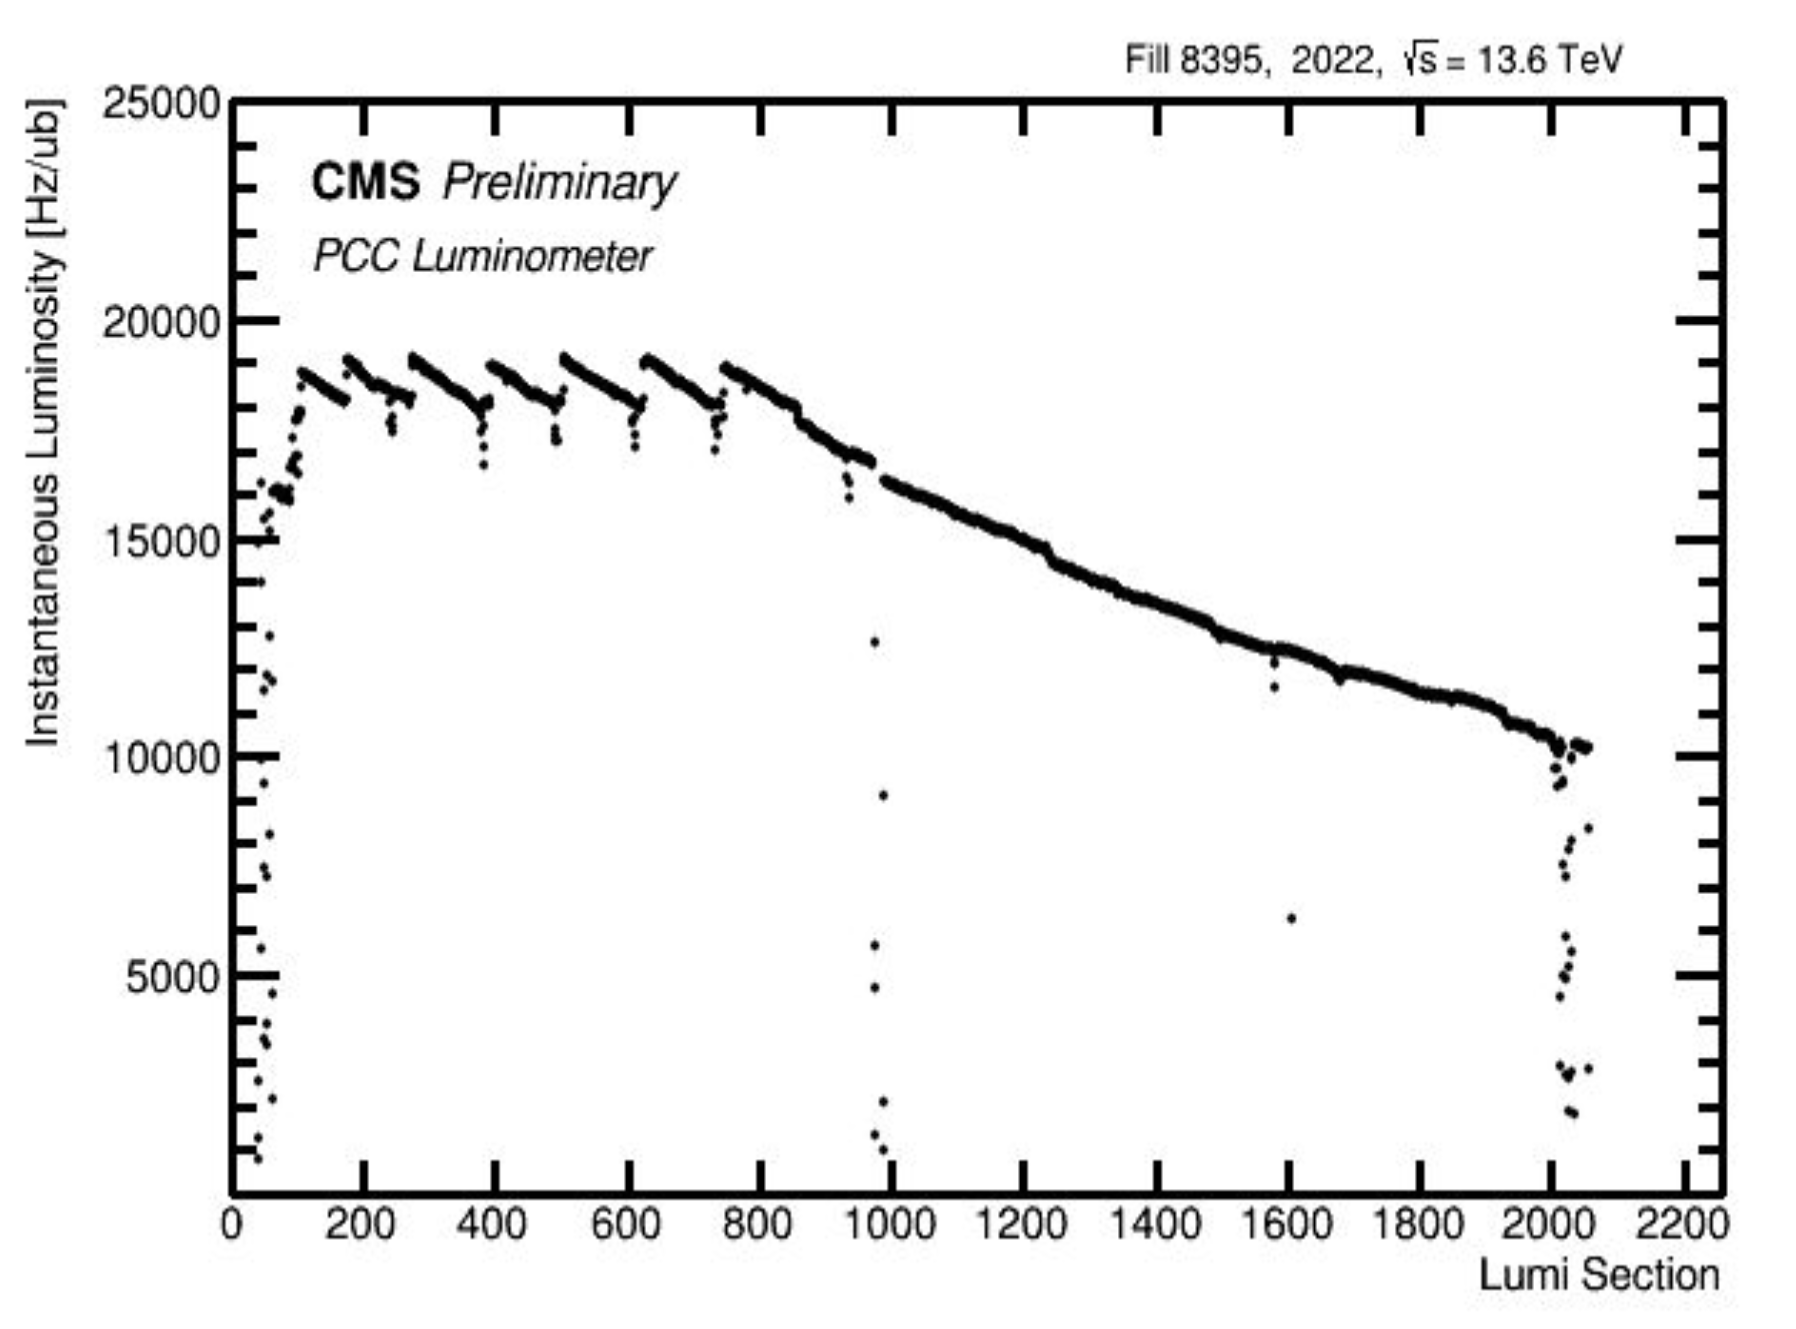
\includegraphics[width=1\textwidth]{ashish_thesis/Fill_profile_8274_1.png}
\caption[Fill 8274 luminosity profile]{%                                                                                                                                                                                         
  PCC luminosity profile for fill 8395.
}
\label{fig:period_bound_111}
\end{figure}

%\newpage
\subsection{Afterglow background corrections}

%Figure \ref{fig:period_bound_44} and  \ref{fig:period_bound_45} describe the residuals of the PCC afterglow correction model fit as a function of instantaneous luminosity. The afterglow effect in PCC luminosity measurement refers to the lingering response of the detector to a previous collision event, which could lead to a systematic overestimate of the luminosity in subsequent bunch crossings.

Corrections are introduced to the PCC measurement to mitigate background effects. The considered background contributions for physics fills are:

\begin{itemize}
    %\item \textbf{Pedestal}: Represents a consistent noise in the pixel cluster count.
    
    \item \textbf{Afterglow (Out-of-time counts)}:
    \begin{itemize}
        \item \textbf{Type 1}: Activations from the preceding bunch's pixels. Rectified by observing subsequent bunch clusters.
        
        \item \textbf{Type 2}: Due to the detector's material activation, modeled using an exponential decay function for non-colliding bunches post-train.
    \end{itemize}
\end{itemize}

Both pedestal and type-1 parameters are determined in each 50 LS blocks.

Type-2 parameters, derived from a preceding study using Random trigger data, are presumed to remain constant during the year. The fitting template is given by:
\begin{equation}
F(x) = \Sigma_{k=0}^{N_{bcid}} N_k \left[(x-k==0)+\alpha\cdot(x-k==1)+A \cdot e^{-\tau\cdot(x-k-1)}(x-k>=1) \right]
\end{equation}
with $k$ denoting the colliding bunch crossing and $x$ indicating the histogram bin. 2022 PCC afterglow model uses run number 361957 for fitting the type 1 and type 2 afterglow effect in the PCC raw data as shown in Fig. \ref{fig:period_bound_101}. The model consists of a parameter for type 1 afterglow correction and an exponentially decaying function with two parameters, amplitude and decay width, to model type 2 afterglow correction. The fit function
%correcton and exponentially decaying function with two parameters amplitude and decay width to model type 2 afterglow correction. Fit function
is summed over all bunch crossings. Fit perfomed for 4 wagon train is shown in Fig.  \ref{fig:period_bound_102} in run 361957 to compute type 2 afterglow amplitude and decay width. The values obtained for type 2 afterglow amplitude and decay parameters are 0.0008406 and 0.01047 respectively \cite{pas_22}. %\cite{bril2023afterglow}.
%as shown in Table. \ref{table:trains_data}.

%Type 1 Afterglow Effect: This effect pertains to the first empty bunch crossing immediately following a colliding bunch. Fig. \ref{fig:period_bound_44} visualizes the Type 1 residual as a function of instantaneous luminosity. The residual fraction is computed as the ratio of the luminosity measured in the first empty bunch immediately following a colliding bunch to the luminosity of the colliding bunch itself. If the afterglow effect is significant, this ratio will be higher than expected, indicating that some of the signals attributed to the empty bunch actually originate from the preceding colliding bunch due to the afterglow effect. The objective of the Type 1 correction is to account for this lingering response and adjust the measured luminosity appropriately.
%Type 2 Afterglow Effect: This effect pertains to the second and following empty bunch crossings after a colliding bunch. Fig. \ref{fig:period_bound_45} illustrates the Type 2 residual as a function of instantaneous luminosity. These residuals are calculated similarly to Type 1, but they use the luminosity measurements from the second and subsequent empty bunches after a colliding bunch. The ratio of these measurements to the luminosity of the colliding bunch provides an estimate of the extent of the afterglow effect beyond the immediate aftermath of a collision. The aim of the Type 2 correction is to account for any persistent afterglow effects that affect more than just the immediately following empty bunch.
%The afterglow effect in PCC luminosity measurement could lead to a systematic overestimate of the luminosity in subsequent bunch crossings.
%Figure \ref{fig:period_bound_44} and  \ref{fig:period_bound_45} describe the residuals of the PCC afterglow correction model fit as a function of instantaneous luminosity. The afterglow effect in PCC luminosity measurement refersto the lingering response of the detector to a previous collision event, which could lead to a systematic overestimate of the luminosity in subsequent bunch crossings.
%The PCC afterglow model is designed to correct for these effects and thereby improve the accuracy of the luminosity measurement. The model calculates the residuals, evaluates their dependence on instantaneous luminosity, and applies correction factors to the luminosity measurements of both colliding and empty bunches. By doing so, it ensures that the measured luminosity is not artificially inflated due to the lingering detector response from previous collisions.

\begin{figure}[!htp]
\centering
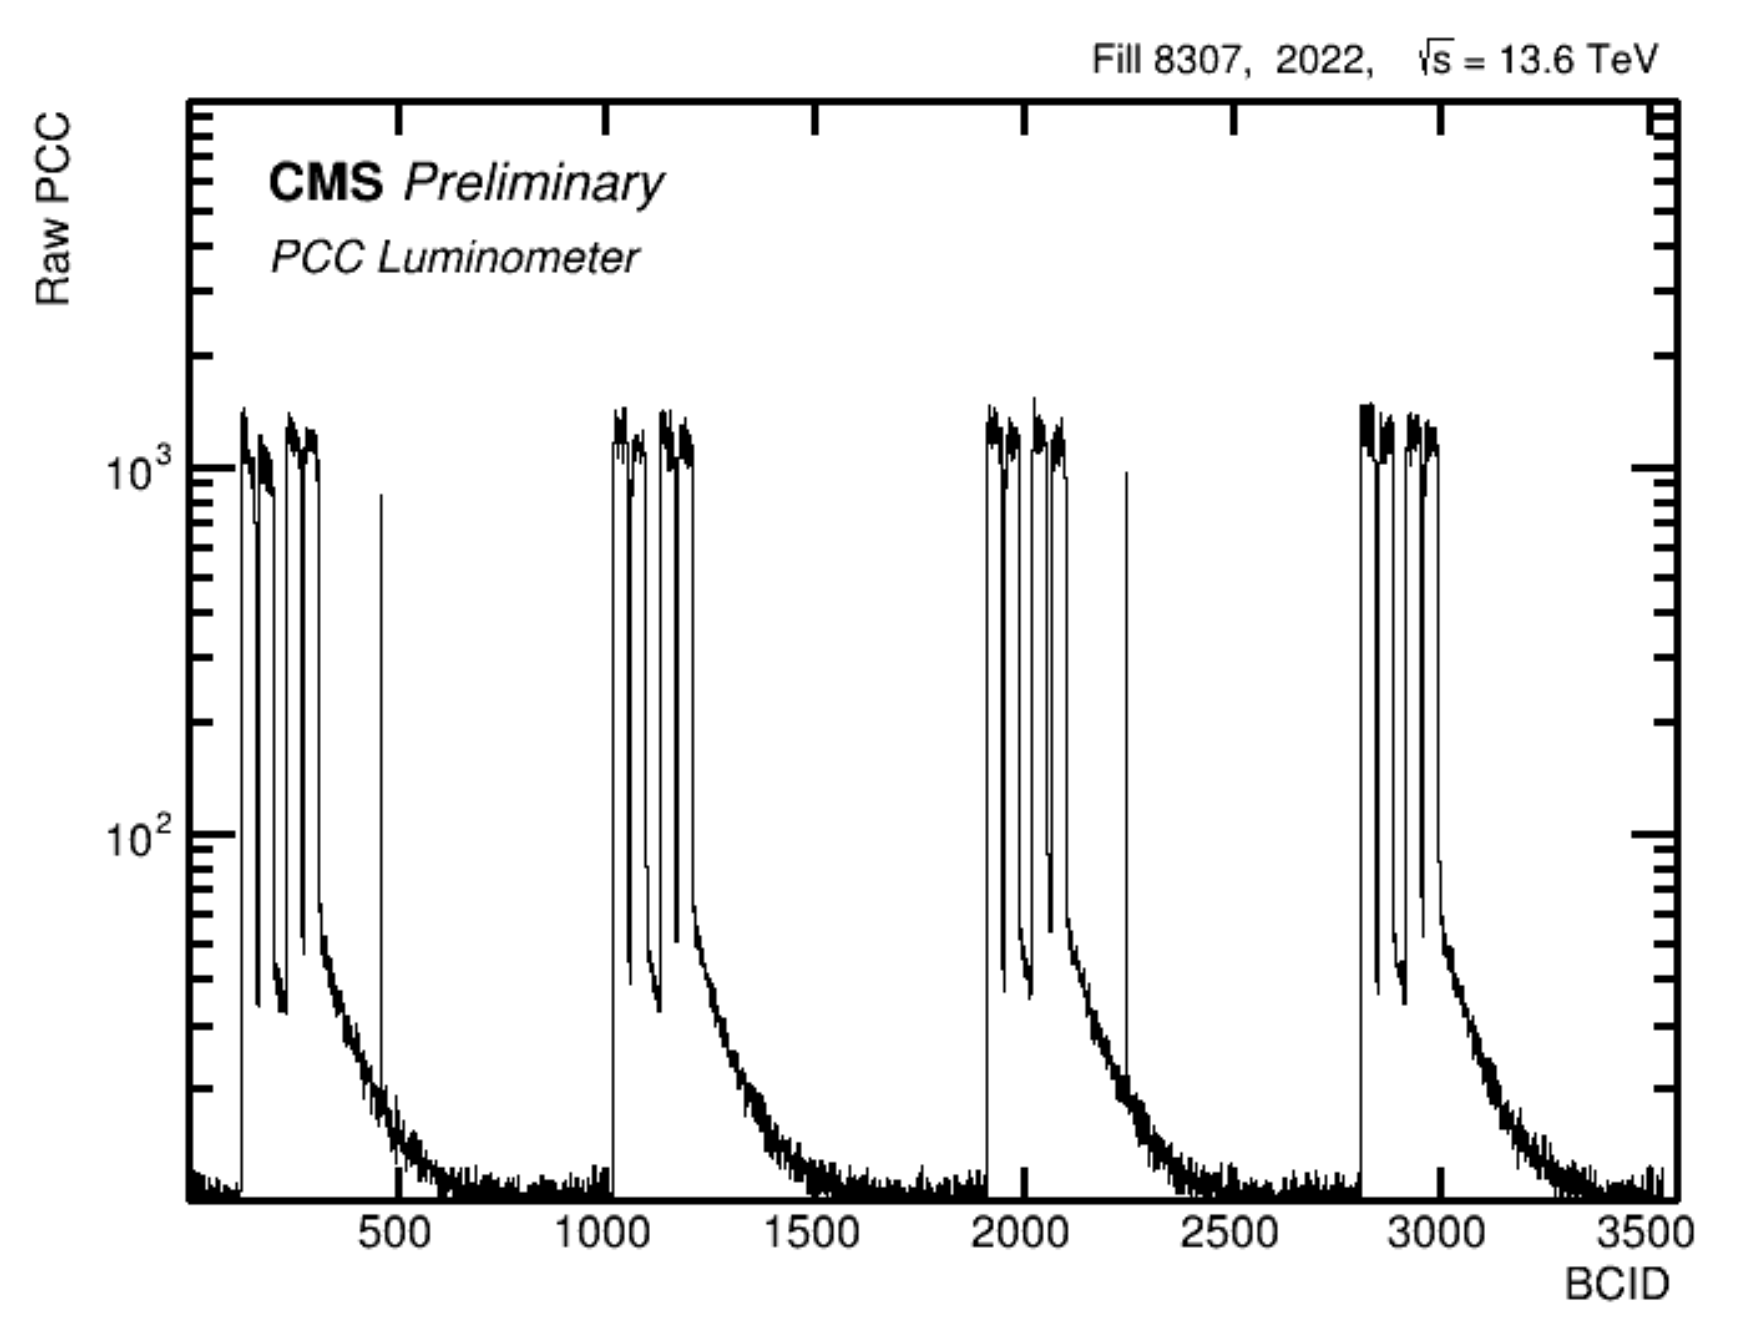
\includegraphics[width=0.8\textwidth]{ashish_thesis/run_361957_ls_block_1.png}
\caption[Raw PCC run 361957]{%                                                                                                                                           
 PCC per bx for fill 8307 for one 50 LS block. The first and ninth train are used to fit the afterglow tail.
}
\label{fig:period_bound_101}
\end{figure}

\begin{figure}[!htp]
\centering
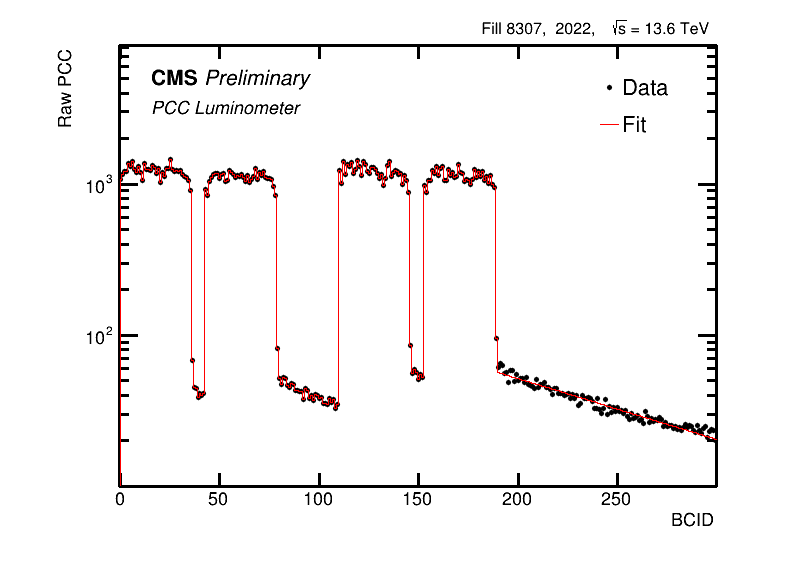
\includegraphics[width=0.8\textwidth]{ashish_thesis/afterglow_fit_2022_1.png}
\caption[Afterglow fit 4-wagon]{%                                                                                                                                                                                                                                                                                      
 Fit to 4-wagon train.
}
\label{fig:period_bound_102}
\end{figure}

%\begin{figure}[!htp]
%\centering
%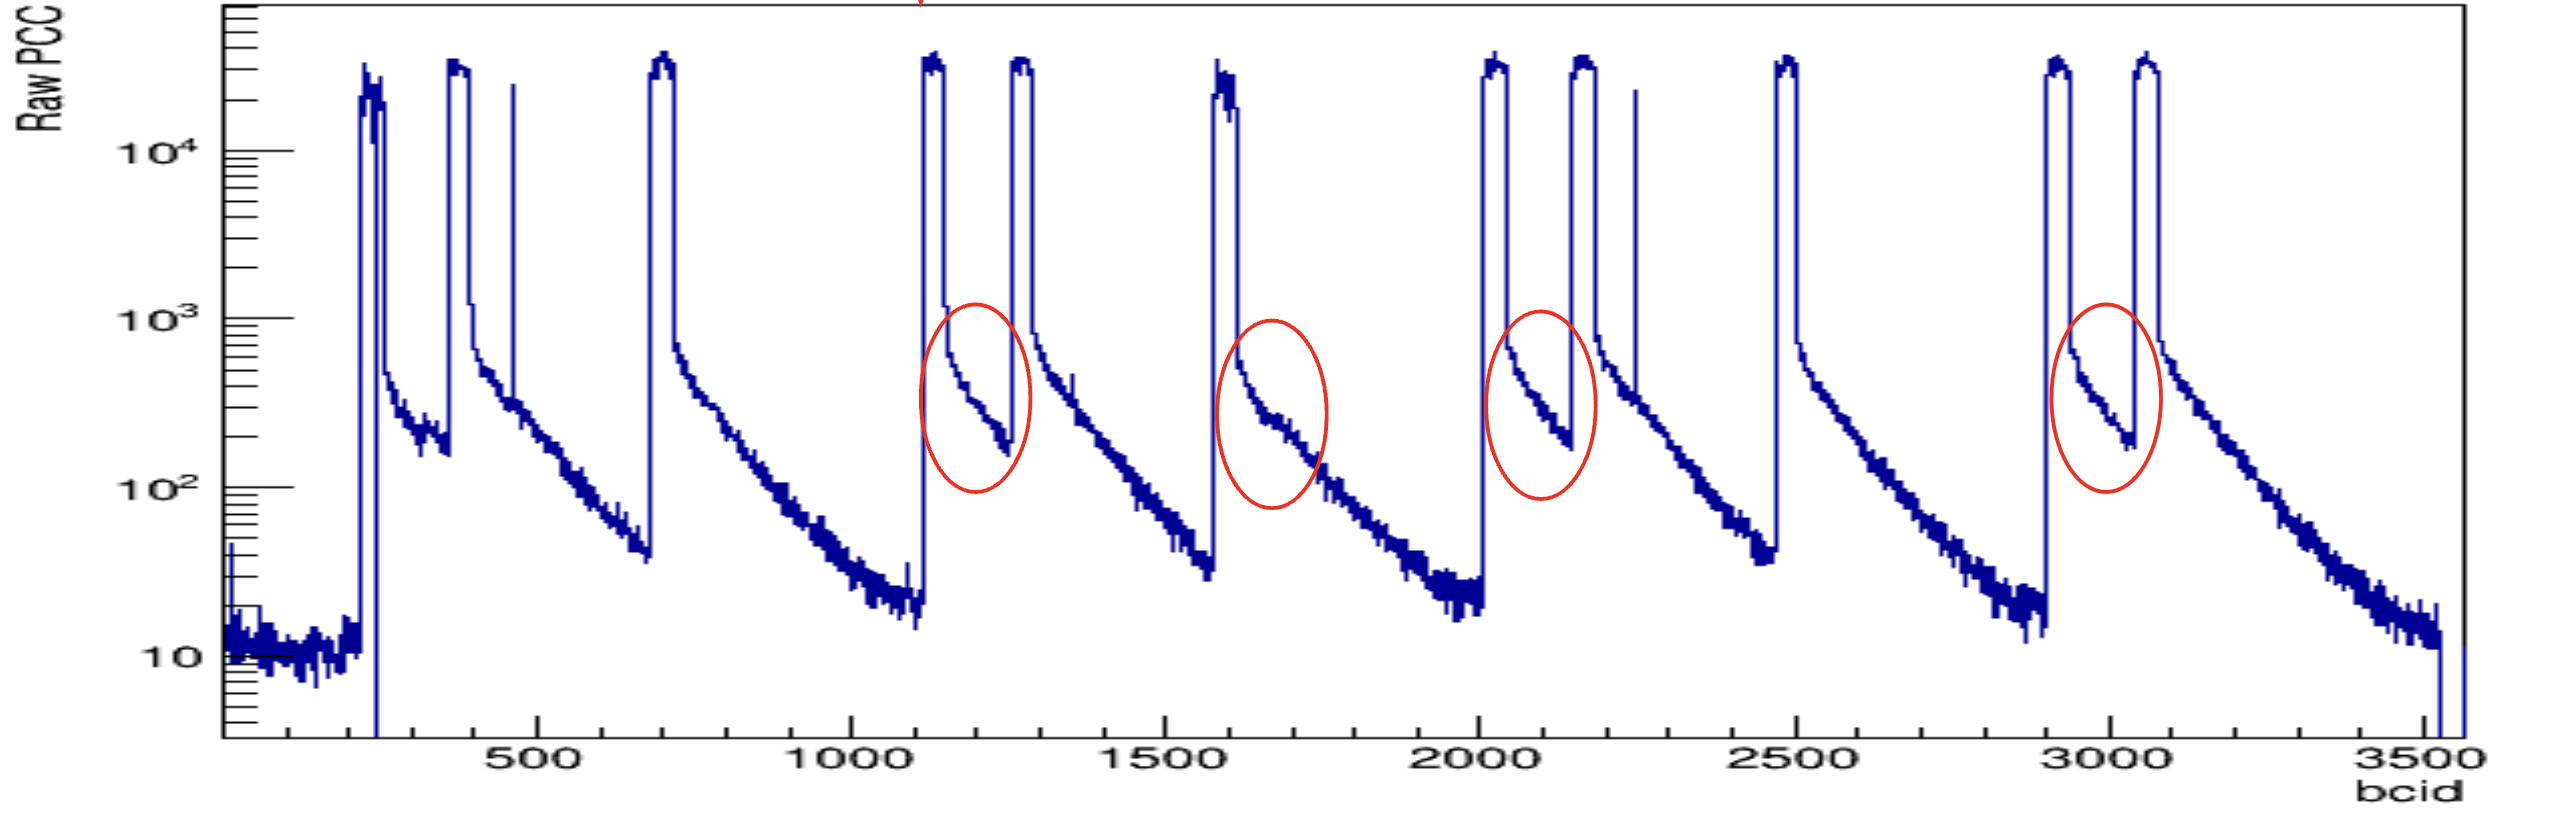
\includegraphics[width=1\textwidth]{ashish_thesis/Run2022_af_model_run.png}
%\caption[Raw PCC run 366800]{%                                                                                                                         
% PCC per bunch crossing for run number 366800. Red circles are the trains that are fit.
%}
%\label{fig:period_bound_101}
%\end{figure}


%\begin{figure}[!htp]
%\centering
%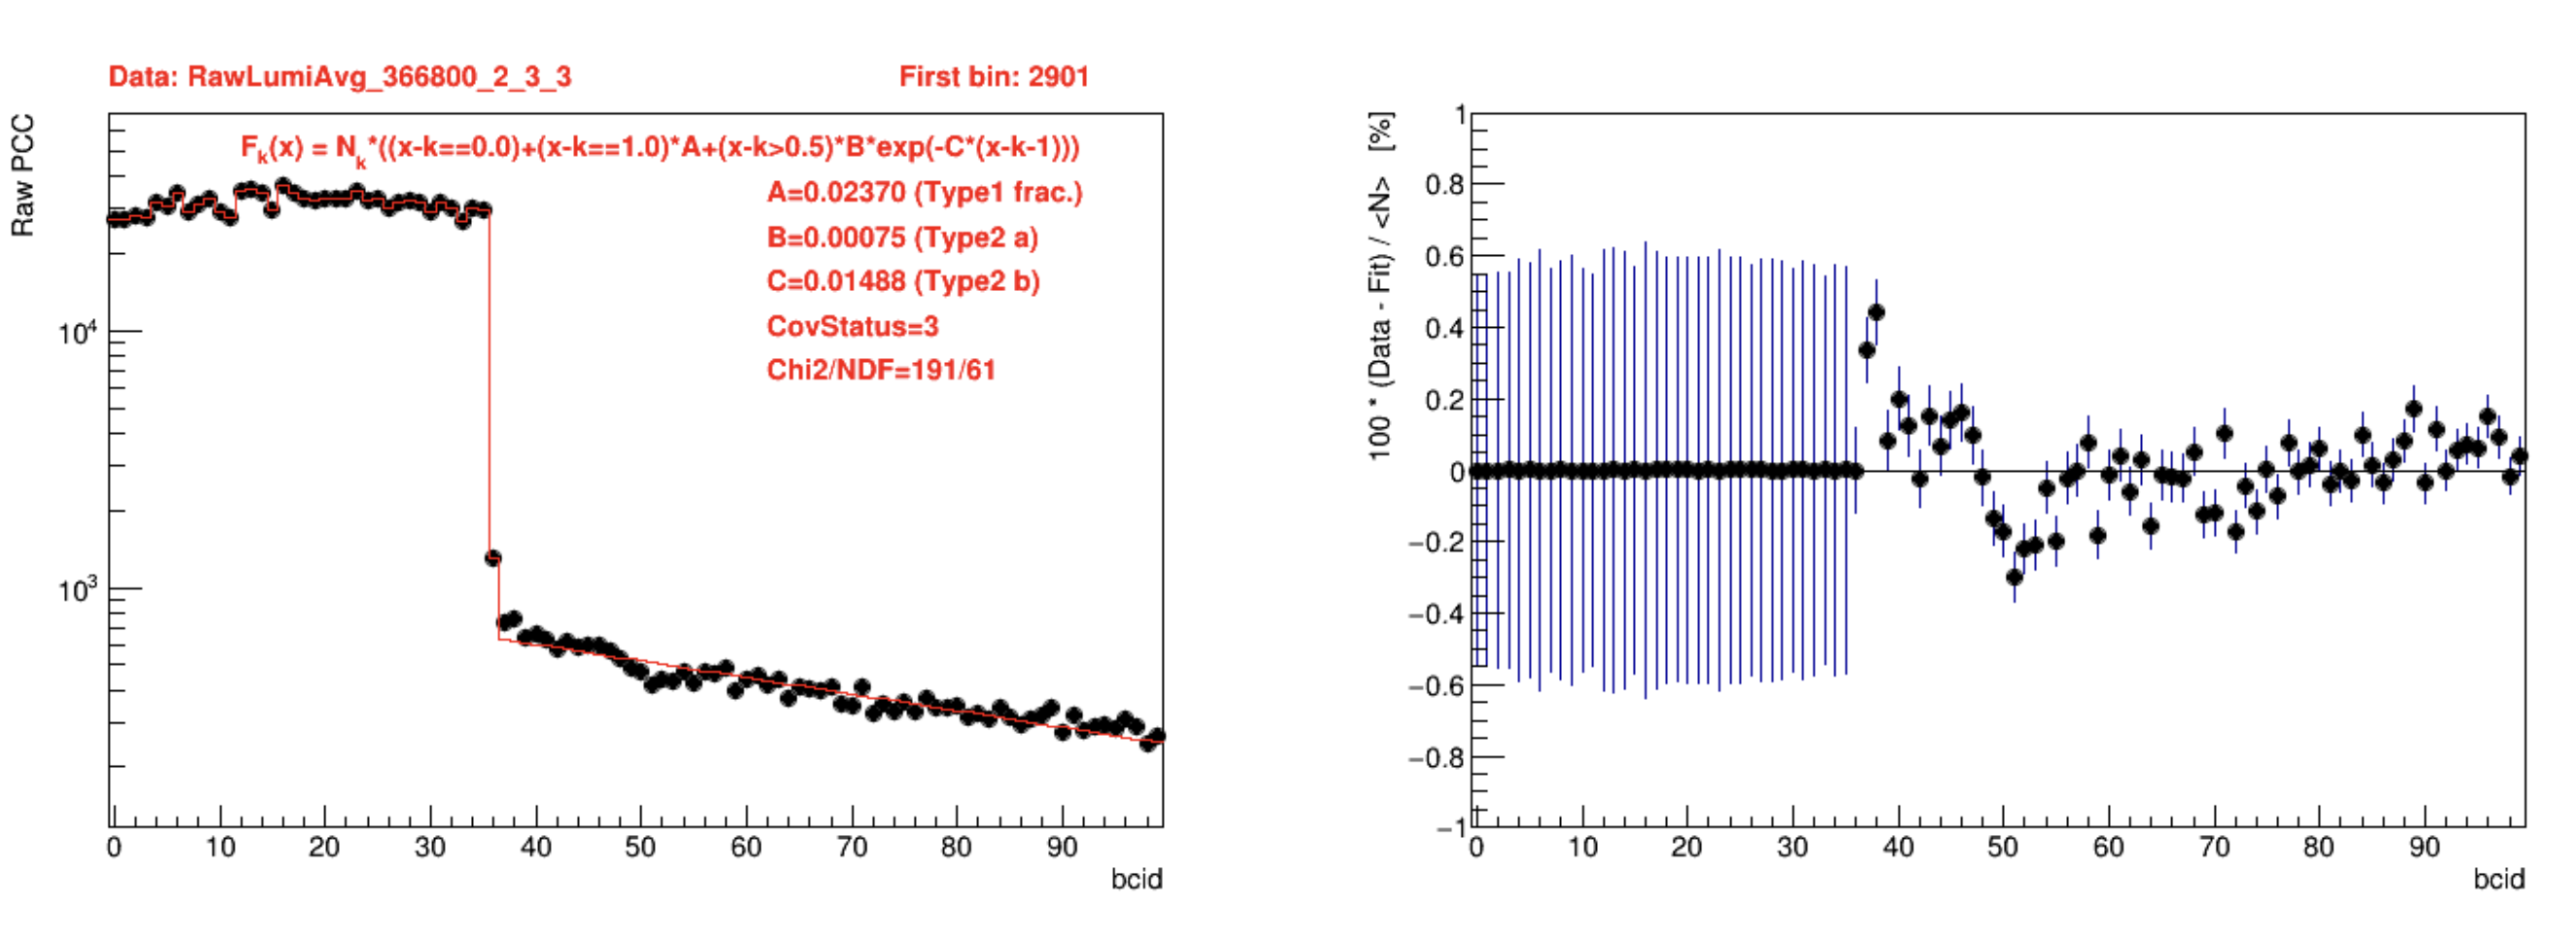
\includegraphics[width=1\textwidth]{ashish_thesis/2022_four_wagon_fit.png}
%\caption[Four wagon fit]{%                                                                                                                         
% Fit for four wagon train using PCC raw data.
%}
%\label{fig:period_bound_102}
%\end{figure}

%\begin{table}[ht]
 % \centering
  %\caption[Type 2 parameters]{Type 2 afterglow parameters for increasing number of trains.}
%\begin{tabular}{cccc}
%\textbf{Train} & \textbf{Type1 f} & \textbf{Type2 a} & \textbf{Type2 b}\\
%\hline
%Train 1 & $1.98 \times 10^{-2} \pm 1.3 \times 10^{-3}$ & $7.58 \times 10^{-4} \pm 1.2 \times 10^{-5}$ & $1.53 \times 10^{-2} \pm 3.6 \times 10^{-4}$\\
%Train 2 & $1.35 \times 10^{-2} \pm 1.7 \times 10^{-3}$ & $8.35 \times 10^{-4} \pm 1.5 \times 10^{-5}$ & $1.46 \times 10^{-2} \pm 4.0 \times 10^{-4}$\\
%Train 3 & $2.25 \times 10^{-2} \pm 1.5 \times 10^{-3}$ & $7.76 \times 10^{-4} \pm 1.2 \times 10^{-5}$ & $1.55 \times 10^{-2} \pm 3.6 \times 10^{-4}$\\
%Train 4 & $2.36 \times 10^{-2} \pm 1.3 \times 10^{-3}$ & $7.53 \times 10^{-4} \pm 1.2 \times 10^{-5}$ & $1.48 \times 10^{-2} \pm 3.6 \times 10^{-4}$\\
%\end{tabular}
%\caption[Type 2 parameters]{Type 2 afterglow parameters for increasing number of trains.}
%\label{table:trains_data}
%\end{table}

\begin{comment}

\begin{figure}[!htp]
\centering
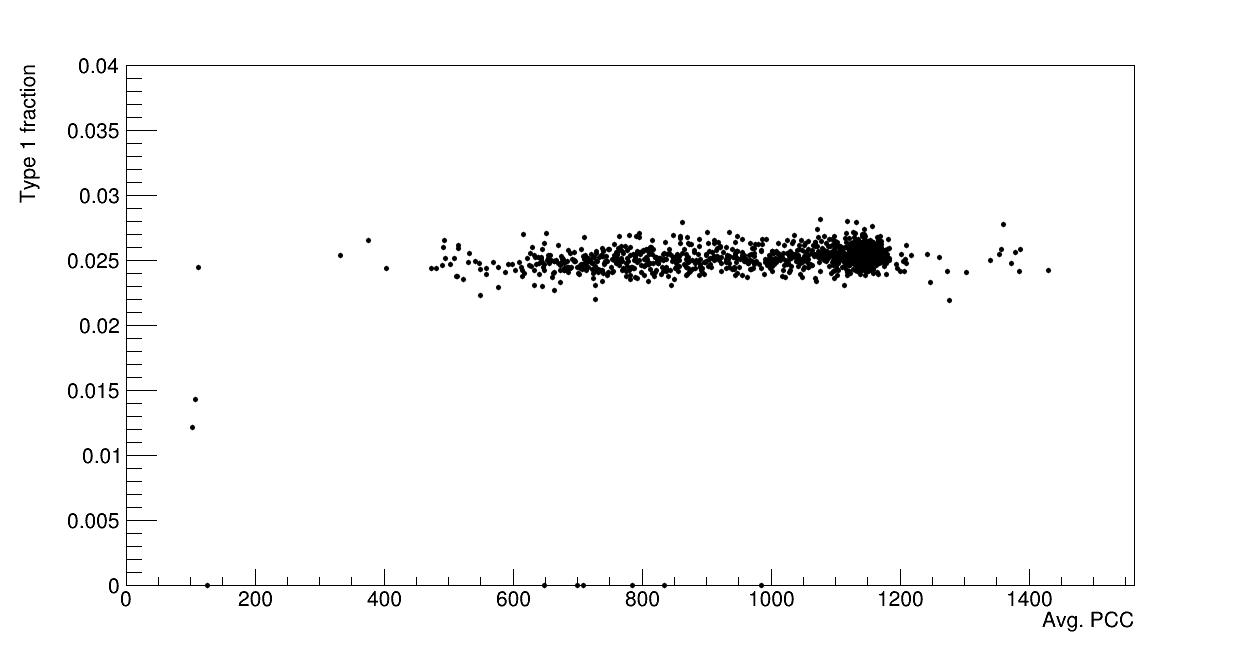
\includegraphics[width=1\textwidth]{ashish_thesis/afterglow_t1f_vsinstlumi.png}
\caption[2022 PCC type 1 afterglow fraction]{%                                                                                                                             
  PCC afterglow correction type 1 fraction as a function of instantaneous luminosity for period Run 2022F. The residual fraction is given by the ratio of the luminosity of the first empty bunch immediately following a colliding bunch to the luminosity of the colliding bunch.

}
\label{fig:period_bound_44}
\end{figure}

\begin{figure}[!htp]
\centering
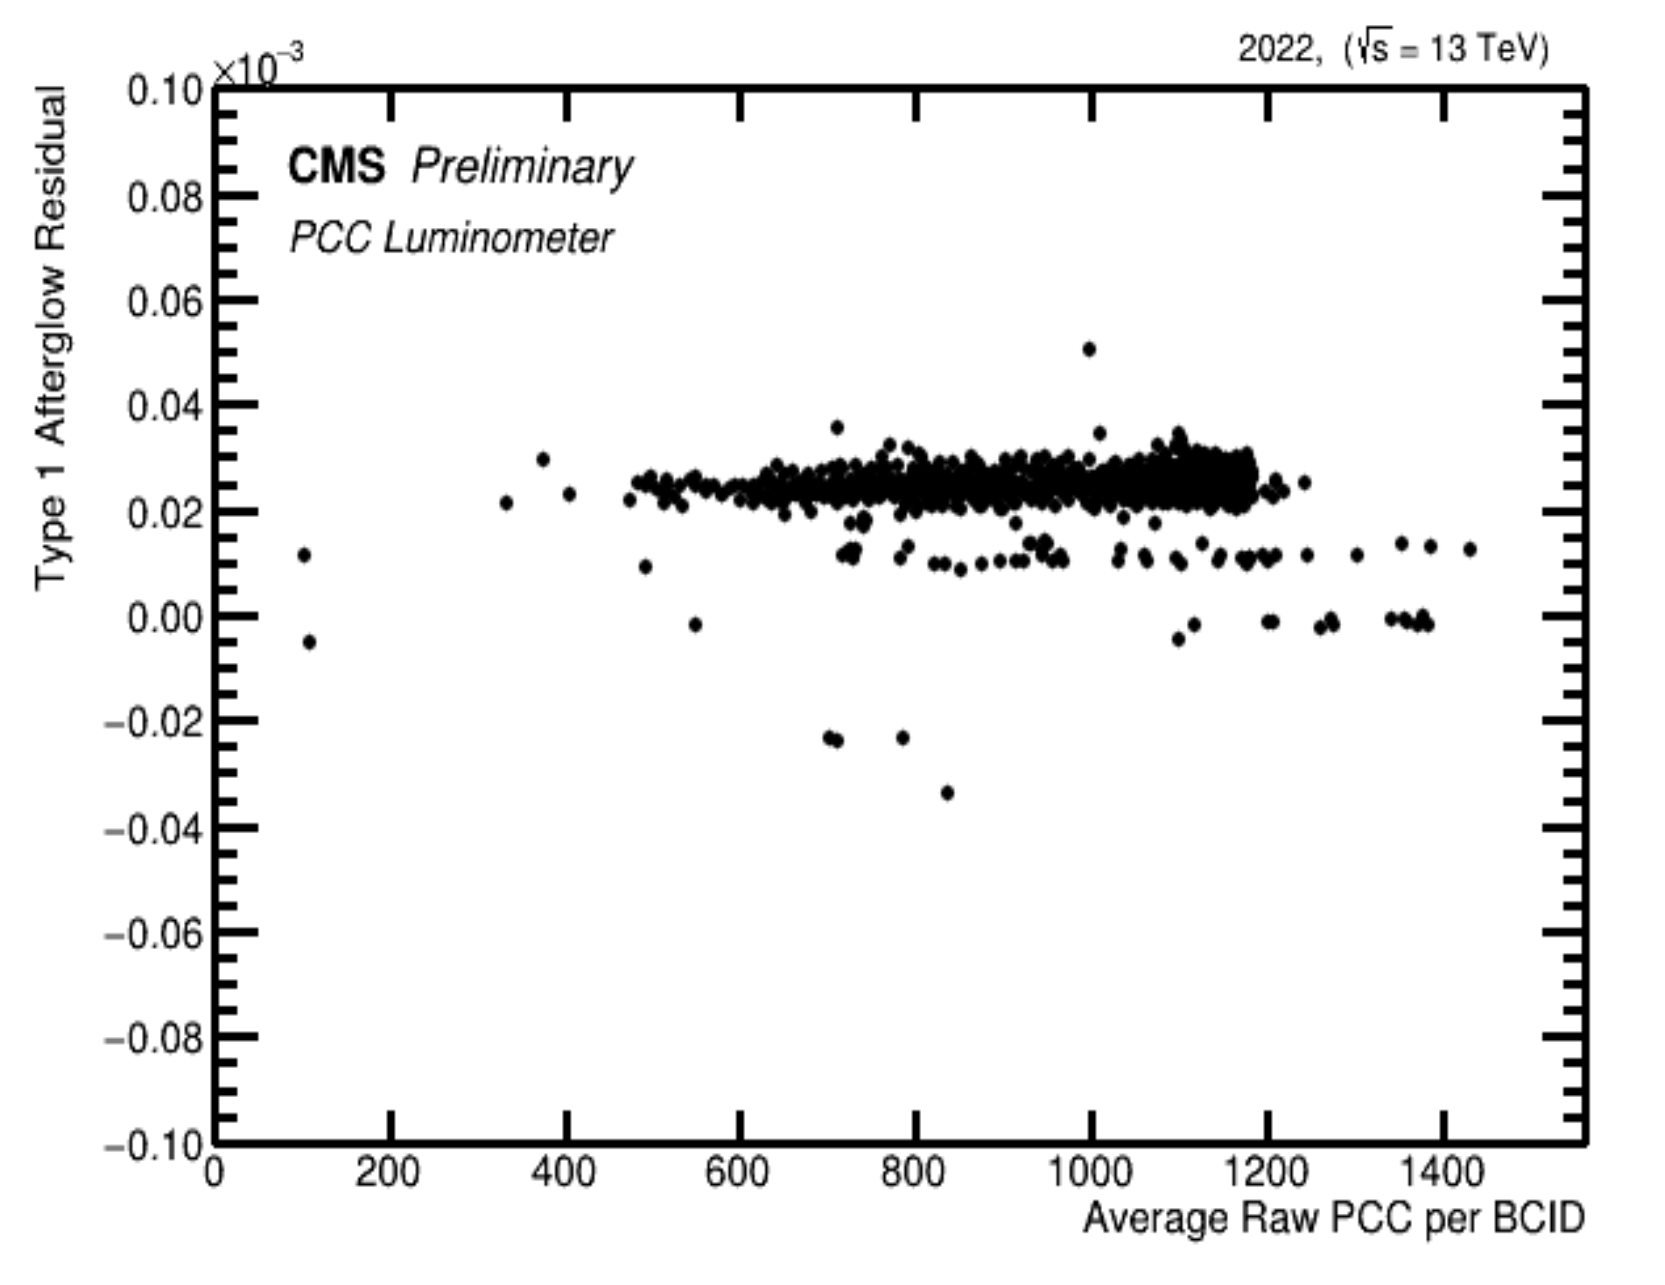
\includegraphics[width=1\textwidth]{ashish_thesis/afterglow_t1res_vsinstlumi.png}
\caption[2022 PCC Type 1 afterglow residuals]{%                                                                                                                                             
 PCC afterglow correction type 1 residual as a function of instantaneous luminosity for period Run 2022F. The residual fraction is given by the ratio of the luminosity of the first empty bunch immediately following a colliding bunch to the luminosity of the colliding bunch.

}
\label{fig:period_bound_44}
\end{figure}



\begin{figure}[!htp]
\centering
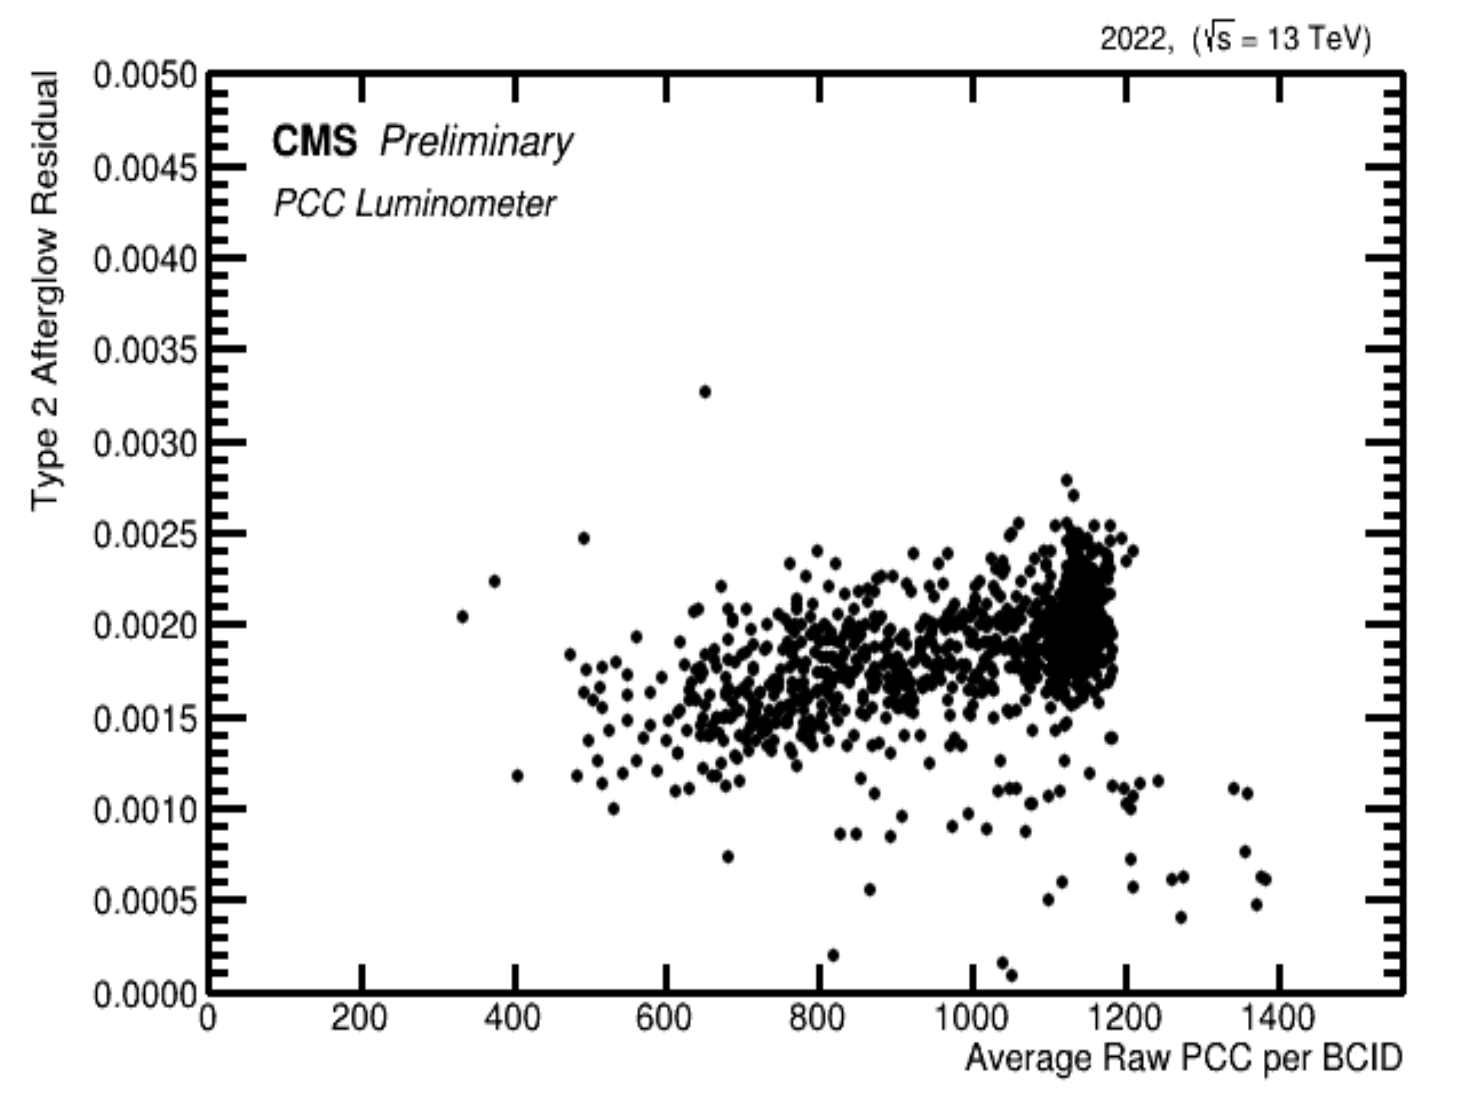
\includegraphics[width=1\textwidth]{ashish_thesis/afterglow_t2res_vsinstlumi.png}
\caption[2022 PCC type 2 afterglow residuals]{%                                                                                                                                             
Type 2 residual as a function of instantaneous luminosity for period 2022F. These are given by the ratio of the luminosity of the second empty bunches after a colliding bunch to the luminosity of the colliding bunch.
}
\label{fig:period_bound_45}
\end{figure}

\end{comment}


\begin{comment}

\begin{figure}[!htp]
\centering
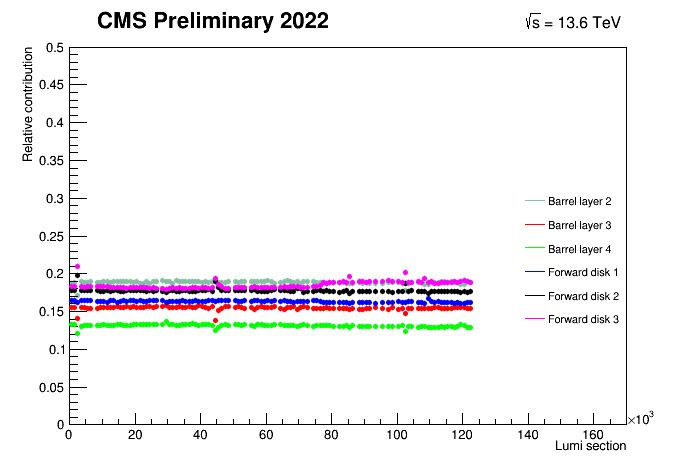
\includegraphics[width=1\textwidth]{ashish_thesis/PCC_stability_2022_L0veto.png}
\caption[Pixel detector stability plots without veto list]{%                                                                                                                                      
  Luminosity fraction of pixel detector for various layer and disks as a function of lumi section for Layer 1 module veto. 
}
\label{fig:period_bound}
\end{figure}

\begin{figure}[!htp]
\centering
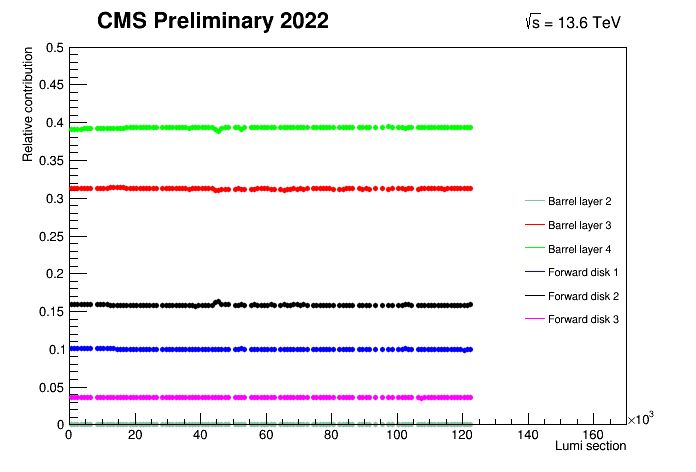
\includegraphics[width=1\textwidth]{ashish_thesis/2022_pcc_stability.png}
\caption[Pixel detector stability plots with veto list]{%                                                                                                                                              
  Stability profiles of pixel detector layer and disk modules for 4\% rms common module veto list.
}
\label{fig:period_bound}
\end{figure}


\begin{figure}[h]
  \centering
  \begin{subfigure}[b]{0.8\textwidth}
    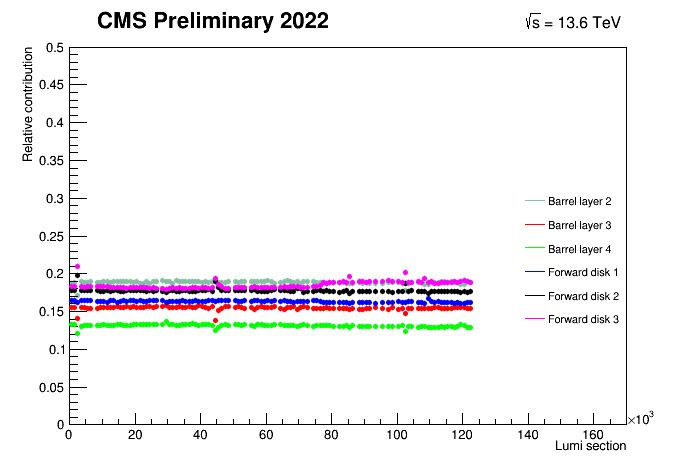
\includegraphics[width=\textwidth]{ashish_thesis/PCC_stability_2022_L0veto.png}
    %\caption{Image 1}                                                                                                                                                                     
  \end{subfigure}
  %\hfill % or \hspace{5mm} for a specific horizontal space                                                                                                                                 
  %\begin{subfigure}[b]{0.49\textwidth}
   % 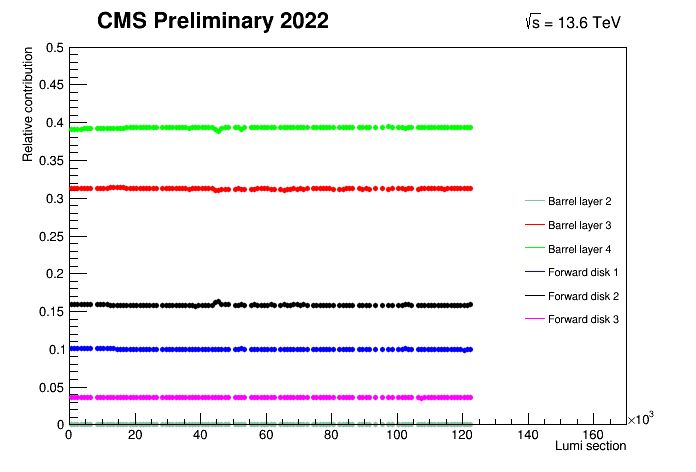
\includegraphics[width=\textwidth]{ashish_thesis/2022_pcc_stability.png}
    %\caption{Image 2}                                                                                                                                                                     
  %\end{subfigure}
  \caption[Pixel detector stability plots without and with common veto list]{Luminosity fraction of pixel detector for various layer and disks as a function of lumi section for Layer 1 module veto.} %Right: Stability profiles of pixel detector layer and disk modules for 4\% rms common module veto list.}
  \label{fig:stabprof}
\end{figure}

\end{comment}

\newpage
Background estimations are obtained from the Random trigger datasets, processed in 50 LS blocks. The corrections, determined from these backgrounds, are subsequently applied to the zero-bias data. %Post-fitting residuals help in verifying the accuracy of the process.
While Type 1 residuals are minimal, Type 2 shows a slight deviation of around 0.2\% as shown in Fig. \ref{fig:period_bound_45}.

Comparable patterns are observed for 2022 periods E, F and G. During periods C and D, data was limited to the "AlCALumiPixelsEXPRESS" stream with an outdated module selection. Consequently, direct re-evaluation became unfeasible. As a solution, stored afterglow corrections evaluated in the CMS prompt calibration stage, corrected by a factor 1.008 from period E data, were applied.


\begin{figure}[H]
\centering
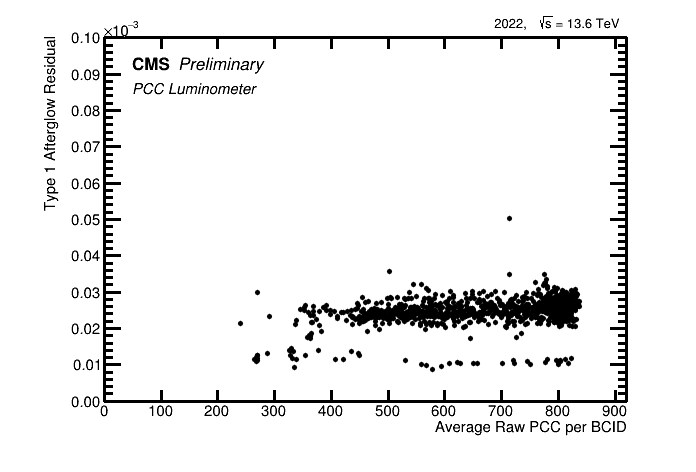
\includegraphics[width=0.9\textwidth]{ashish_thesis/afterglow_t1res_vsinstlumi_1.png}
\caption[2022 PCC type 1 afterglow residuals]{%                                                                                                                                                                             
 PCC afterglow correction type 1 residual as a function of instantaneous luminosity for period Run 2022F. The residual fraction is given by the ratio of the luminosity of the first empty bunch immediately following a colliding bunch to the luminosity of the colliding bunch.

}
\label{fig:period_bound_44}
\end{figure}


\begin{figure}[H]
\centering
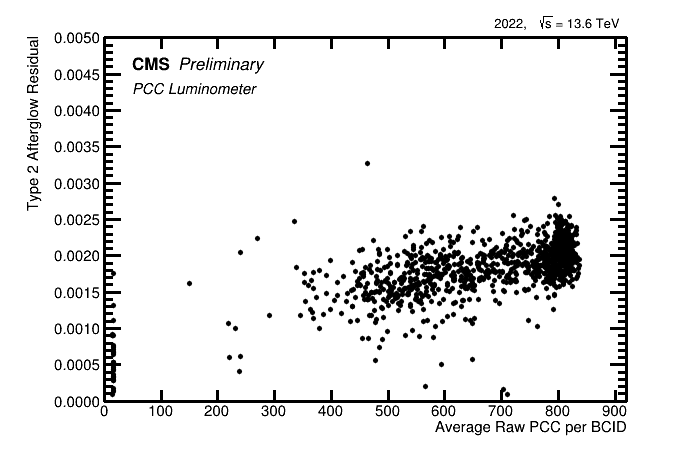
\includegraphics[width=0.9\textwidth]{ashish_thesis/afterglow_t2res_vsinstlumi_1.png}
\caption[2022 PCC type 2 afterglow residuals]{%
  Type 2 residual as a function of instantaneous luminosity for period 2022F. These are given by the ratio of the luminosity of the second and following empty bunches after a colliding bunch to the luminosity of the colliding bunch.
}
\label{fig:period_bound_45}
\end{figure}

\section{PCC instantaneous and integrated luminosity}

PCC instantaneous luminosity provides a measure of the collider performance and is graphically represented in Fig. \ref{fig:period_bound_1000045}. Each fill in the graph consistently displays a sequence of characteristics related to luminosity. The process initiates with ramp-up periods, where a swift increase in luminosity is evident. This surge is subsequently followed by leveling parts, where luminosity stabilizes and plateaus. As the fill progresses, burn-off parts emerge, marked by a gradual decline in luminosity. Interspersed within the graph are notable, sharp drops to lower luminosity levels, characteristic of emittance scans. As each fill reaches its culmination, pronounced drops are observable, signifying the end of fill events. This cyclical pattern is evident across all fills, underscoring the systematic nature of the process. Integrated luminosity accumulates this data over time \cite{pas_22}. %For 2022, the total PCC integrated luminosity is calculated to be 38.61 $fb^{-1}$ \cite{pas_22}. %\cite{bril2023randomzerobias}. 

\begin{figure}[H]
\centering
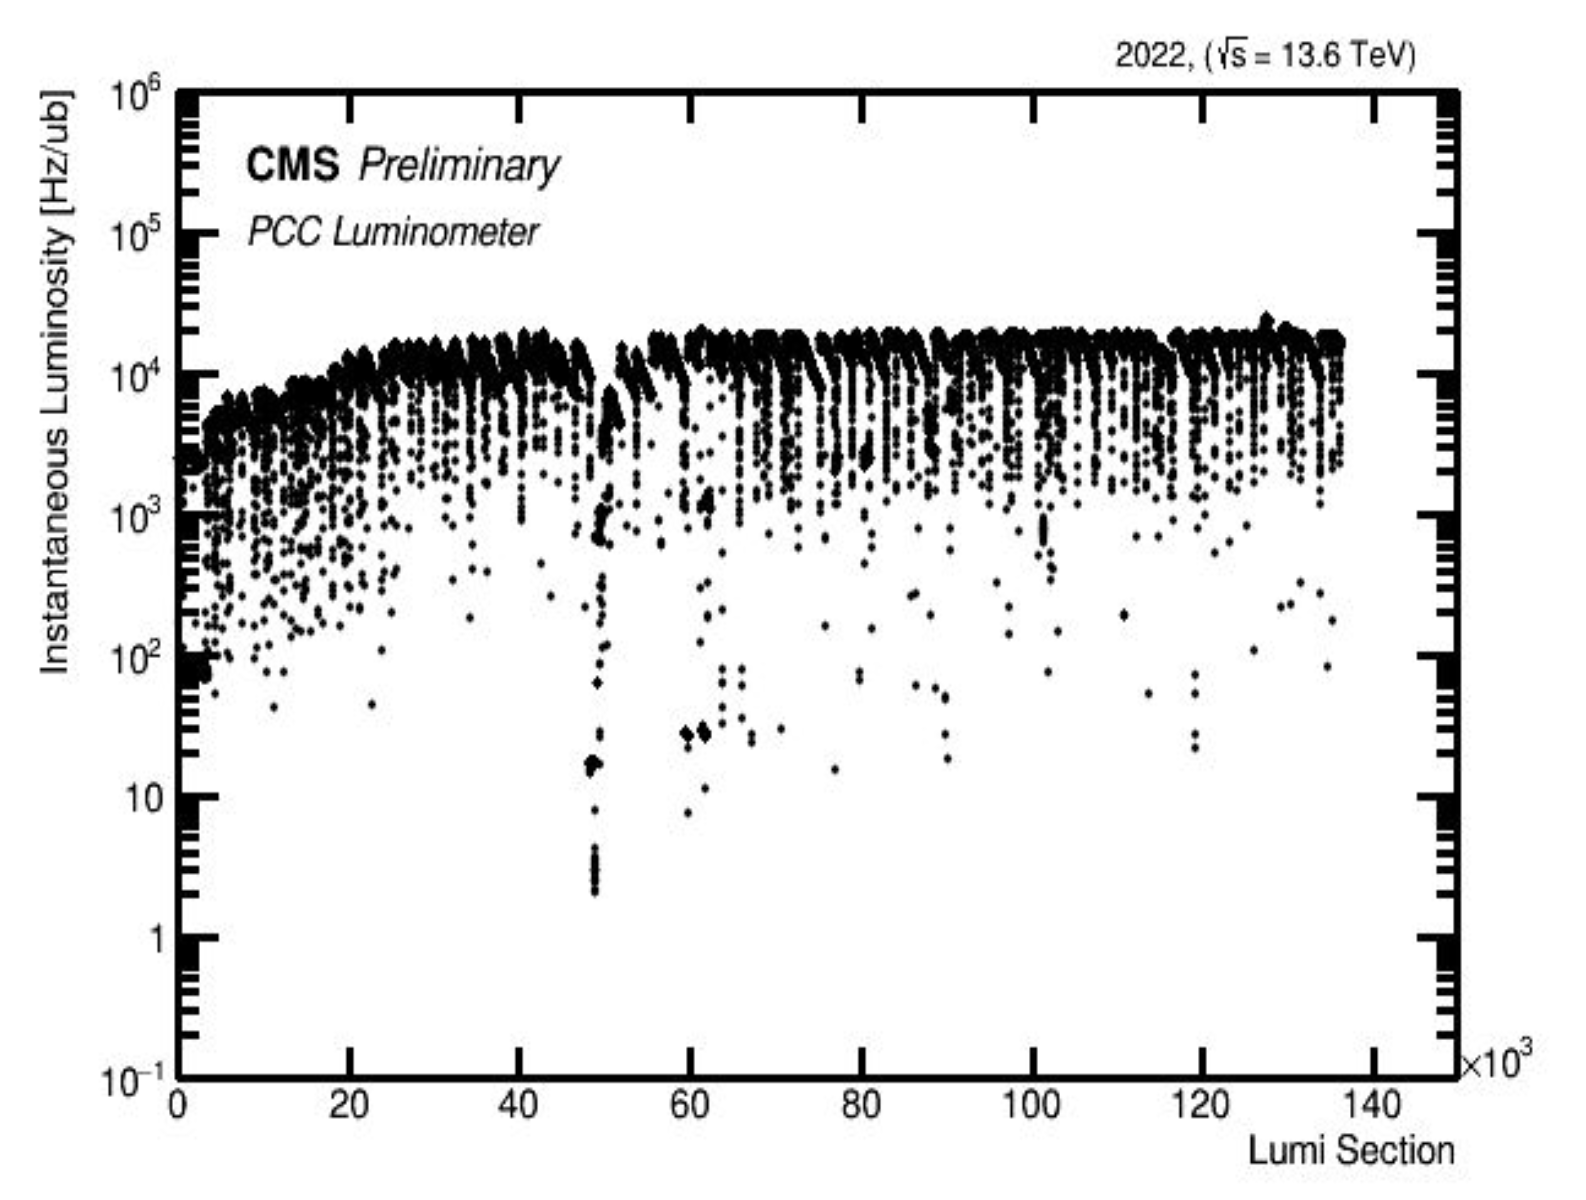
\includegraphics[width=0.9\textwidth]{ashish_thesis/PCClumivslumisection_2022.png}
\caption[2022 PCC inst. luminosity]{%
  PCC instantaneous luminosity as a function of lumi section for entire 2022 year.
  
}
\label{fig:period_bound_1000045}
\end{figure}


\section{Systematic uncertainties}

Various sources of systematic uncertainty come into play, affecting the precision of the results. These uncertainties arise from factors such as detector calibrations, alignment, temporal drifts in the detector response, modeling of the beam conditions, and potential nonlinearities in the detector response. Each of these factors necessitates careful calibration, modeling, and validation processes to ensure the highest accuracy in the luminosity measurement. %Addressing these systematic uncertainties is pivotal for the CMS collaboration to draw meaningful and reliable conclusions from its data.

\subsection{vdM calibration uncertainties}

\begin{itemize}

\item XY-factorization: In the vdM calibration, the luminous area estimation, based on beam shapes, can lead to the "factorization bias." Methods to study factorization bias are 

\begin{itemize}

\item \textbf{Beam-Imaging Method:} By using reconstructed collision vertices, this method estimates actual beam densities, which helps in refining the vdM-based luminous area. The following equation describes the relationship between the number of interaction points (vertices) and the proton densities of two beams at specific positions.

\begin{equation}
N_{\text{vertices}}(x, y; \Delta x) \propto \rho_1(x + \Delta x, y) \cdot \rho_2(x, y) \bigotimes V
\end{equation}

where
\begin{itemize}
  \item \(N_{\text{vertices}}(x, y; \Delta x)\): Represents the number of vertices or interaction points at a given beam separation in the x and y directions. The term \(\Delta x\) indicates the change or step in the x-direction.
  
  \item \(\rho_1(x + \Delta x, y)\) and \(\rho_2(x, y)\): Represent the proton density distributions of the two beams at specific positions. The densities indicate how many protons are present at a particular point in space.
  
  \item \(\bigotimes V\): Represents a convolution operation with \(V\), the vertex resolution. It's a mathematical way to combine two functions to produce a third function, used here to account for the limitations in measuring the exact position of the vertices due to the resolution of the detectors.
\end{itemize}

Combining all steps, we get

\begin{align}
\sum_{\Delta x} N_{\text{vertices}}(x, y; \Delta x) &\propto \sum_{\Delta x} \left[ \rho_1(x + \Delta x, y) \cdot \rho_2(x, y) \right] \otimes V \nonumber \\
&\approx \int_{\Delta x} \left[ \rho_1(x + \Delta x, y) \cdot \rho_2(x, y) \right] \otimes V d\Delta x
\end{align}

The number of interaction points (vertices) observed depends on the proton densities of the two beams at specific positions, the separation between the beams in the x and y directions, and the precision with which these interaction points can be measured. By studying the change in the number of interaction points as the beams are moved closer or further apart, we can know about the proton densities of the beams and their distribution in space. The convolution with \(V\) ensures that the measurements are adjusted for the limitations of the detectors.

%Data from four LHC scans are compiled into histograms and fitted using models describing beam shapes. Three fit models are employed: single-Gaussian (SG), double-Gaussian (DG), and super-Gaussian (SupG), each defining the beam shape differently based on beam widths and correlation parameters. The DG and SupG models involve combinations of "narrow" and "wide" components with specific parameter restrictions. The super-Gaussian fit most accurately describes the beam-imaging scan data, showing consistent results across all BCIDs.

\item \textbf{Diagonal Scans:} Moving the beams at a 45° angle to the standard vdM direction in diagonal scans captures data across both x and y dimensions at the same time. This approach provides a unique view of how protons overlap and distribute in a two-dimensional plane. Instead of just seeing a linear view from one direction, the diagonal movement offers a comprehensive picture of the spread and patterns of protons in 2D.

\item \textbf{Offset Scans:} In offset scans, the added separation in the direction not being actively scanned gives additional data points that wouldn't be captured in a standard vdM scan. This added separation means that the scan captures proton densities at slightly shifted positions. When combined with the regular vdM scan data, it offers a more detailed view of the proton distribution in two dimensions, helping to understand variations and potential irregularities in the 2D proton density.

  %\item \textbf{Diagonal and Offset scans:} In diagonal scans, beams are moved simultaneously in x and y, at a 45° angle to the standard vdM direction offering a different perspective of overlap. In offset scans, along with the regular vdM scan movement, there's an added separation in the direction not being actively scanned. Luminometers like BCM1F, BCM1FUTCA, PLT were analyzed.
   % Background, orbit drift, beam-beam corrections are applied. An extra orbit drift correction came from rate matching and 1D vdM fits. Data is saved as 2D graphs while VdMFramework uses less precise 1D graphs. 2D fit functions include Single Gaussian, Super Gaussian, q-Gaussian, and variations of Double Gaussian. 2D fitting involved pairing on-axis and off-axis scans. Off-axis scans were matched to the nearest vdM scans, combining rate values for clearer 2D shapes.

%BCID dependence patterns correlate with LHC experiment collisions as there is periodic structure every fourth bunch, influenced by PS Booster effects. Averaged correction across off-axis+on-axis scan pairs is \(0.98 \pm 0.35\).  Detectors' predictions align well. Data encoding reflects types and directions of shifts. Some evidence of an ellipsoidal shape tilted relative to the XY frame. Including all models modifies correction and RMS significantly. Largest contributors to corrections are BCID, model dependence, and OD systematics, yielding a combined RMS of \(0.35\%\). Considering all model uncertainties, this increases to \(0.45\%\).

\end{itemize}

%Factorization bias in VdM calibration is due to the assumption of factorizable beam shapes. This can be addressed by reconstructing transverse proton densities during a VdM fill, enabling a comparison of the luminous area to expected outcomes. The beam-imaging method, applied by CMS, uses reconstructed vertices to extract proton densities. Other methods, like diagonal and offset scans, examine different luminous area sections to understand factorization biases. CMS has explored these methods, with recent studies ongoing from 2022 data.

\item Bunch to bunch uncertainty: The "bunch to bunch variation of PCC visible cross section" refer to how much the measured visible cross-section (and thus, the measured luminosity) changes from one bunch crossing to another as shown in Table \ref{tab:my_labeltt}. Variations could arise from different factors such as varying numbers of protons per bunch, spatial distribution of protons within the bunches, and the specific conditions of the pixel detector at the time of each bunch crossing. %These variations are important to monitor as they can impact the precision of the luminosity measurement, which in turn affects the accuracy of the results obtained from the physics analyses conducted with the data.
If significant variations are observed, it may be necessary to adjust the analysis to account for these differences. 

%\begin{figure}[!htp]
%\centering
%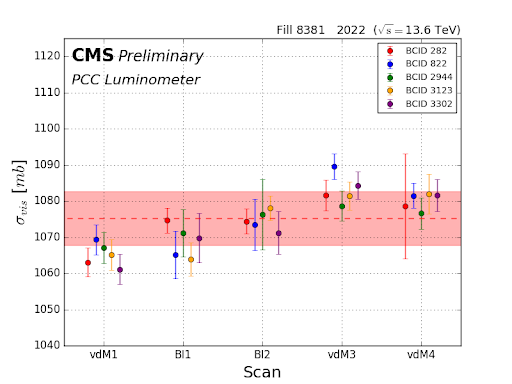
\includegraphics[width=0.8\textwidth]{ashish_thesis/2022_sigma_vis_btob_variation.png}
%\caption[$\sigma_{vis}$ Bunch Variation]{%                                                                                                                                             
 % Bunch to bunch variation of PCC visible cross section where the red line is the average value. Red band depicts the $\pm$ one RMS of the values.
%}
%\label{fig:period_bound_99}
%\end{figure}

%\begin{table}[!htp]
 % \centering
  %\caption[$\sigma_{vis}$ bunch uncertainty]{Bunch to bunch variation of visible cross section. $N_b$ is the number of bunches in the vdM scan.}
%\begin{tabular}{ccccc}
 %& \textbf{Scan} & \textbf{$\sigma_{vis}$ [mb]} & \textbf{RMS [mb]} & $\frac{\frac{\textbf{RMS}}{\sqrt{N_b}}}{\sigma_{\textbf{vis}}}$  [\%]} \\
%\hline
%1 & vdM1 & 4147.71 & 12.56 & 0.13 \\
%2 & Img1 & 4151.50 & 12.22 & 0.13 \\
%3 & Img2 & 4146.04 & 5.39 & 0.05 \\
%4 & vdM3 & 4174.31 & 9.18 & 0.10 \\
%5 & vdM4 & 4145.64 & 6.96 & 0.08 \\
%\end{tabular}
%\label{tab:my_label}
%\end{table}

\begin{table}[!htp]
  \centering
  \caption[Bunch uncertainty]{Bunch to bunch variation of visible cross section (as shown in Fig. \ref{fig:period_bound_99}). $N_b$ is the number of bunches in the vdM scan. SEM is the standard error on the mean.}
\begin{tabular}{cccc}
\textbf{Scan} & \textbf{$\sigma_{vis}$ [mb]} & \textbf{RMS [mb]} & (SEM/$\sigma_{vis}$) [\%] \\
\hline
vdM1 & 1065.09 & 2.89 & 0.1286 \\
Img1 & 1070.14 & 3.94 & 0.1746 \\
Img2 & 1075.38 & 2.35 & 0.1040 \\
vdM3 & 1083.58 & 3.70 & 0.1616 \\
vdM4 & 1080.37 & 2.09 & 0.0920 \\
\end{tabular}
\label{tab:my_labeltt}
%\caption{Bunch to bunch variation of visible cross section. $N_b$ is the number of bunches in the vdM scan.}
\end{table}

%$\frac{\frac{\textbf{RMS}}{\sqrt{N_b}}}{\sigma_{\textbf{vis}}}$

\newpage
\item Scan to scan uncertainty: PCC visible cross section can exhibit change from one scan to the next. These variations could be due to slight changes in the experimental conditions. The results for each scan are plotted after averaging over five BCIDs as shown in Fig. \ref{fig:period_bound_105}. Each point on this graph represent the result from one scan. A red line is drawn to indicate the average value of the visible cross-section over all the scans. This average value provides a useful comparison point to evaluate the consistency of the individual scan results and identify any potential anomalies or systematic errors.

%\begin{figure}[!htp]
%\centering
%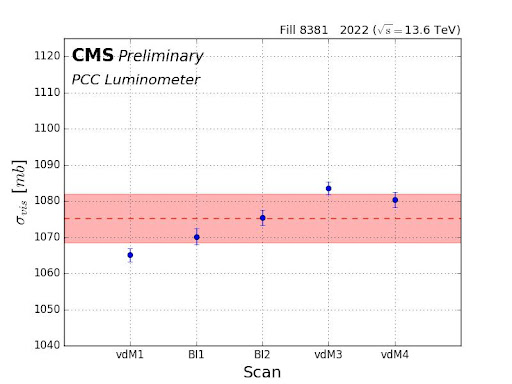
\includegraphics[width=0.6\textwidth]{ashish_thesis/2022_sigma_vis_per_scan.png}
%\caption[2022 PCC visible cross section]{%                                                                                              
 % Visible cross section per scan where red line shows the average value.
%}
%\label{fig:period_bound_105}
%\end{figure}

%Sigma Vis =  4.1694 +- 0.002 (stat) Barns
%0.06\% statistical error
%\section{Systematic uncertainties}

\item Background subtraction: %The process of PCC correction involves eliminating undesired signals from a detector system that are not relevant to the physical phenomenon under study, such as noise or cosmic rays.
  Machine-induced backgrounds are studied using two super separation scans 1 and 2. A floating constant is used in each fit and the uncertainty due to the background level is directly propagated to the result in the visible cross section values.

\begin{comment}
  The results from these scans show significant interpolation, leading to using floating background parameter in the fit which is a constant term to mimic machine induced backgrounds. Any uncertainty in the background rate directly contributes to the uncertainty in the final, corrected rate and thus luminosity. 

\begin{figure}[!htp]
\centering
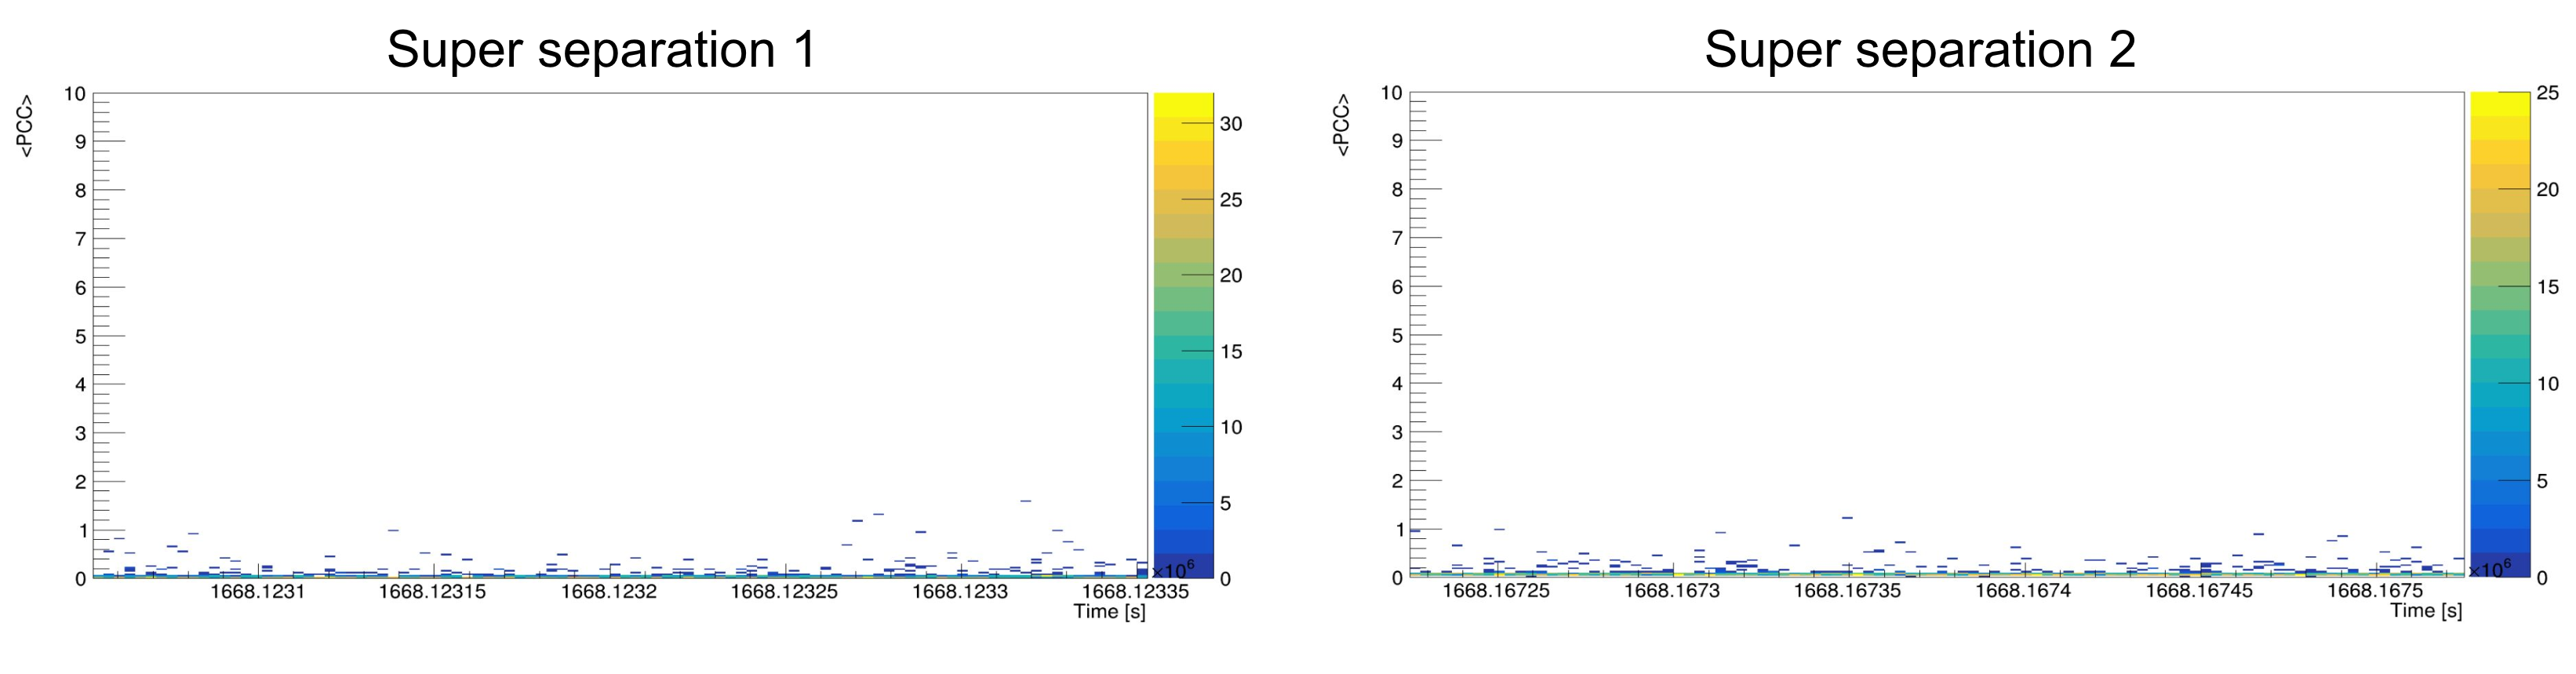
\includegraphics[width=1\textwidth]{ashish_thesis/SS_bkg_2022.png}
\caption[2022 backgound estimation]{%                                                                                                                                              
  2D histogram filled with the Avg. PCC evaluated per NB4, during the Super-Separation window.
}
\label{fig:ssbkg_2022}
\end{figure}

%\begin{comment}

\begin{table}[!htp]
  \centering
  \caption[2022 PCC background rate]{PCC background rate for five BCIDs during super separation scans 1 and 2. Average PCC background rate is calculated by averaging over all five BCIDs.}
    \begin{minipage}{0.45\textwidth}
        \centering
        \begin{tabular}{ccc}
          \hline
            \multicolumn{3}{|c|}{SS 1} \\
            \hline
            BCID & Mean & SEM \\
            \hline
            282 & 0.03917 & 0.00147 \\
            822 & 0.03896 & 0.00130 \\
            2944 & 0.03979 & 0.00145 \\
            3123 & 0.03788 & 0.00132 \\
            3302 & 0.03931 & 0.00130 \\
        \end{tabular}
        \subcaption{SS1_{avg}= 0.039022 +- 0.000613}
    \end{minipage}%
    \hfill
    \begin{minipage}{0.45\textwidth}
        \centering
        \begin{tabular}{ccc}
            \hline
            \multicolumn{3}{|c|}{SS 2} \\
            \hline
            BCID & Mean & SEM \\
            \hline
            282 & 0.07682 & 0.00128 \\
            822 & 0.077513 & 0.00137 \\
            2944 & 0.082114 & 0.00178 \\
            3123 & 0.075385 & 0.00127 \\
            3302 & 0.077605 & 0.00139 \\
        \end{tabular}
        \subcaption{SS2_{avg}= 0.0779018 -+ 0.00060436}
    \end{minipage}
    %\caption{PCC background rate for five BCIDs during super separation scans 1 and 2. Average PCC background rate is calculated by averaging over all five BCIDs.}
    \label{table:side_by_side}
\end{table}


%\begin{comment}

\begin{table}[h]
    \centering
    \begin{minipage}{0.45\textwidth}
        \centering
        %\caption{SS1   SS1_{avg}= 0.76804 +- 0.002478}
        \begin{tabular}{ccc}
        \textbf{BCID} & \textbf{Mean} & \textbf{SEM} \\ 
        \hline
        282 & .7734 & .00570 \\ 
        822 & .7756 & .00578 \\ 
        2944 & .7703 & .00599 \\ 
        3123 & .7478 & .00505 \\ 
        3302 & .7731 & .00521 \\ 
        \end{tabular}
        \caption[Super separation scan SS1]{SS1_{avg}= 0.76804 +- 0.002478}
    \end{minipage}
    \hfill
    \begin{minipage}{0.45\textwidth}
        \centering
        %\caption{SS2.  SS2_{avg}= 0.72026 -+0.002888}
        \begin{tabular}{ccc}
        \textbf{BCID} & \textbf{Mean} & \textbf{SEM} \\ 
        \hline
        282 & .7207 & .00521 \\ 
        822 & .7247 & .00898 \\ 
        2944 & .7306 & .00616 \\ 
        3123 & .7038 & .00563 \\ 
        3302 & .7215 & .00560 \\ 
        \end{tabular}
        \caption[Super separation scan SS2]{SS2_{avg}= 0.72026 -+0.002888}
    \end{minipage}
\end{table}

\end{comment}


%Super separation background flag applied is SS bkg= 0.058461 +- 0.00042725

\end{itemize}


\subsection{Integration uncertainties}

\begin{itemize}
  
\item Stability: Stability systematic uncertainties, often stem from time-variable factors such as detector aging, radiation damage, and noise fluctuations. Detectors used in high-energy physics are subject to a harsh radiation environment which can cause performance degradation over time. This degradation, if not accurately accounted for in the models, can introduce systematic uncertainties. %Furthermore, changes in noise levels can lead to overestimation or underestimation of luminosity due to false or missed signals. While data analysis techniques can suppress noise, any residual noise can introduce additional systematic uncertainty.
  The stability systematic uncertainty is quantified by the standard deviation of the luminosity ratio from the best and second-best luminometer. A larger spread in measurements, indicated by a higher standard deviation, represents a greater systematic uncertainty due to temporal shifts in detector performance or environmental conditions. Fig. \ref{fig:stabprof_78} depicts the time evolution of ratio of luminosity values obtained from the PCC and the HFET luminometer. Each point on the x-axis represents a lumi section - a discrete time interval of data collection. The plot shows the variation in luminosity measurements across the data-taking period. This is crucial in calculating the systematic uncertainty related to stability, as any temporal fluctuations in luminosity could potentially indicate a source of uncertainty in the measurements. %The projection of the luminosity ratio. This projection, by condensing the two-dimensional information along the x axis and displaying the distribution of the luminosity measurements, can help identify any variations in the luminosity data that could contribute to systematic uncertainty. A uniform distribution would suggest good stability, while any deviations might point towards potential sources of systematic uncertainty.
Fig. \ref{fig:stabprof1_79} shows the projection of the luminosity ratio using 50 lumi section binning strategy \cite{pas_22}. %By grouping the lumi sections into larger bins, this visualization enables an aggregated view of luminosity data over broader intervals of the data-taking period.

%Again, by studying the distribution and looking for any significant fluctuations, physicists can identify potential sources of systematic uncertainty due to instability in the measurements.
  
\begin{figure}[!htp]
  \centering
  \begin{subfigure}[b]{1\textwidth}
    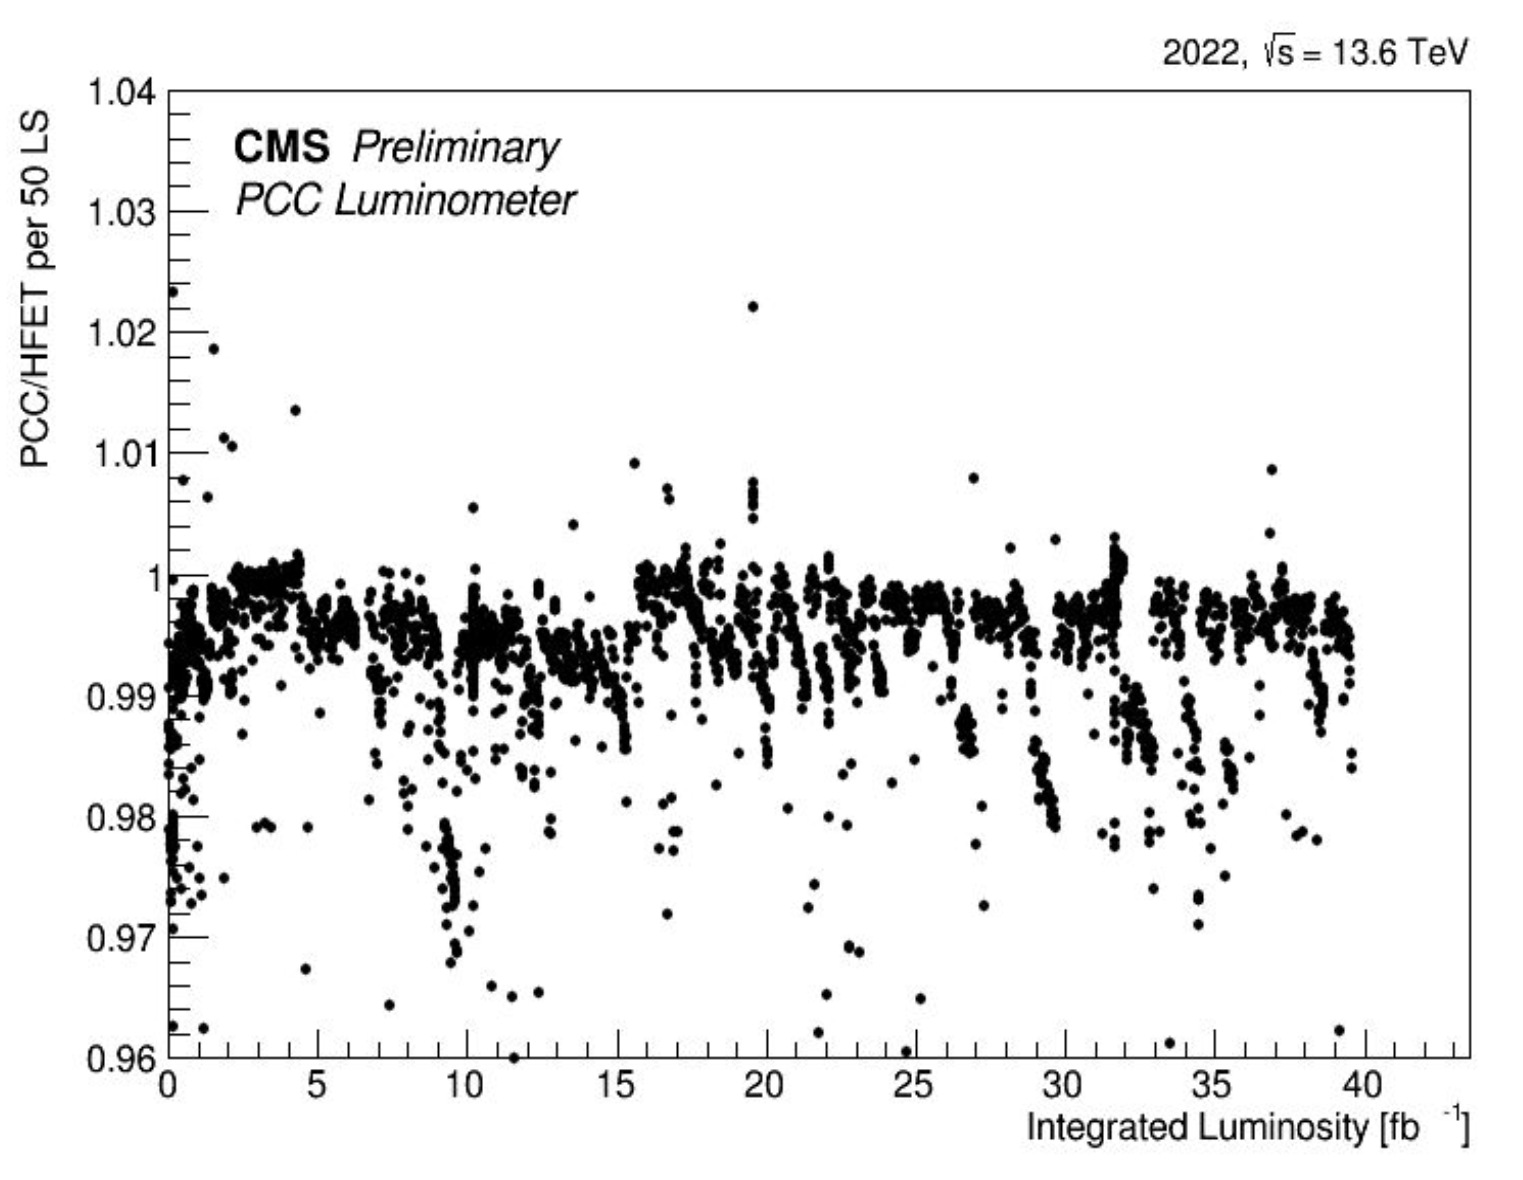
\includegraphics[width=\textwidth]{ashish_thesis/PCC_HFOCvsls_ProfileX_all_2022_1.png}
    %\caption{Image 1}                                                                                                                                                                                 
  \end{subfigure}
  \hfill % or \hspace{5mm} for a specific horizontal space                                                                                                                                                      
  %\begin{subfigure}[b]{0.49\textwidth}
   % 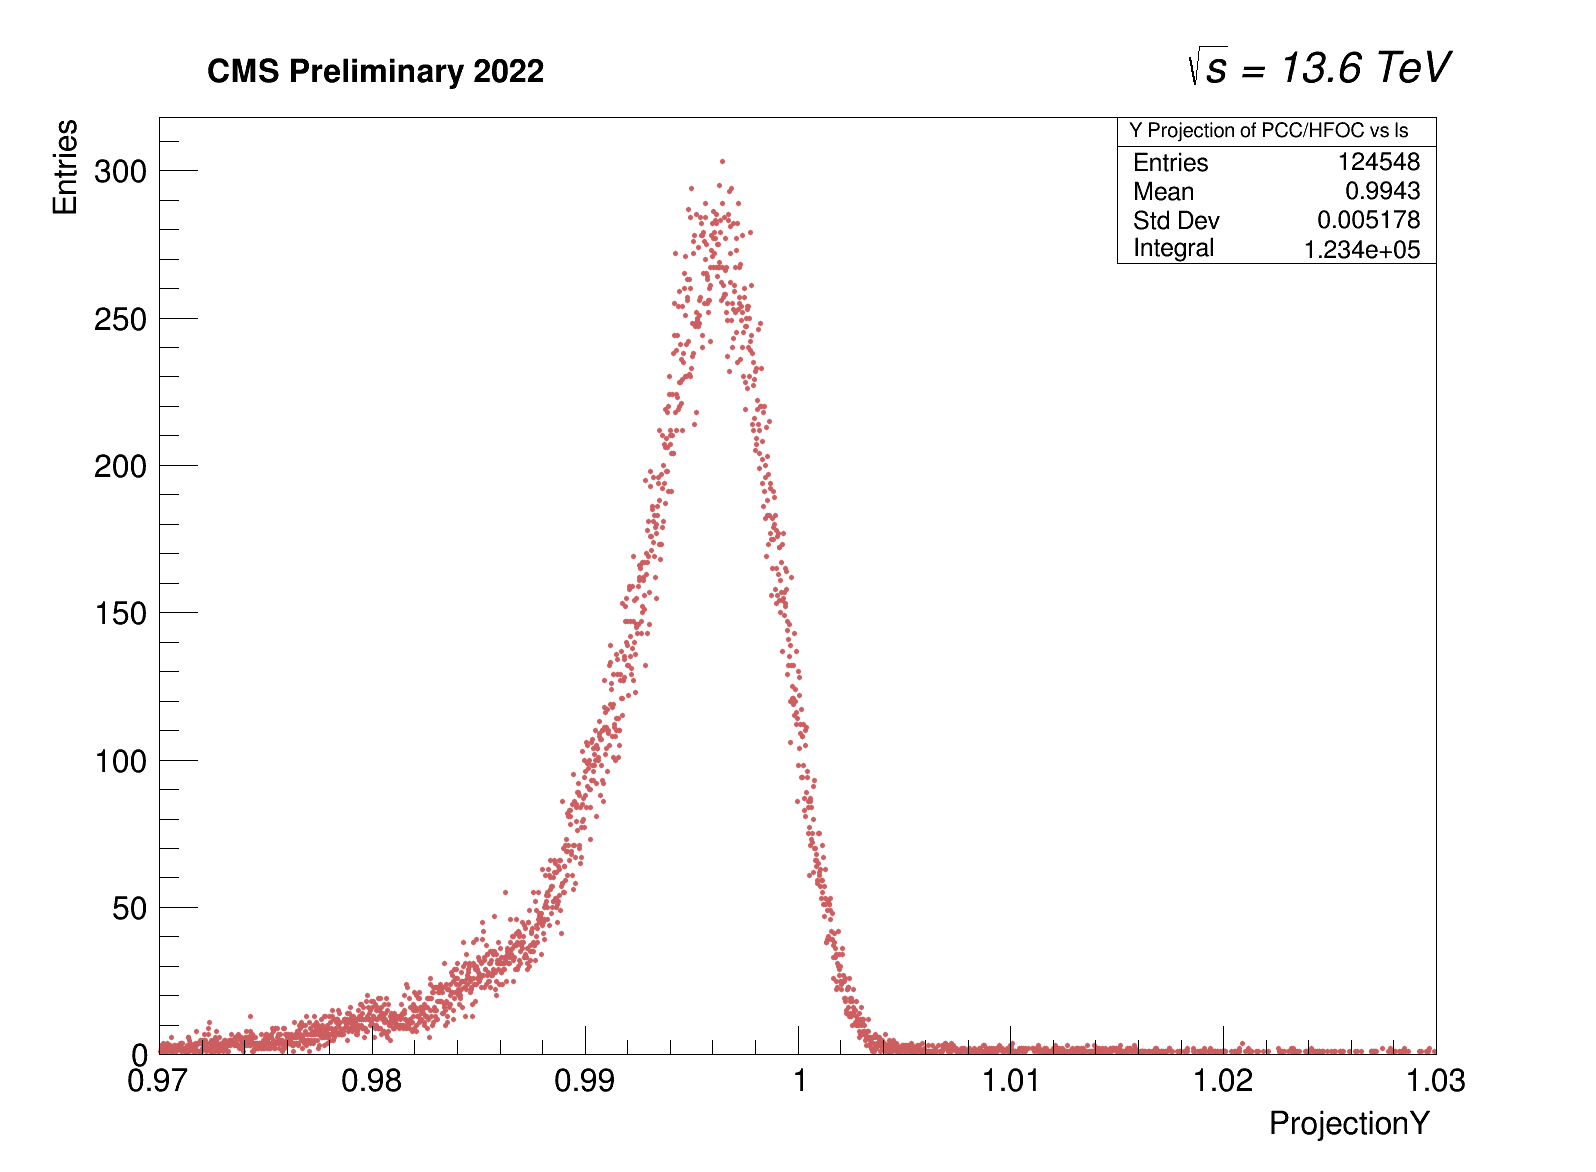
\includegraphics[width=\textwidth]{ashish_thesis/PCCvsHFOC_ProjectionY_all_2022.png}
    %\caption{Image 2}                                                                                                                                                             
  %\end{subfigure}
  \caption[Luminosity ratio profile]{Profile of the PCC/HFET luminosity as a function of integrated luminosity.} %Right: Histogram filled with the ratio of PCC/HFET luminosity per lumi section.}
\label{fig:stabprof_78}
\end{figure}


\begin{figure}[!htp]
\centering
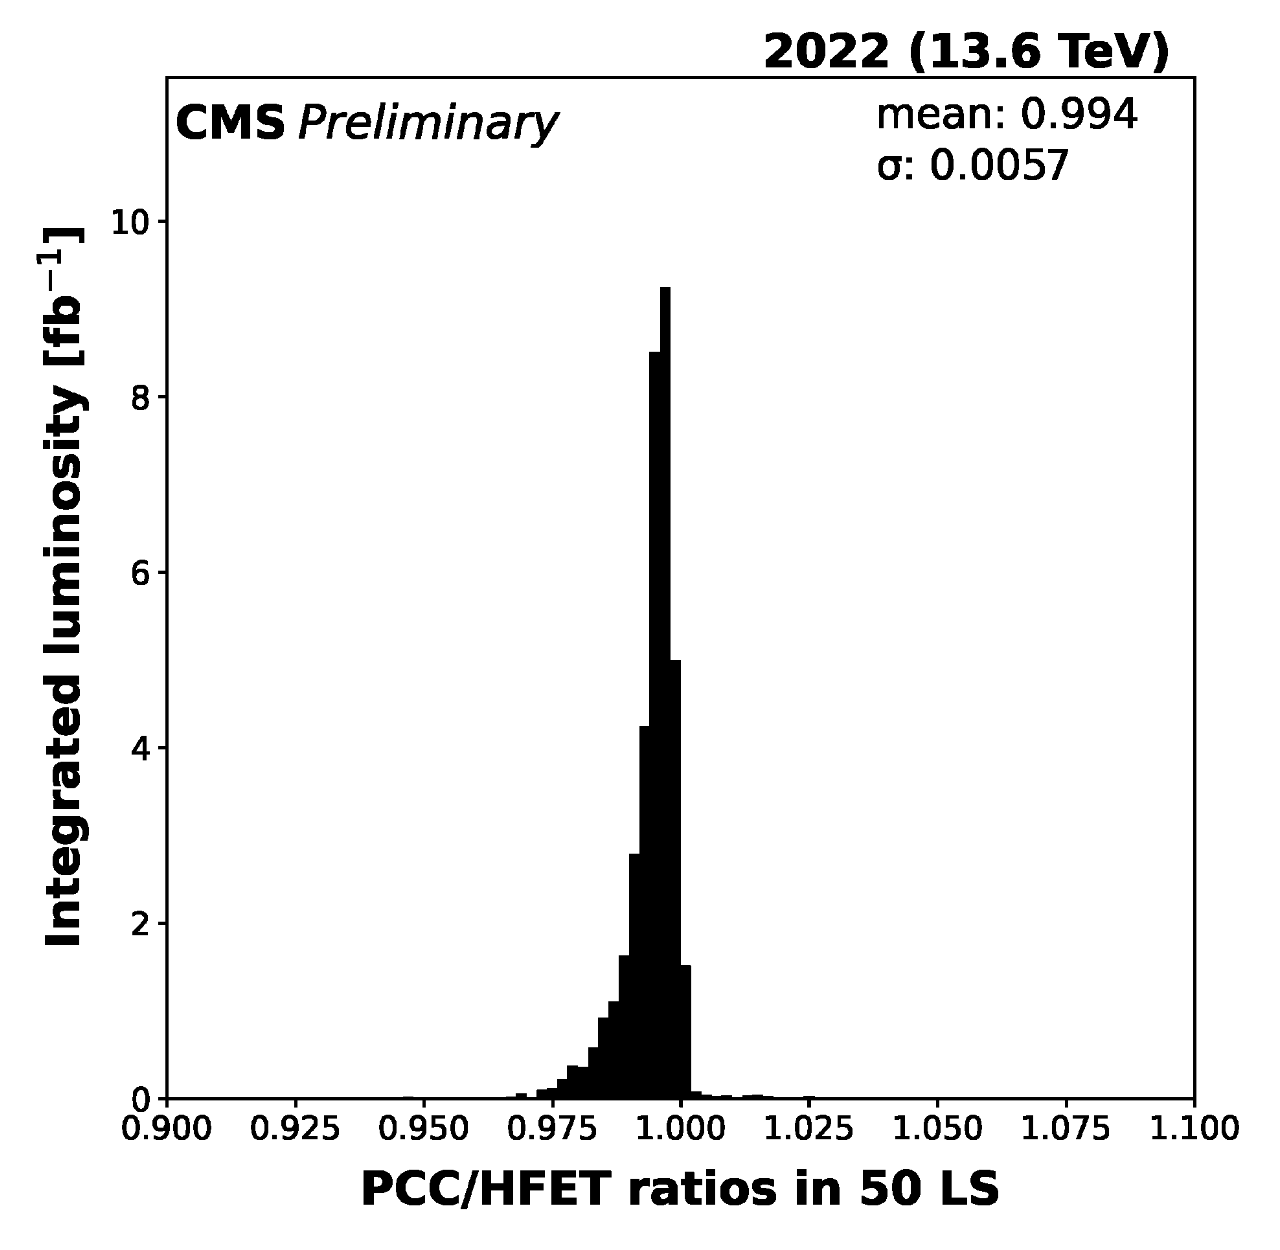
\includegraphics[width=1\textwidth]{ashish_thesis/ProjY_ProfileX_h_ratio_all_2022_1_new.png}
\caption[Projection of luminosity ratio profile]{%                                                                                                                                                                                           
 Distribution of the ratio of PCC/HFET luminosity evaluated per 50 lumi section blocks.
}
\label{fig:stabprof1_79}
\end{figure}

\newpage
\item Linearity: Detectors in high-energy physics experiments can display varying responses at different luminosity levels, leading to non-linear behavior, especially at high luminosities. %This variability is observable in the residuals of PCC luminosity compared to HFOC luminosity.
To quantify the linearity systematic uncertainty, the slope variability of the detector response against luminosity levels can be analyzed. This, combined with the luminosity range, provides a measure of the expected rate variability due to non-linearity, representing the linearity systematic uncertainty \cite{pas_22}. %Non-linear response during fill 8274 and three consecutive fill 8274, 8275 and 8276 is shown in Fig. \ref{fig:kinknon1_} and \ref{fig:kinknon_}.

%"Kink" non-linearity is a specific type of response variation that we observed during 2022 fill  \cite{calibratedRunIIIPCC_AN-22-148}. This phenomenon is characterized by a sudden drop or "kink" in luminosity measurement in the middle of the fill, rather than a gradual or linear change as shown in Fig. \ref{fig:kinknon1_}. This behavior represents a distinct form of non-linearity where the detector's response to particle flow isn't consistent throughout the fill. Instead of maintaining a steady response, the detector experiences an abrupt change, causing a sudden decrease in the measured luminosity. This behaviour is not confined to a particular Fill but can be seen in three consecutive Fill in Fig. \ref{fig:kinknon_}. The root causes of this type of non-linearity is still unknown, potentially could be linked to changes in detector conditions, particle flux inconsistencies, or other experimental variables. A different approach to vetoing modules was able to fix this issue. %Efforts are ongoing to  understand and correct for kink non-linearity to achieve accurate luminosity measurement and reduce systematic uncertainty.

%\begin{figure}[!htp]
%\centering
%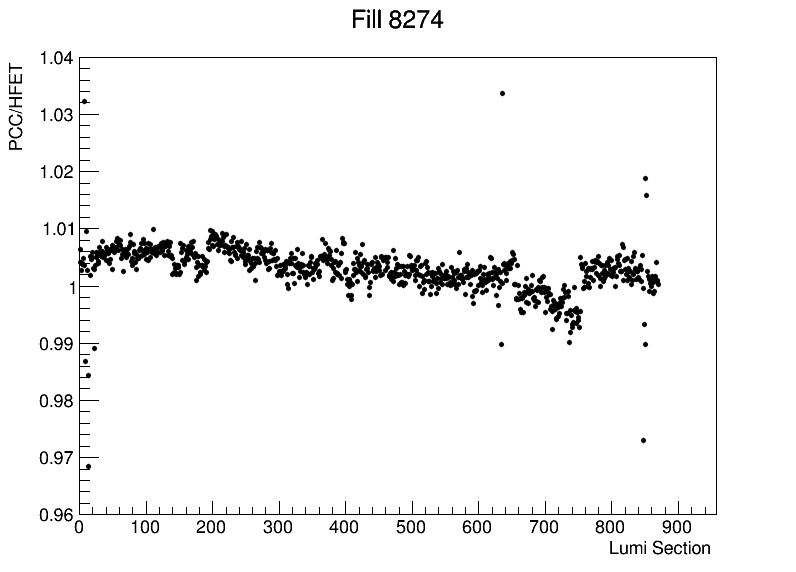
\includegraphics[width=0.6\textwidth]{ashish_thesis/Kink_nonlinearity_oneFill.png}
%\caption[]{%                                                                                                                                                                                                                                             
%Non-linearity during Fill 8274.
%}
%\label{fig:kinknon1_}
%\end{figure}
  
%\begin{figure}[!htp]
%\centering
%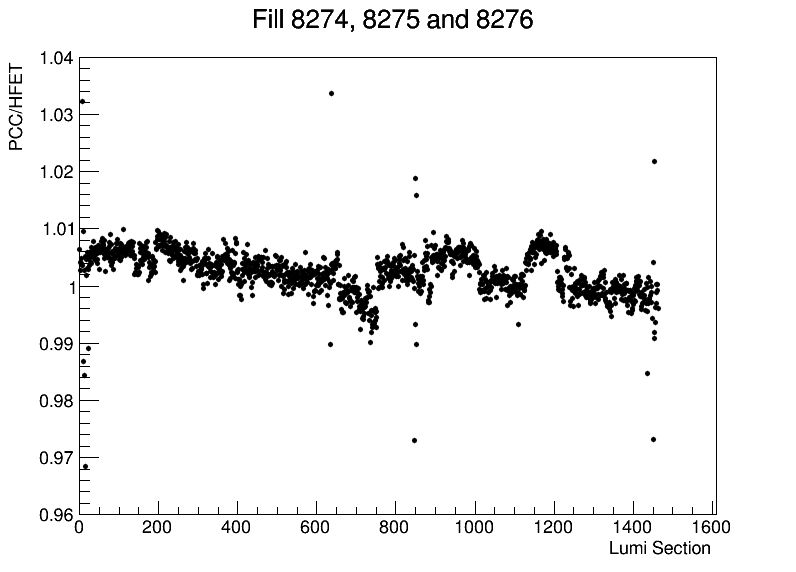
\includegraphics[width=0.6\textwidth]{ashish_thesis/2022_PCC_hfet_nonlinearity.png}
%\caption[]{%                                                                                                                                                                                                                        
%Non-linearity during 3 consecutive Fill 8274, 8275, 8276.
%}
%\label{fig:kinknon_}
%\end{figure}

%The plot in figure \ref{fig:stabprof2_2000} provides a comparison of the linearity of PCC luminosity in relation to HFET luminosity. A perfectly linear relationship would imply same luminosity measured by both the luminometers, suggesting an absence of non-linearity in the detector response.
The plot in Fig. \ref{fig:stabprof2_2000} shows the ratio of luminosity values obtained using the PCC method to those from the HFET luminometer. The values are plotted as a function of HFET luminosity. The goal of this graph is to examine potential changes in the detector response across different luminosity levels. If the detector response was perfectly linear, we do expect the ratio to remain constant across the range of HFET luminosity values. Deviations from a constant ratio indicate non-linearity in the detector response, thereby contributing to systematic uncertainties.

%Linearity of PCC Compared to HFET and Residuals Obtained After Doing a Linear Fit: The left plot in figure \ref{fig:stabprof2_99} provides a visual comparison of the linearity of PCC luminosity in relation to HFET luminosity. A perfectly linear relationship would imply a constant ratio across all luminosity levels, suggesting an absence of non-linearity in the detector response. On the right, the residuals, i.e., the differences between the observed values (PCC/HFET ratio) and the values predicted by a linear fit, are plotted. If the residuals are randomly scattered around zero across all HFET luminosity values, this would support the assumption of linearity. However, if there's a systematic pattern in the residuals, it would suggest non-linearity, indicating potential sources of systematic uncertainty.

\begin{comment}

\begin{figure}[!htp]
\centering
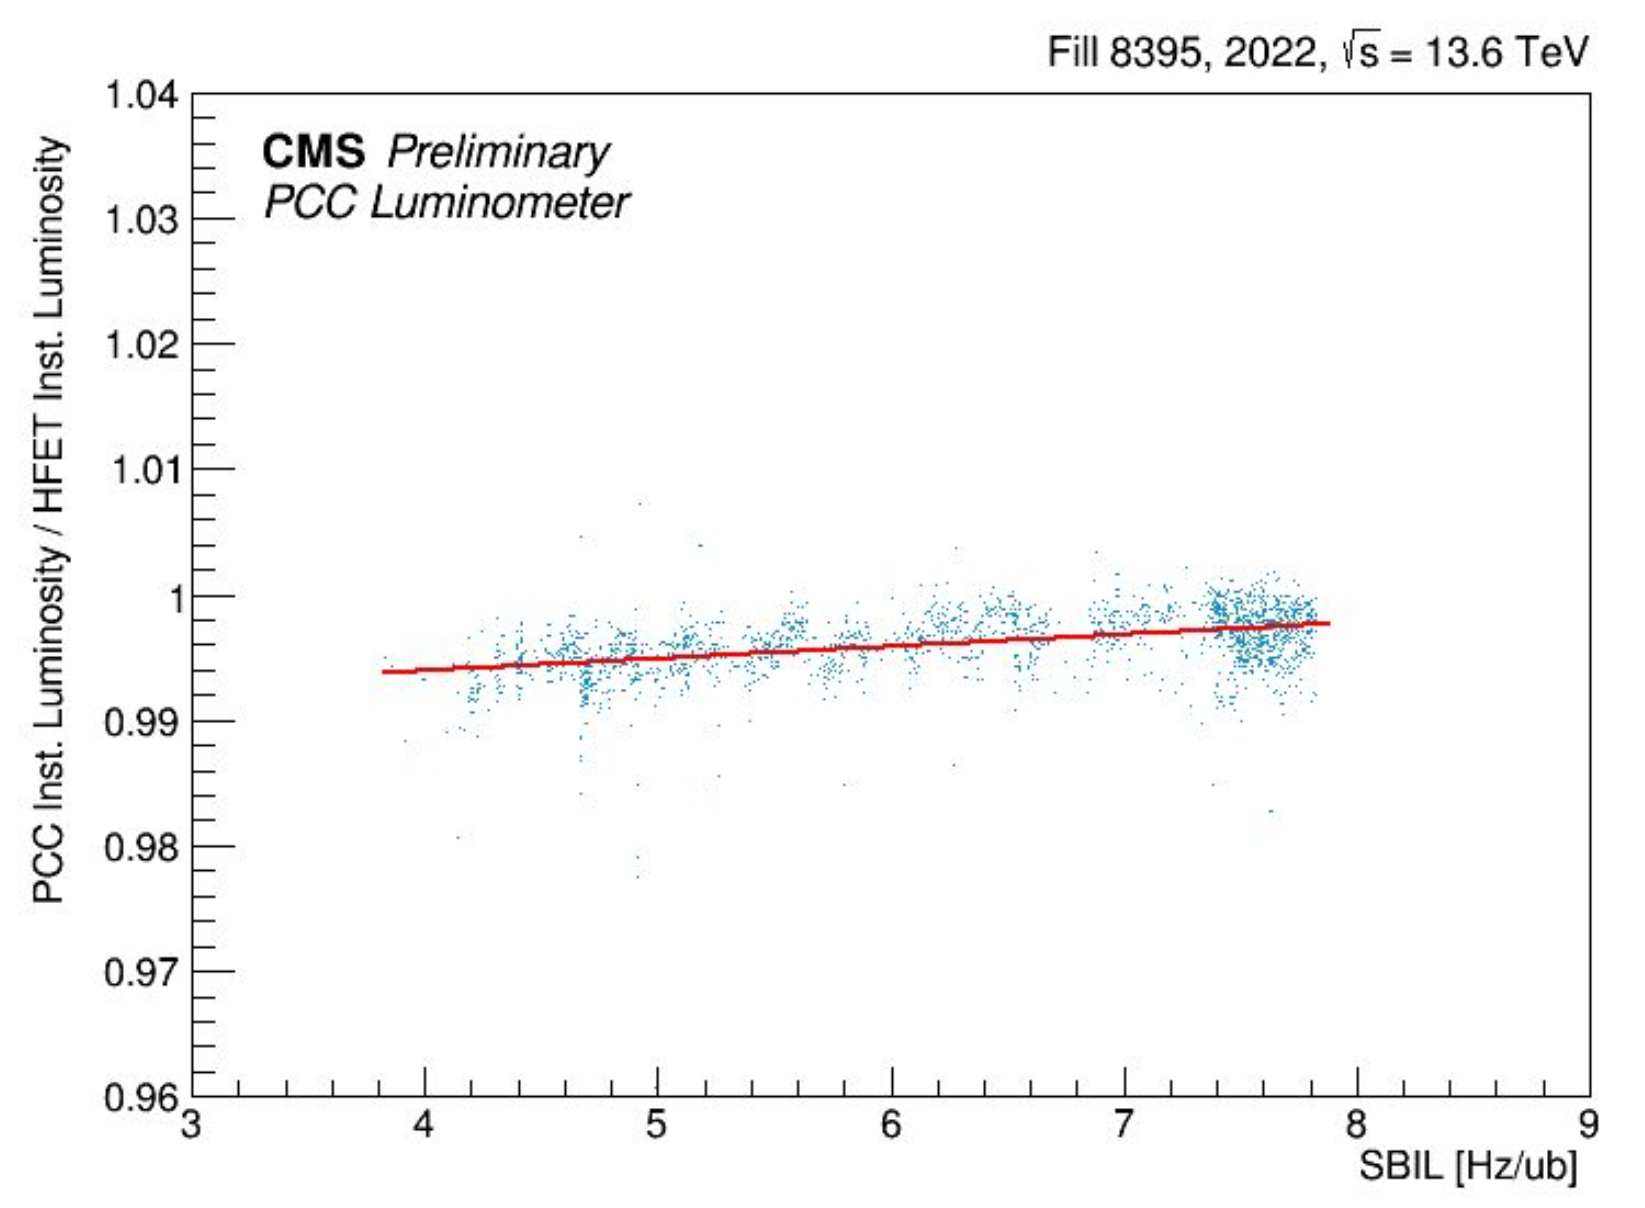
\includegraphics[width=0.6\textwidth]{ashish_thesis/PCC_HFOCvsHFOC_ProfileX_all_2022_1.png}
\caption[PCC response to luminosity]{%                                                                                                                                                                
   Ratio of PCC/HFET luminosity plotted as a function of HFET luminosity to determine change in detector response over different luminosity levels.                                                    
}
\label{fig:lin_unc}
\end{figure}

\end{comment}

%\begin{table}[h]
 % \centering
 % \caption{Parameter values from fit}
  %  \begin{tabular}{ccccc}
   %      Parameter Name & Value & Error \\
    %    \hline
     %    Slope & 2.76132e-07 & 2.97602e-09 \\
      %   Intercept & 9.90718e-01 & 4.73417e-05 \\
    %\end{tabular}
    %\caption{Parameter values from fit}
    %\label{tab:lin_fit_47}
%\end{table}
                                                                                                                                                                                               
\begin{figure}[H]
  \centering
  %\begin{subfigure}[b]{0.49\textwidth}
   % 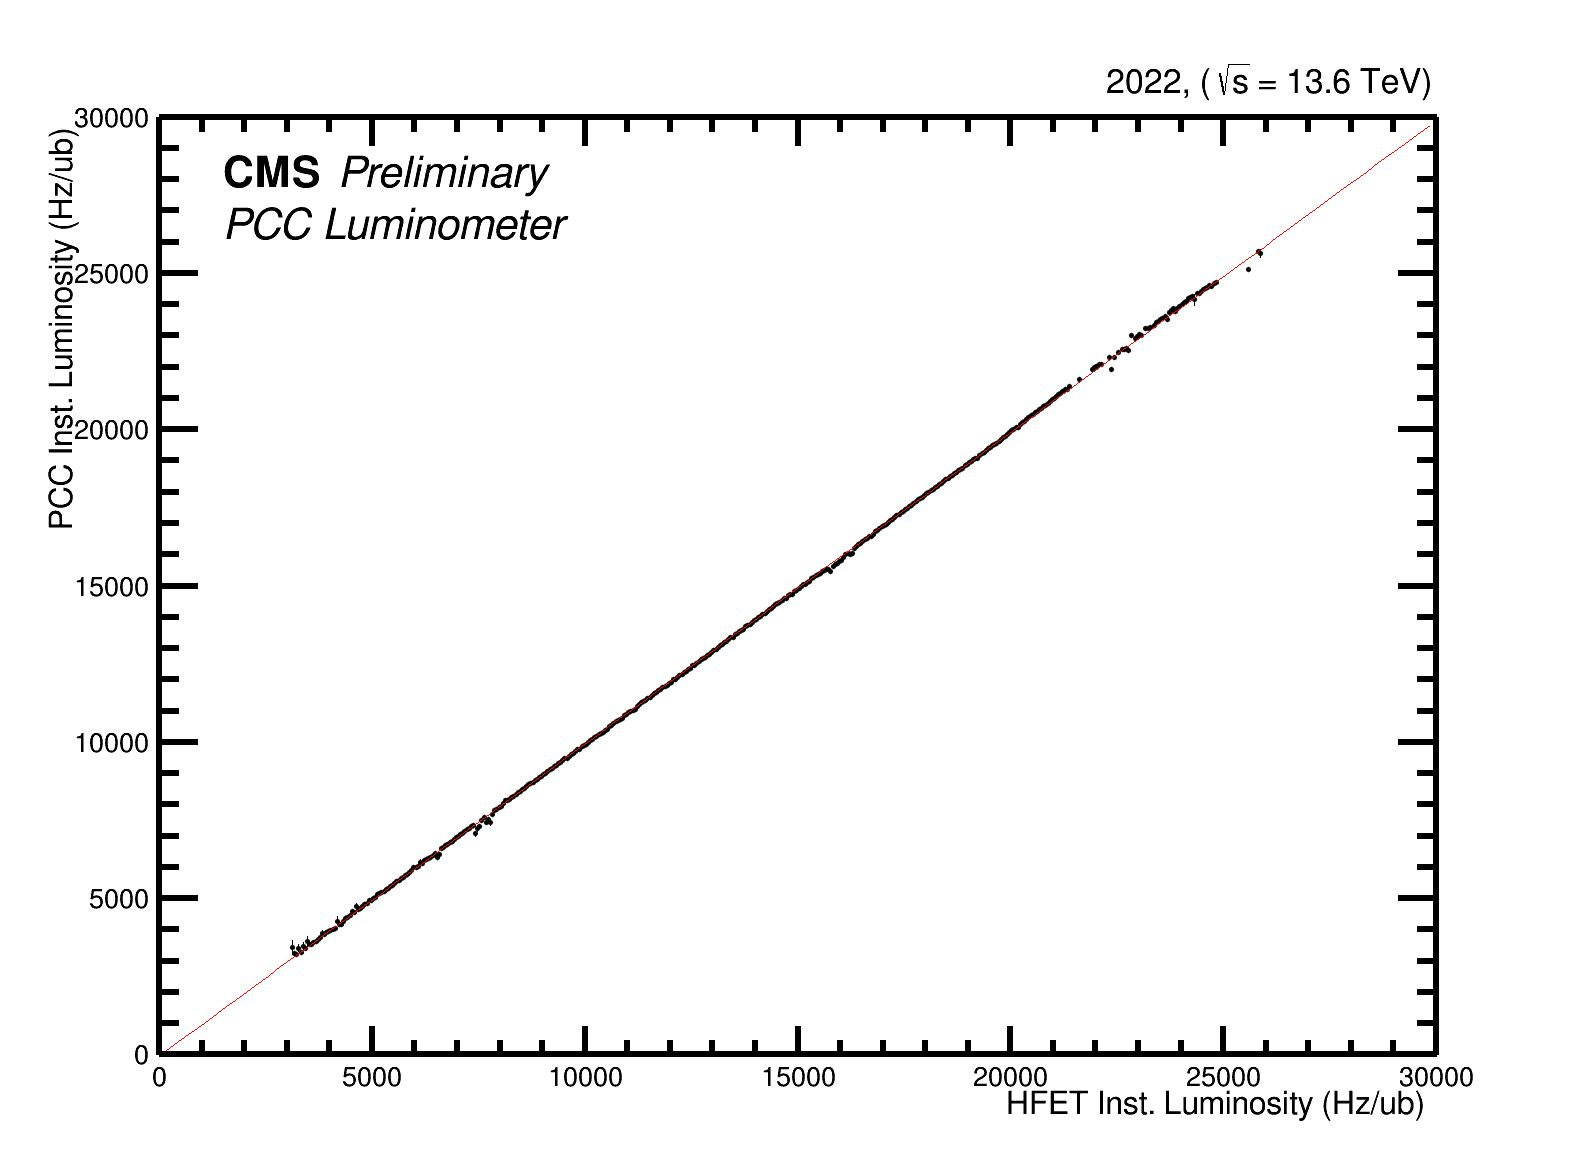
\includegraphics[width=\textwidth]{ashish_thesis/PCCvsHFOC_ProfileX_all_2022.png}
    %\caption{Image 1}                                                                                                                                                                           
  %\end{subfigure}
  %\hfill % or \hspace{5mm} for a specific horizontal space                                                                                                                            
  %\begin{subfigure}[b]{0.49\textwidth}
    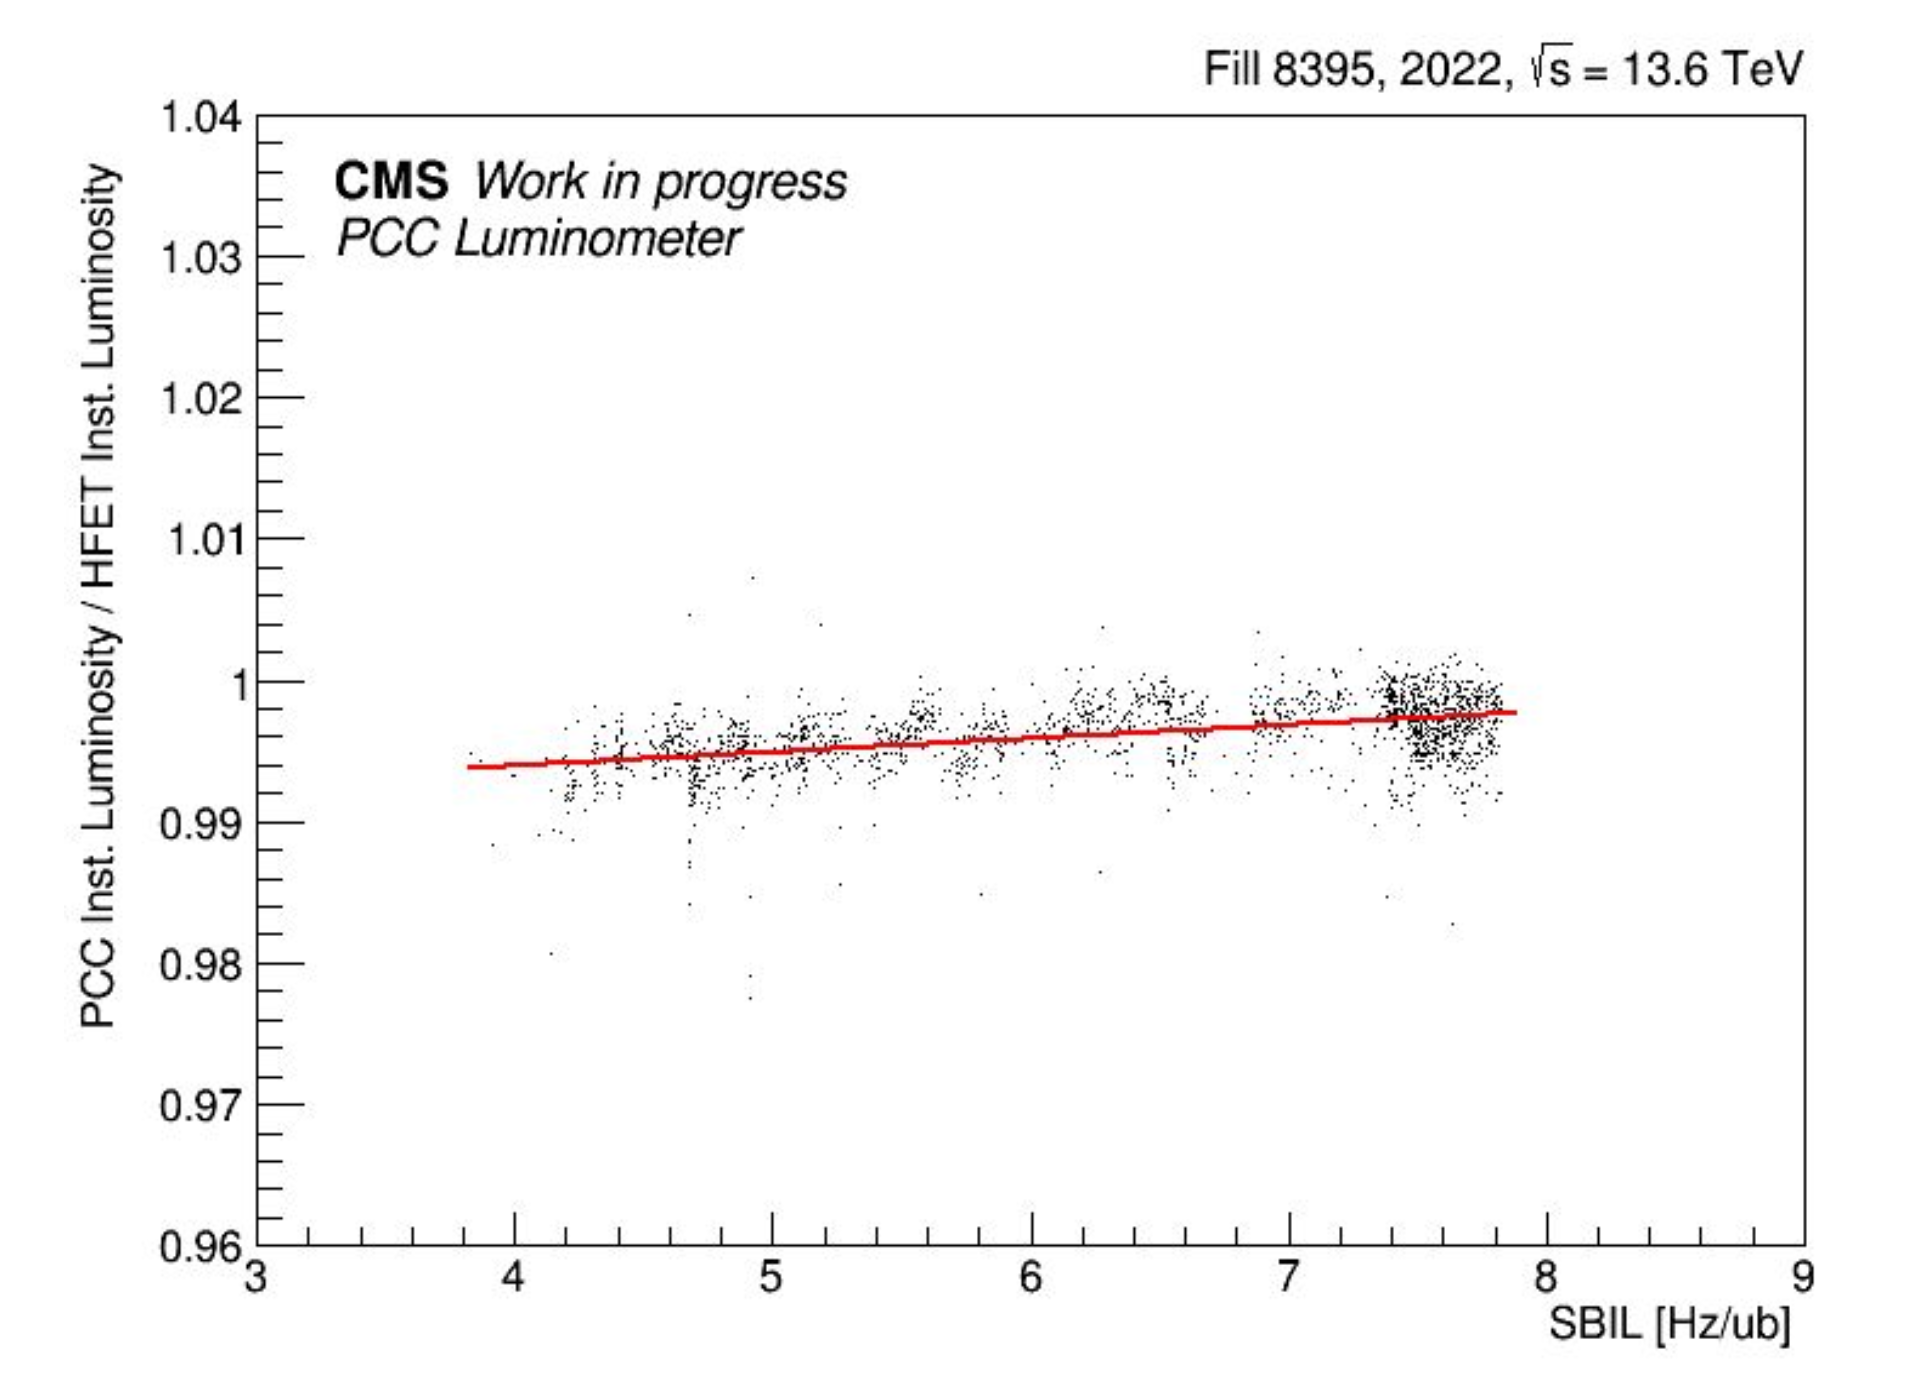
\includegraphics[width=0.7\textwidth]{ashish_thesis/PCC_HFOCvsHFOC_ProfileX_all_2022_1_new.png}
    %\caption{Image 2}                                                                                                                                                                           
  %\end{subfigure}
    \caption[2022 PCC linearity]{%Left: Linearity of PCC compared to HFET.
      Ratio of PCC/HFET luminosity plotted as a function of HFET luminosity to determine change in detector response over different luminosity levels. Slope is 0.00114 ub/Hz. % $ PCC and HFET iovtags used are pcc22v2 and hfet22v10.$
  }

\label{fig:stabprof2_2000}
\end{figure}

\item Afterglow: Systematic uncertainties from afterglow backgrounds are derived from the means of type 1 and type 2 afterglow residuals. These are determined by comparing the luminosity of the immediate empty bunch after a collision to the colliding bunch luminosity and comparing subsequent empty bunches' luminosity to the colliding bunch, respectively.

%\begin{figure}[!htp]
%\centering
%\includegraphics[width=1\textwidth]{ashish_thesis/afterglow_t1f_vsinstlumi.png}
%\caption[2022 PCC type 1 afterglow fraction]{%
 % PCC afterglow correction type 1 fraction as a function of instantaneous luminosity for period Run 2022F. The residual fraction is given by the ratio of the luminosity of the first empty bunch immediately following a colliding bunch to the luminosity of the colliding bunch.

%}
%\label{fig:period_bound_44}
%\end{figure}

%\begin{figure}[H]
%\centering
%\includegraphics[width=1\textwidth]{ashish_thesis/afterglow_t1res_vsinstlumi_1.png}
%\caption[2022 PCC Type 1 Afterglow Residuals]{%                                                                                                                                                                             
 %PCC afterglow correction type 1 residual as a function of instantaneous luminosity for period Run 2022F. The residual fraction is given by the ratio of the luminosity of the first empty bunch immediately following a colliding bunch to the luminosity of the colliding bunch.

%}
%\label{fig:period_bound_44}
%\end{figure}

%\begin{figure}[H]
%\centering
%\includegraphics[width=1\textwidth]{ashish_thesis/afterglow_t2res_vsinstlumi_1.png}
%\caption[2022 PCC Type 2 Afterglow Residuals]{%
 % Type 2 residual as a function of instantaneous luminosity for period 2022F. These are given by the ratio of the luminosity of the second and following empty bunches after a colliding bunch to the luminosity of the colliding bunch.
%}
%\label{fig:period_bound_45}
%\end{figure}

\end{itemize}

Table \ref{table:correction_uncertainties} provides a detailed breakdown of the systematic uncertainties associated with the luminosity measurement for the year 2022. Each row represents a specific correction factor, while the corresponding column indicates its associated uncertainty as a percentage. 

\begin{table}[H]
  \centering
  \caption[Systematic uncertainty in 2022 luminosity measurement]{Systematic uncertainty in 2022 PCC luminosity measurement (\%) \cite{pas_22}}
    \begin{tabular}{l|c}
        \textbf{Source} & \textbf{Uncertainty (\%)} \\
        \hline
        \multicolumn{2}{c}{\textbf{Calibration}} \\
        \hline
        Beam current & 0.2 \\
        Ghost and satellite charges & 0.2 \\
        Orbit drift & 0.1 \\
        Residual beam positions & 0.3 \\
        Beam-beam effects & 0.4 \\
        Length scale & 0.1 \\
        Factorization bias & 0.8 \\
        Scan-to-scan variation & 0.5 \\
        Bunch-to-bunch variation & 0.1 \\
        Cross-detector consistency & 0.4 \\
        \hline
        \multicolumn{2}{c}{\textbf{Integration}} \\
        \hline
        Afterglow corrections & 0.2 \\
        Cross-detector stability & 0.6 \\
        Cross-detector linearity & 0.5 \\
        \hline
        Calibration & 1.2 \\
        Integration & 0.8 \\
        \hline
        \textbf{Total} & 1.4 \\
    \end{tabular}
    \label{table:correction_uncertainties}
    %\caption{Systematic uncertainty in luminosity measurement (\%)}
\end{table}


\begin{comment}

\section{Uncertainties associated with the Van der Meer calibration}

\begin{itemize}
    
\item Orbit Drift: Refers to the gradual displacement of the beam orbit from its ideal trajectory due to various effects such as ground motion, magnetic field fluctuations, and thermal expansion. This can result in reduced beam intensity and beam quality.

\item X-Y Nonfactorization: Refers to the failure of the x and y coordinates of a particle beam to factorize, meaning that the beam profile cannot be expressed as a product of independent x and y profiles. This can result in beam asymmetries and other effects.

\item Beam-Beam Deflection: Refers to the mutual interaction of two colliding particle beams, resulting in the deflection of the individual beams due to the electromagnetic fields generated by the other beam. This effect can lead to beam losses and reduced luminosity.

\item Dynamic $\beta$: Refers to the time-varying beta function of a particle beam, which describes the rate at which the beam diverges or converges as it propagates. This effect can be important for beam stability and the control of beam emittance.

\item Beam Current Calibration: Refers to the process of accurately measuring the current of a particle beam, which is essential for many beam diagnostics and control systems.

\item Ghosts and Satellites: Refers to unwanted signals in a detector or measurement system that can arise from various sources such as scattered radiation, electronic noise, or interference from other particles. These can lead to inaccurate measurements and reduced data quality.

\item Scan to Scan Variation: Refers to the variation in experimental results obtained from different scans or measurements, which can arise from various sources such as statistical fluctuations, instrument drift, or systematic errors.

\item Bunch to Bunch Variation: Refers to the variation in the properties of individual particle bunches within a beam, such as their intensity, energy spread, or emittance. This effect can be important for beam tuning and optimization.

\item Cross-Detector Consistency: Refers to the agreement between measurements obtained from different detectors or measurement systems. This is important for verifying the accuracy and reliability of experimental results.

\item Background Subtraction: Refers to the process of removing unwanted signals from a measurement or detector system that arise from sources other than the physical phenomenon of interest, such as noise, cosmic rays, or other particles. This is essential for obtaining accurate measurements of the physical signal.

\end{itemize}

\section{Uncertainties associated with physics data taking}

\begin{itemize}

\item Stability: The CMS pixel detector is a complex instrument with many components, including silicon sensors and readout electronics, that must operate consistently and with high precision over long periods. Any variations in the performance of the detector can affect the efficiency of the pixel cluster counting method and lead to uncertainties in the luminosity measurement.

One example of how the stability of the detector can affect the luminosity measurement is through changes in the detector's noise level. The noise level refers to the level of electronic noise present in the detector, which can interfere with the detection of pixel clusters produced by proton-proton collisions. If the noise level increases, the efficiency of the pixel cluster counting method may decrease, leading to an underestimation of the luminosity. Conversely, if the noise level decreases, the efficiency of the method may increase, leading to an overestimation of the luminosity.

Another example is changes in the efficiency of the pixel detector. The efficiency of the detector refers to the fraction of proton-proton collisions that produce pixel clusters that can be detected and counted by the method. Any changes in the efficiency of the detector, for example due to changes in the gain or response of the silicon sensors, can lead to uncertainties in the luminosity measurement.

To mitigate these uncertainties, the CMS collaboration performs regular calibrations and monitoring of the detector performance, as well as cross-checks with other luminosity measurement techniques

Systematic uncertainties due to stability in the detector itself for the pixel cluster counting method are typically estimated by studying the performance of the method over time and comparing it to simulations or other measurements. Uncertainties due to changes in the noise level and detector efficiency are typically estimated separately and combined to obtain the total systematic uncertainty

\item Linearity: the luminosity obtained from the PCC method is compared to that obtained from the HFOC method for a given set of collisions. Any deviations between the two measurements are used to estimate the linearity uncertainty in the PCC method.

The linearity uncertainty is typically quantified as a systematic uncertainty in the luminosity measurement, expressed as a percentage of the measured luminosity. This uncertainty can be estimated by fitting the PCC and HFOC measurements to a linear function and calculating the deviation of the PCC measurement from the linear fit.

\item Type 1 afterglow refers to the persistence of charge in the pixels of the detector after a collision event. This charge can be produced by various sources, such as ionization due to the passage of charged particles, or leakage currents in the readout electronics. If this charge is not properly accounted for, it can be mistakenly counted as pixel clusters produced by subsequent collision events, leading to an overestimation of the luminosity.

Type 2 afterglow refers to the persistence of noise in the detector after a collision event. This noise can be produced by various sources, such as thermal or radiation-induced effects, and can also interfere with subsequent collisions. If this noise is not properly accounted for, it can lead to a reduction in the efficiency of the pixel cluster counting method and an underestimation of the luminosity.

\end{itemize}



\section{Comparison of PCC with HFOC luminosity}

\end{comment}
